	%%%%%%%%%%%%%%%%%%%%%%%%%%%%%%%%%%%%%%%%%%%%%%%%%%%%%%%%%%%%%%%%%%%%%%%%%%%%%%%%%%%%%%%%%%%%%%%%%%%%%
%
%   Version     : 2.0
%
%   Filename    : main.tex
%
%   Description : This is the main file for the LaTeX thesis proposal document template.
%                 The template is intended for use by BSCS students. 
%
%                It is assumed that you can learn how to use LaTeX on your own.
%                Please check/read the following online LaTeX book:
%
%                                 http://en.wikibooks.org/wiki/LaTeX
%     
%   Author      : Florante R. Salvador
%
%   Contributors: 1.  Kebin Batak Chan
%				  2.  Kevin Chan
%                     a. margin settings for DLSU thesis paper 
%   
%ee
%  Reference:
%
%
%   History/Updates:
%      March 12, 2009 -- created version 1.0 for release to CSC701M (Methods of Research) students
%      May 30, 2009   -- updated Title page and Abstract for undergrad ST students
%
%      Feb 27, 2015 -- Created Version 2 (major overhaul): changed class to report, created a figures folder, 
%                               removed unnecessary packages, added new comments  based on Ethel Ongs slides
% pogi si migo we're back boyx
%%%%%%%%%%%%%%%%%%%%%%%%%%%%%%%%%%%%%%%%%%%%%%%%%%%%%%%%%%%%%%%%%%%%%%%%%%%%%%%%%%%%%%%%%%%%%%%%%%%%%%

%!TEX root = main.tex
%%%%%%%%%%%%%%%%%%%%%%%%%%%%%%%%%%%%%%%%%%%%%%%%%%%%%%%%%%%%%%%%%%%%%%%%%%%%%%%%%%%%%%%%%%%%%%%%%%%%%%%%%%%%%%%%%%%%%%%
%
%  Filename   : preamble.tex
%
%  Description: Preamble file to :
%               a. specify related packages
%               b. set margins, commands, etc.
%
%  Note       : Edit the margin settings for your own printer
%                  You may add your own commands, environments (it is assumed that you know what you're doing.)
%
%%%%%%%%%%%%%%%%%%%%%%%%%%%%%%%%%%%%%%%%%%%%%%%%%%%%%%%%%%%%%%%%%%%%%%%%%%%%%%%%%%%%%%%%%%%%%%%%%%%%%%%%%%%%%%%%%%%%%%%

%\documentclass[12pt,titlepage,onepage, letterpaper]{article}

\documentclass[12pt,titlepage,onepage, letter]{report}


%
%-- specify related packages
%

%
% \usepackage[utf8x]{inputenc}
%

\usepackage{apacite}           %-- APA style citation 
                               %-- refer to http://www.ctan.org/tex-archive/biblio/bibtex/contrib/apacite/

%
%  \usepackage{ucs}
%


\usepackage{amsmath}           %-- American Math Society packages
\usepackage{amsfonts}
\usepackage{amssymb}
\usepackage{titlesec}

\usepackage{graphicx}          %-- graphicx package needed for including figures in JPG or PNG format
\graphicspath{ {figures/} }

\usepackage{float} 
%
%\usepackage{graphics}          %-- graphics related package (this was commented out) use when image is in EPS format
%

\usepackage{verbatim}          %-- this package allows you to have multiple lines of comments by
                               %-- example:
                               %   \begin{comment}
                               %        ...your text here...
                               %   \end{comment}  

\usepackage{color}             %-- allows use of color with text
                               %-- example:  \textcolor{red}{This is the colored text in red.}

\usepackage{url}  %-- allows use of URLs example: \url{https:\ccs1.dlsu.edu.ph}
\usepackage{makecell} % Used for cell formatting
\usepackage{longtable}
\usepackage{rotating}

\usepackage{booktabs}
\usepackage{array,booktabs,ragged2e}
\usepackage{colortbl}
\usepackage[table]{xcolor}
\usepackage{bm}
\usepackage{outlines} 

\newcolumntype{R}[1]{>{\RaggedLeft\arraybackslash}p{#1}}

%
%-- set margins,  you may need to edit this for your own printer
%
\topmargin 0.65in
\oddsidemargin 0.5in
\evensidemargin 0.5in

\voffset 0.0in
\hoffset 0.0in

\textwidth 5.75in
\textheight 7.0in


\parskip 1em
\parindent 0.25in

\bibliographystyle{apacite}            %-- use APA citation scheme

\hyphenation{ana-lysis know-ledge}     %-- LaTeX may not hyphenate correctly some words you use in your document
                                       %-- use \hyphenation to instruct LaTeX how to do it correctly, example above

\newcommand{\degree}{^{\circ}}         %-- use \newcommand to create your own "commands"
                                       %-- \newcommand works like the #define you learned in your COMPRO1 class

\newcommand{\etal}{et al.}


%\newcommand{\sinag}{\emph{Sinag}}
%\newcommand{\sinagtwo}{\emph{Sinag2}}

\newcommand{\figref}[1]{Figure \ref{#1}}
\newcommand{\appref}[1]{Appendix \ref{#1}}

%-- \newcommand{\Section}[1]{\section{#1}\setcounter{figure}{0}\setcounter{table}{0}}

%\newcommand{\shade}{\multicolumn{1}{|>{\columncolor[gray]{0.25}}c|}{}}
%\newcommand{\tableheader}[1]{\rowcolor{black}\color{white}{#1}}
%\newcommand{\cell}[2]{\multicolumn{1}{#1}{#2}}
%\newcommand{\definition}[2]{\textbf{\textit{#1}} --- #2}
%\newcommand{\itembit}[1]{\item \textbf{\textit{#1}}}
%\newcommand{\sgdef}[2]{\parbox[t][][t]{1.75in}{\textbf{#1}} \> \parbox[t][][t]{4.0in}{#2}\\\\}

%\newenvironment{sinagglossary}{\begin{flushleft}
%\begin{tabbing}
%\hspace{1.75in}\=\\}{\end{tabbing}\end{flushleft}}

\newcommand{\thestitle}[1]{{\Large \textsc{#1}}}

\usepackage{titlesec}

\setcounter{secnumdepth}{5}
\setcounter{tocdepth}{2}

\titleformat{\paragraph}
{\normalfont\normalsize\bfseries}{\theparagraph}{1em}{}
\titlespacing*{\paragraph}
{0pt}{3.25ex plus 1ex minus .2ex}{1.5ex plus .2ex}

\titleformat{\subparagraph}
{\normalfont\normalsize\bfseries}{\theparagraph}{1em}{}
\titlespacing*{\subparagraph}
{0pt}{3.25ex plus 1ex minus .2ex}{1.5ex plus .2ex}




%---
%  \renewcommand{\thefigure}{\thesection.\arabic{figure}}
%  \renewcommand{\thetable}{\thesection.\arabic{table}}
%  \renewcommand{\contentsname}{Table of Contents}




                %-- includes LaTeX source file for the preamble 
                                  %-- include packages, sets the margin sequence, and many more... 
\usepackage{csquotes}
\usepackage{enumitem}
\usepackage{epigraph}
\usepackage{sidecap}
\usepackage{wrapfig}
\usepackage{graphicx}
\usepackage{ltxtable}
\usepackage{rotating} % you need this for the sidewaystable
\usepackage{caption} % you need this for the caption
\usepackage{pdflscape} % you need this for the landscape page 
\usepackage[round]{natbib} % - added to accommodate citet
                                  %-- your job: check if the settings are suitable for your own printer

\graphicspath{{figures/}}  %-- figures is the name of the folder containing images JPG or PN

\begin{document}

%%%%%%%%%%%%%%%%%%%%%%%%%%%%%%%%%%%%%%%%%%%%%%%%%%%%%%%%%%%%%%%%%%%%%%%%%%%%%%%%%%%%%%%%%%%%%%%%%%%%%%
%
%   Filename    : title_page.tex 
%
%   Description : This file will contain your Title Page.
%                 
%%%%%%%%%%%%%%%%%%%%%%%%%%%%%%%%%%%%%%%%%%%%%%%%%%%%%%%%%%%%%%%%%%%%%%%%%%%%%%%%%%%%%%%%%%%%%%%%%%%%%%

\begin{titlepage}
\centering


%-- **EDIT** the following line to indicate your thesis title
\thestitle{Flow: Musical Composition via Gesture Interactions with Musical Metacreation}

\vspace{1.75cm}
A Thesis Proposal\\
Presented to\\
the Faculty of the College of Computer Studies\\
De La Salle University Manila

\vspace{1.75cm}
In Partial Fulfillment\\
of the Requirements for the Degree of\\
Bachelor of  Science in Computer Science

\vspace{1.75cm}
by\\
%-- **EDIT** the following line to indicate your name 
\vspace{1cm}

CHAN, Kevin Gray \\
DANCEL, Migo Andres  \\
GONZALES, Allen Vincent  \\
TOBIAS, John Patrick  \\

\vspace{1.75cm}
%-- **EDIT** the following line to indicate your adviser's name 
Jordan Aiko DEJA \\
Adviser

\vspace{1.75cm}
\today
\end{titlepage}
              
%!TEX root = main.tex
%%%%%%%%%%%%%%%%%%%%%%%%%%%%%%%%%%%%%%%%%%%%%%%%%%%%%%%%%%%%%%%%%%%%%%%%%%%%%%%%%%%%%%%%%%%%%%%%%%%%%%
%
%   Filename    : abstract.tex 
%
%   Description : This file will contain your abstract.
%                 
%%%%%%%%%%%%%%%%%%%%%%%%%%%%%%%%%%%%%%%%%%%%%%%%%%%%%%%%%%%%%%%%%%%%%%%%%%%%%%%%%%%%%%%%%%%%%%%%%%%%%%

\begin{abstract}

\begin{comment}
From 150 to 200 words of short, direct and complete sentences, the abstract 
should be informative enough to serve as a substitute for reading the thesis document 
itself.  It states the rationale and the objectives of the research.  

In the final thesis document (i.e., the document you'll submit for your final thesis defense), the 
abstract should also contain a description of your research results, findings, 
and contribution(s).

%
%  Do not put citations or quotes in the abract.
%

Keywords can be found at \url{http://www.acm.org/about/class/class/2012?pageIndex=0}.  Click the 
link ``HTML'' in the paragraph that starts with ''The \textbf{full CCS classification tree}...''.
\end{comment}

This study explores the design of an interaction that aims to balance the work of composers with the help of a mobile application. Musical composition is a delicate and disciplined art form that is tedious and repetitive. It involves three main activities: ideation, sketching, and revision. Certain compositional tasks such as figuring out succeeding notes often requires trial-and-error. Existing technology has employed musical metacreation to assist in this process. This endows machines with the artificial creative capacity to perform musical tasks. In review, the existing technology has not been generally used in all stages of the musical composition process. By combining several interaction technologies, composers can benefit by being able to do their tasks with significantly less cognitive load and time.

\begin{flushleft}
\begin{tabular}{lp{4.25in}}
\hspace{-0.5em}\textbf{Keywords:}\hspace{0.25em} & Human Centric Computing, Human Computer Interaction, Interaction Design, User Interface Design, Interaction Techniques, Gestural Input, Sound and music computing, Computational creativity, Usability testing \\
\end{tabular}
\end{flushleft}
\end{abstract}
               

\pagenumbering{roman}             %-- this will number pages as i, ii, iii, etc...
\setcounter{page}{2}

\tableofcontents                  %-- this command is testosterone used to generate the Table of Contents


\newpage
\listoffigures                    %-- this command is used to generate List of Figures

\newpage                       
\listoftables                     %-- this command is used to generate List of Tables

\newpage

\pagenumbering{arabic}            %-- this will number pages as 1, 2, 3, etc...
\setcounter{page}{1}              


%!TEX root = main.tex
%%%%%%%%%%%%%%%%%%%%%%%%%%%%%%%%%%%%%%%%%%%%%%%%%%%%%%%%%%%%%%%%%%%%%%%%%%%%%%%%%%%%%%%%%%%%%%%%%%%%%%
%
%   Filename    : chapter_1.tex 
%
%   Description : This file will contain your Research Description.
%                 
%%%%%%%%%%%%%%%%%%%%%%%%%%%%%%%%%%%%%%%%%%%%%%%%%%%%%%%%%%%%%%%%%%%%%%%%%%%%%%%%%%%%%%%%%%%%%%%%%%%%%%

%% ==== Notes from Sir JD: Please answer the questions I'll be putting here



%added by sir jd just for fun
\epigraph{Music is a science which must have determined rules. These rules must be drawn from a principle which should be evident, and this principle cannot be known without the help of mathematics. I must confess that in spite of all the experience which I have acquired in music by practicing it for a fairly long period, it is nevertheless only with the help of mathematics that my ideas became disentangled and that light has succeeded to a certain darkness of which I was not aware before.}{\textit{\citet{rameau1722traite}}}
\chapter{Research Description}
\label{sec:researchdesc}    %--note: labels help you with hyperlink editing (using your IDE)

This chapter is composed of the introduction, overview of the current state of musical metacreation, the research problem, objectives, scope, limitations and significance. The motivation behind the study will also be discussed in this chapter. 

\section{Overview of the Current State of Technology}
\label{sec:overview}
%
%   ==== The Overview of the Current State of Technology should usually contain three main paragraphs that ends with the problem at hand. The last few sentences of this section should be a problematic statement that rougly introduces the reader to the statement of the problem. 
%

%%=== begin with: describing the process of musical composition, then proceed with the what technologies, in summary, have been crafted to assist the musical composition process.

The discipline of composing music can be traced to as far back as ancient Greece \citep{burney1789general}. It is a specific and careful craft that requires many characteristics such as discipline, skill and immense patience. The approach of composing music itself has given birth to newer genres and sub-genres as composers have grown more creative and personal with their creations \citep{miller1984genre}. Some composers even follow a strict set of theories and guidelines to maintain the aesthetic quality of the music they create \citep{rothgeb1975strict,collins2005synthesis}. 

% Discuss composition here
% Music composition goes through multiple stages containing factors that composers have described as both spontaneous and deliberate \citep{bennett1976process}. This process, illustrated in Figure \ref{fig:composing-graph}, begins with the idea of a melody or harmony culminating into a final draft of the musical piece and undergoing revisions if necessary.

% Composers traverse through these stages with different dispositions and actions that will eventually lead them to the completion of their musical piece but a similarity can be found among a majority of composers. Composers are sensitive to the input they receive from the environment they are in while processing or looking for the idea of their piece \citep{bennett1976process}. Once the idea has come to fruition, a composer will lay down the foundations of the musical piece which will come from their knowledge in music \citep{graf2013beethoven}. When the foundations are in place, and the composer has a rough framework of the piece, only then will it be tested and completed through careful composing \citep{graf2013beethoven}. However, the process is usually repeated as musical composition is a trial-and-error process and requires experimentation \citep{macdonald2006creativity}. Even for experts, music composition can still be a daunting task \citep{kikuchi2016music}.

Music composition goes through multiple stages containing factors that composers have described as both spontaneous and deliberate \citep{bennett1976process}. This process is illustrated in Figure \ref{fig:composing-graph}. Composers traverse these stages with different methods and actions. But generally, musical composition begins with an initial idea that undergoes several revisions until it culminates into the final draft. However, this usually takes time as musical composition requires trial-and-error and requires experimentation \citep{gartland2003suitability, macdonald2006creativity}. Even for experts, music composition can still be a daunting task \citep{kikuchi2016music}.

% Composers are sensitive to the input they receive from the environment they are in while processing or looking for the idea of their piece \citep{bennett1976process}. Once the idea has come to fruition, a composer will lay down the foundations of the musical piece which will come from their knowledge in music \citep{graf2013beethoven}. When the foundations are in place, and the composer has a rough framework of the piece, only then will it be tested and completed through careful composing \citep{graf2013beethoven}. However, the process is usually repeated as musical composition is a trial-and-error process and requires experimentation \citep{macdonald2006creativity}. Even for experts, music composition can still be a daunting task \citep{kikuchi2016music}.


\begin{figure}[H]
    \centering
	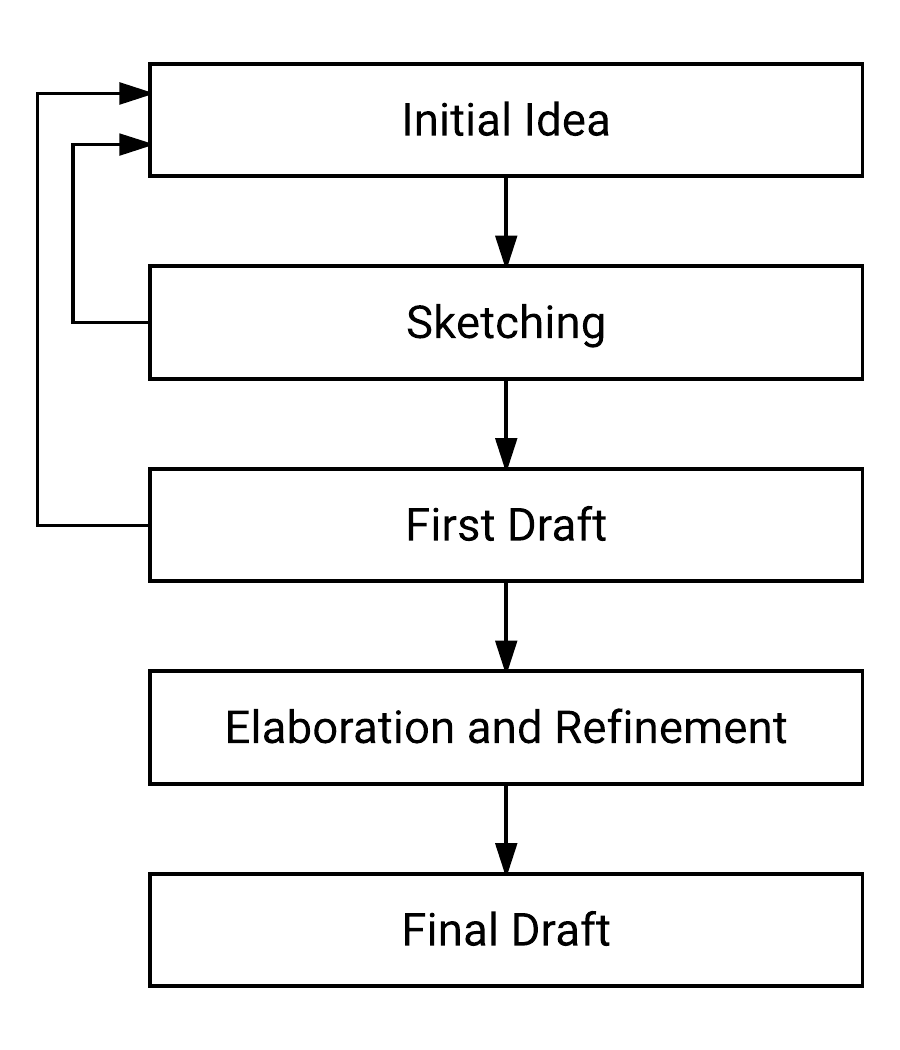
\includegraphics[scale=0.2]{Process_of_Composition}
    \caption{The stages of music composition \citep{bennett1976process}.}
    \label{fig:composing-graph}
\end{figure}

%%need to add gestures in the overview more to define the thingy use of UX in conjunction with the music composition process

There have been several attempts to ease the drafting phase's repetitiveness. To solve this problem, composers along with computer scientists have looked towards \textit{musical metacreation}. This subfield of computational creativity is focused on granting machines the creative capacity to perform musical tasks like composition \citep{pasquier2017an}.

One example of metacreation is found in the case of MorpheuS \citep{herremans2016morpheus}, a music generation system that uses pattern detection techniques to generate music. Alternatively, \citet{kikuchi2016music} attempted to create a music composition tool with recommendations. They utilized gesture interactions, which are methods of communication with computers that use the fingers or hands to execute commands on a touchscreen device \citep{kammer2010towards}. Touch gestures were noted to be a possible medium in the communication of a composer and the computer in the field of music composition \citep{kurtenbach1996gestures}. The tool recommended succeeding notes based on the input provided by the user. 

%% === next main thought should be: given these technologies, what have been the gaps, difficulties encountered as you have seen in the literature???

However, despite these recent advancements, limitations are still present in the existing technologies. In the work of \citet{herremans2016morpheus}, it was admitted that MorpheuS still lacked in terms of musical output and efficiency. The music composition tool created in the study of \citet{kikuchi2016music} was dependent on an existing musical composition because it extracted the rules such as pitch transition and rhythm to predict eventual notes, not from the known strict musical guidelines. This process led to a lack of variety in the generated musical compositions.

\begin{comment}
To solve this lack of variety there were studies that focused on generating musical structures that adhere to a specific theme. Some researchers focused on the structure of happy melodies where they discerned the emotion of happiness in the algorithm by defining explicit rules and using relations to form a generated theme phrase \citep{cao2015automatic}. It was also noted that the researchers created variance in the system by adding a factor of randomness in the pitch generation while still keeping true to the theme of happiness \citep{cao2015automatic}. This yielded computer generated music that was comparable to man-made music \citep{cao2015automatic}.
\end{comment}

Additional studies that desired for computer generated music to be less ``robotic'' focused on the expressive trait of a performer through various elements like emotion \citep{bresin2000emotional}, imitation \citep{miranda2010artificial}, and selection \citep{ramirez2008genetic}. One such study focused on the structure of happy melodies where they discerned the emotion of happiness in the algorithm by defining explicit rules and using relations to form a generated theme phrase \citep{cao2015automatic}. It was also noted that the researchers created variance in the system by adding a factor of randomness in the pitch generation while still keeping true to the theme of happiness \citep{cao2015automatic}. 

From the various algorithms available, most can generate expressive music based on their evaluation metrics \citep{cao2015automatic,bresin2000emotional,miranda2010artificial,de2012playing,ramirez2008genetic,miranda2010artificial} but lacked a usable interface for composers. Computers can help increase the productivity of composers by aiding them during musical composition \citep{velardo2016study}. One such system is Computoser which provided the user with a form based interface that generated music based on choices from multiple selections, and a probability and rule-based algorithm \citep{bozhanov2014computoser}. 

Similar to previous systems, Computoser takes in training data and performs a machine learning algorithm to generate a metacreation model. It was deployed on a website for ease-of-access. However, the interface is form-based and limits the possible compositions (see Figure \ref{fig:computoser-preference}). 

\begin{comment}
One such tool is the Abjad API, an open source software for Python. The tool assists users in creating a musical score by expanding the Python programming language with additional functions that can be used in Python programs \citep{baca2015abjad}. Despite its availability, the tool can only be used by users knowledgeable in the Python programming language and is inaccessible to composers who cannot code. To open computational creativity into a wider audience of composers, there is a need to have a usable interface that does not require any knowledge other than a general understanding of music composition.
\end{comment}

\begin{figure}[H]
    \centering
	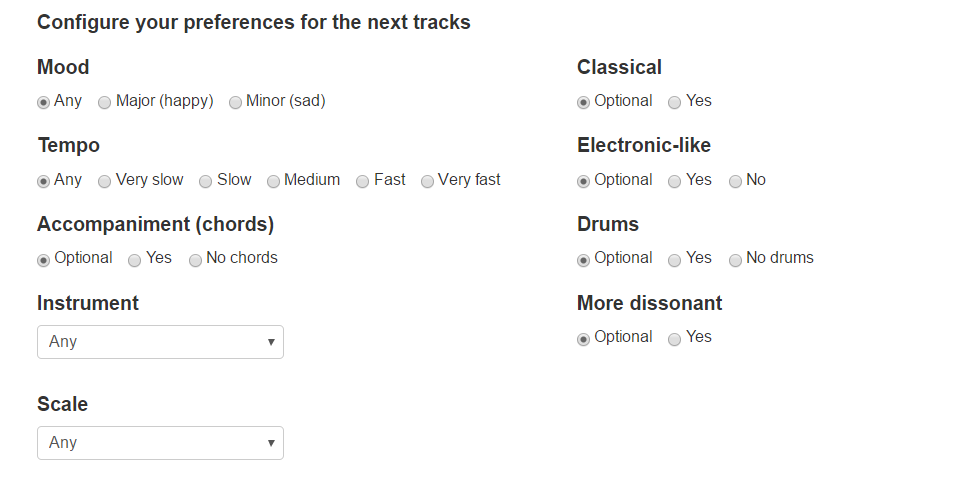
\includegraphics[scale=0.7]{ComputoserSelectionForm}
    \caption{\textit{Computoser} preference selection form \citep{bozhanov2014computoser}.}
    \label{fig:computoser-preference}
\end{figure}

%% === the last main thought of this section should be, summarizing and leading to the research problem that we all intended to solve


The underlying case behind all these findings is figuring out how existing studies on human-computer interactions may augment the current process of music composition. It was found by \citet{brown2017user} that the user experience component was often overlooked when designing interfaces aimed at enhancing the musical composition process. It was suggested in the study of \citep{levitt1992representation} that a computer ``assistant'' that helps the composer during creative lapses would be more beneficial than a system that automatically composes music without any control provided to the user. 

Numerous works on musical metacreation have focused on the algorithms related to music generation and there are limited studies that explore the utilization of human-computer interaction to augment the musical composition process.

\begin{comment}
Although there are already several musical composition tools that aid in the composition of music such as Hyperscore \citep{farbood2004hyperscore} and HARP \citep{camurri1991harp}, the ability to assist composers in a way that it helps them generate ideas are what these systems lack. The graphical user interface of these systems improve the overall user experience of musical composers, but the important problem still remains which is coming up with musical ideas. 
\end{comment}


%% === However, there are possible methods to increase the diversity of the generated music to achieve a level of variety that can be seen as 
   

\section{Research Objectives}
\label{sec:researchobjectives}

\subsection{General Objective}
\label{sec:generalobjective}

To augment the musical composition process by integrating rule-based musical metacreation and gesture interactions

\subsection{Specific Objectives}
\label{sec:specificobjectives}

\begin{enumerate}
	\item To design and develop an application that users can utilize for basic musical composition tasks
    \item To design interactions that will enable users to perform advanced musical composition tasks
    \item To assign gesture interactions for doing compositional tasks in a mobile composition tool
    \item To validate whether the interaction design improves the user experience when using the tool

\end{enumerate}

\section{Scope and Limitations of the Research}
\label{sec:scopelimitations}

The application will be developed for a mobile platform. Through the application, composers can perform basic composition tasks. This includes creating a composition, adding notes, editing notes, and deleting notes. The target instrument of the tool for composition is the piano, due to its popularity.

Only certain musical notation symbols will be available for use in the system. The minimum requirement is to allow composers to perform basic musical notation on a mobile interface.

Composers may perform advanced compositional tasks such as musical metacreation and note transposition. Additionally, composers may also edit multiple notes at the same time by highlighting them. The musical metacreation model will also be limited to a rule-based model.

Given that the application is on a mobile platform, the interactions will be limited to multi-touch gestures that can be handled by this platform. Examples of these gestures are tap, swipe, and flick gestures. The interface will be designed to support finger taps, but a stylus may also be used.

The system aims to provide a dynamic and interactive musical composition experience. To achieve this, it is important that the system's interaction design is tested on actual composers while they accomplish compositional tasks. The target users and testers are composers who have basic knowledge in writing sheet music. These are people who can read and write in musical notation for instrumental music, regardless of the platform or tool. Users are categorized into two (2) levels: newbie, and experienced. Testing will be done with at least 3 composers per level. However, due to the possible schedule limitations of experienced composers, testing with them will be saved for the latter parts of the research when the system has been polished through several iterations of testing. Additionally, to prevent bias, fresh users will be introduced during some iterations of testing. 

The main goal of the proposed solution is not to improve the quality of music produced by the composers, but to aid them in their composition process. It would not replace the composers, as it would only provide suggestions based on the input given by the composer. It is up to the discretion of the composer whether or not to use the metacreated music.

\section{Significance of the Research}
\label{sec:significance}

This study will produce an accessible musical composition tool incorporating concepts from both musical metacreation and human-computer interaction. Given that there are limited studies that use rule-based models, this study will contribute to the emerging field of computational creativity and musical metacreation.

Additionally, the function of the tool will be to augment the musical composition experience of composers. Concepts from both human-computer interaction and music theory will be integrated into the tool to achieve this. Findings from this study will contribute to the knowledge on the process of musical composition, and will provide a background on the integration of human-computer interaction in musical composition.

With the developed system, the improved user experience will help the composer focus more on the composition and the output rather than operating the tool. This would benefit composers that experience creative blocks or have an initial melody in mind, but have no idea how to continue. The tool will aid composers to create music that will still reflect their own style. The personal style of a composer is formed by the culture of the composer. The music created by every composer may reflect their cultural background and personal experiences. This will result in a composition that is a product of an augmented experience but still fully the work of the composer.

Lastly, it is widely known that music has made a great impact on society through the entertainment it brings to people \citep{hawkins2013pac, donnelly2005spectre} and also its therapeutic benefits in common psychological disorders \citep{kemper2005music}. Helping make the composition easier for composers regardless of skill level would allow for better access to music and thereby also granting benefits to society through the several uses of music.

% May problem ako with adding the paradigm of adding focus to Filipino Composers kasi baka mahihirapan tayo mag dagdag pa ng stuff for that, halos lahat ng chapters madadagdagan kapag minention ko Filipino composers dito. Hahanapan nila ng extra proof kung bakit yung tool natin mas makakatulong sa Filipino Composers opposed to other composers

\section{Research Methodology}
This chapter lists and discusses the specific steps and activities that will be performed by the proponent to accomplish the project. 
The discussion covers the activities from pre-proposal to Final Thesis Writing.  It also includes an initial discussion on the theoretical
framework to be followed.

\subsection{Research Activities}

\subsubsection{Planning}
This phase concerns the whole group, with the guidance of the thesis adviser. It involves the formulation of the thesis topic, including the research problem, research objectives, as well as the scope and limitations. This would also include the planning on the approach, and desired output of the study. 

\subsubsection{Review of Related Literature}
Relevant works on musical metacreation, musical composition, and gesture interactions are being studied and synthesized by the group to provide context, and the necessary understanding to perform the study. Works related to musical metacreation are essential to the study due to the insight they provide on how past works have attempted to generate music through different algorithms and modalities. Works on musical composition will be reviewed because they provide a background on the musical theories, as well as the attempts made to augment the musical composition process. Finally, works on gesture interactions will also be reviewed to give context on how gestures play an important role in human-computer interaction as well as how past studies have implemented and studied the said technology in relation to the musical composition process.

\subsubsection{Data Collection}
The group will be doing two kinds of data collection. The first one involves research on music theory and the chord progressions present in music. The information gathered on this will be used for building the model for the system. For the second kind of data, at least three (3) composers will be interviewed to gather data on the musical composition process. Being a study related to human-computer interaction, it is essential that the group understand more about how composers compose music in order to design good interactions to augment the process. Interviews will mainly be done face-to-face, with questions focused on how the composer composes music. Specific details like how the composer transitions from testing a melody to writing it digitally or on paper will be observed. Finally, the composer will also be asked to validate or test a prototype of the proposed system. However before interviews, they will be provided a consent form that would explain what to expect in the interview and testing. They are given the freedom to cancel the interview if they choose to. This will mainly be conducted in the School of Design and Arts building in the De La Salle-College of Saint Benilde. However, depending on the availability of the composers, interviews may also be done in other locations. 

\subsubsection{Interaction Design}
This phase involves design thinking, as it is concerned with the application's user experience and how it would benefit the target users. Interaction design would also include identifying the right placement of user interface (UI) elements, as well as the right methods to interact with them (i.e. gestures and taps). The data gathered from the observations and interviews with composers would provide the insight necessary to make design decisions that would result in an interaction that benefits the users. Design artifacts like affinity diagrams and user personas would be used to represent these users in a collected, yet organized form. This will be done repeatedly, and will be validated through more interviews and tests. This is to ensure that the proposed solution would integrate seamlessly with the musical composition process.

% This phase is all about design thinking. It is concerned with the user experience design of the solution and how it can benefit the target users, composers. The data gathered during data collection, specifically the interviews with the composers, will be maximized in this phase since it would provide the insight necessary to understand how they compose. This will be done repeatedly, with validation, to ensure that the solution will integrate seamlessly with the musical composition process.

\subsubsection{Implementation}
Once the interaction design has been laid out and validated, the actual system can then be implemented. The system will be in the form of a mobile application in the iOS platform. It will be optimized for iPads, due to its larger screen size compared to regular phones. The validated interaction design formulated during the previous phase would be implemented in the application. This phase would involve iterations of more testing and development to continuously gather user experience and interaction data that would help improve the application's design.

% Included in this phase will be the necessary testing in order to ensure the model's correctness, accuracy, and usability.

\subsubsection{Experiment Design}
 In order to assess the effectiveness of the developed system, experiments will have to be conducted in every iteration throughout the study. However, these experiments have to be designed so that they could effectively measure interaction and user experience. With that said, common user experience metrics like KLM-GOMS, and Fitts Law will be used and measured using CogTool. Additionally, testing will be done with at least three (3) composers per level (newbie and experienced), totaling to at least six (6) composers. Before the testing, they will be given a consent form indicating the ethical considerations of the research. At this point, they may choose to opt out of the testing, or continue with it. If they continue, they will be asked to perform a set of tasks that would help the researchers identify any flaws or issues that can be improved in the user experience and interaction design. Note that these composers may change in between iterations to prevent bias and inaccurate results. 

% In order to assess the effectiveness of the developed system, experiments will have to be conducted throughout the course of this study. However, in order for the results to be as accurate as possible, the experiments have to be designed accordingly so that they measure interaction and user experience. Research will be done on how to effectively measure user experience metrics and system interaction. This will involve creating use cases, test scenarios, and identifying the pains and gains of the users. Testing will be done with at least three (3) composers per level (newbie and experienced), totaling to at least six (6) composers. Before the testing, they will be given a consent form indicating the ethical considerations of the research. At this point, they may choose to opt out of the testing, or continue with it. 

\subsubsection{Results Analysis}
This activity will include analysis on the findings gathered during review of related literature, data collection, and experimentation. It involves performing quantitative and/or qualitative analyses on the gathered data and review them in order to improve the system. This will also involve creating use cases, test scenarios, and identifying the pains and gains of the users. The privacy of the respondents will also be maintained, with any information about them including their name, age, or working experience hidden. Any results or comments received from the users will only be used for this study. They will not be released or publicized in any form. The researchers will be implementing a methodology called \textit{user personas} to represent users without having to compromise their privacy.

\subsubsection{Documentation}
The documentation will be done during the entire study. This will include documentation on all the activities performed, as well as their results and discussion.

\subsection{Calendar of Activities}
Table \ref{tab:timetableactivities} shows a Gantt chart of the activities.  Each bullet represents approximately
one week worth of activity.

%
%  the following commands will be used for filling up the bullets in the Gantt chart
%
\newcommand{\weekone}{\textbullet}
\newcommand{\weektwo}{\textbullet \textbullet}
\newcommand{\weekthree}{\textbullet \textbullet \textbullet}
\newcommand{\weekfour}{\textbullet \textbullet \textbullet \textbullet}

%
%  alternative to bullet is a star 
%
\begin{comment}
   \newcommand{\weekone}{$\star$}
   \newcommand{\weektwo}{$\star \star$}
   \newcommand{\weekthree}{$\star \star \star$}
   \newcommand{\weekfour}{$\star \star \star \star$ }
\end{comment}

\begin{comment}
\begin{table}[ht]  %t means place on top, replace with b if you want to place at the bottom
\centering
\caption{Timetable of Activities} \vspace{0.25em}
\begin{tabular}{|p{2in}|c|c|c|c|c|c|c|c|c|} \hline
\centering Activities-2017 & May & Jun & Jul & Aug & Sep & Oct & Nov & Dec \\ \hline
Planning     & ~~\weekone~ & \weekone~~~ & \weekone~~~ & \weekone~~~ & & & & \\ \hline
Review of Related Literature & ~~\weektwo & \weekfour & \weekfour & \weekone~~~ &  &  & & \\ \hline
Data Collection     &   &  & ~~~\weekone & \weekfour & \weekone~~~ &  &  &\\ \hline
Interaction Design    &   &  &  & \weekfour & \weektwo~~ &  &&  \\ \hline
Implementation      &   &  &  &  & \weekfour & \weekfour & \weektwo~~ &\\ \hline
Experiment Design &   &  &  &  &  & ~~\weektwo & \weekfour & \\ \hline
Results Analysis &  &  &  &  & & &  & \weektwo~~ \\ \hline
Documentation & ~~~\weekone  & ~~~\weekone & ~~~\weekone & ~~~\weekone & ~~~\weekone & ~~~\weekone & ~~~\weekone & \weekone~~~ \\ \hline
\end{tabular}
\label{tab:timetableactivities}
\end{table}

\begin{table}[ht]  %t means place on top, replace with b if you want to place at the bottom
\centering
\begin{tabular}{|p{2in}|c|c|c|c|c|c|c|c|c|} \hline
\centering Activities-2018 & Jan & Feb & Mar & April & May & Jun & Jul & Aug \\ \hline
Planning     & ~\weekone~~  & \weekone~~ &  &  & \weekone &  &  & \\ \hline
Review of Related Literature &  & & & ~~\weektwo & \weektwo~~ & & & \\ \hline
Data Collection     &   &  &  & & &  &  &\\ \hline
Interaction Design    &  & \weekfour & \weekfour & & &  &&  \\ \hline
Implementation      &   &  & \weekfour & \weekfour &  & &  &\\ \hline
Experiment Design &   &  &  & \weekfour & \weektwo~~ &  & & \\ \hline
Results Analysis & ~\weekthree & \weekfour & &  & \weekfour & \weekfour &  &  \\ \hline
Documentation & ~~~\weekone  & ~~~\weekone & ~~~\weekone & ~~~\weekone & ~~~\weekone & ~~~\weekone & \weekfour & \weektwo~~ \\ \hline
\end{tabular}
\label{tab:timetableactivities2}
\end{table}
\end{comment}

\begin{landscape} % Landscape page
\begin{table} [!htbp]  
\centering
\caption{Timetable of Activities} \vspace{0.25em}
\begin{tabular}{|p{1.1in}|c|c|c|c|c|c|c|c|c|c|c|c|c|c|c|c|c|} \hline
  \centering 2017-2018 & May & Jun & Jul & Aug & Sep & Oct & Nov & Dec & Jan & Feb & Mar & Apr & May & Jun & Jul\\ \hline
  Planning     & ~~\weekone~ & \weekone~~~ & \weekone~~~ & \weekone~~~ & & & & & ~\weekone~~  & \weekone~~ &  &  & \weekone &  & \\ \hline
  Review of Related Literature & ~~\weektwo & \weekfour & \weekfour & \weekone~~~ &  &  & & &  & & & ~~\weektwo & \weektwo~~ & & \\ \hline
  Data Collection     &   &  & ~~~\weekone & \weekfour & \weekone~~~ &  &  & &   &  &  & & &  &  \\ \hline
  Interaction Design    &   &  &  & \weekfour & \weektwo~~ &  & &  &  & \weekfour & \weekfour & & &  & \\ \hline
  Implementation      &   &  &  &  & \weekfour & \weekfour & \weektwo~~ & &   &  & \weekfour & \weekfour &  & &  \\ \hline
  Experiment Design &   &  &  &  &  & ~~\weektwo & \weekfour & &   &  &  & \weekfour & \weektwo~~ &  & \\ \hline
  Results Analysis &  &  &  &  & & &  & \weektwo~~ & ~\weekthree & \weekfour & &  & \weekfour & \weekfour & \\ \hline
  Documentation & ~~~\weekone  & ~~~\weekone & ~~~\weekone & ~~~\weekone & ~~~\weekone & ~~~\weekone & ~~~\weekone & \weekone~~~ & ~~~\weekone  & ~~~\weekone & ~~~\weekone & ~~~\weekone & ~~\weektwo & \weekfour & \weekfour\\ \hline
\end{tabular}
\label{tab:timetableactivities}
\end{table}
\end{landscape}



               %-- includes LaTeX source file for Chapter 1: Research Description
                                  %-- your job: **EDIT THIS FILE** to indicate your own research description

%%%%%%%%%%%%%%%%%%%%%%%%%%%%%%%%%%%%%%%%%%%%%%%%%%%%%%%%%%%%%%%%%%%%%%%%%%%%%%%%%%%%%%%%%%%%%%%%%%%%%%
%
%   Filename    : chapter_2.tex 
%
%   Description : This file will contain your Review of Related Literature.
%                 
%%%%%%%%%%%%%%%%%%%%%%%%%%%%%%%%%%%%%%%%%%%%%%%%%%%%%%%%%%%%%%%%%%%%%%%%%%%%%%%%%%%%%%%%%%%%%%%%%%%%%%

\chapter{Review of Related Literature}
\label{sec:relatedlit}
\begin{comment}
then for team MusicG my suggested columns would be 
2.1 Authors | Focus (if melody, chord, progression, sequence) | Model (what math formula or name did they use no need to put formula sa table) 
2.2 Authors | Name of Tool | Platform | Input Type | Algorithm (what they used to generate sequences)
2.3 Authors | Name of Tool | How many testers | Comments  and other  reported findings
Testing Someting
\end{comment}

This chapter discusses the features, capabilities, and limitations of existing research, algorithms, or software that are related/similar to the study.

\section{Mathematical Analysis of Music and its Melodies}
This section provides an analysis on different works towards modeling music and melody mathematically. Because of the musical nature of this study, it is important to understand the terms used in music and how past studies have made steps to mathematically represent music and its elements.

\citet{loy2011musimathics} defines music as a creative form of art whose medium is sound. It includes several elements (e.g., note, pitch, rhythm, etc.) which can be represented mathematically. One such element is melody. The melody plays an important part in music \citep{unehara2001composition,unehara2005music} as it is the sequence of notes that define the sound of music \citep{ryynanen2008automatic}. 

The melody will most likely make the most impact on the listener \citep{jarret2008music}. These succession of notes usually define the body or general idea of a composition through the form it takes in a musical framework \citep{jarret2008music}. Whether this form contains quick tempos that provoke the listener into motion or a slow tempo leaving the listener relaxed, it is important for a composer to add melodies that can bring the composition to life \citep{jarret2008music}. 

% The listener will more than likely be impacted the most by the melody of the composition \citep{jarret2008music}. These succession of notes usually define the body or general idea of a composition through the form it takes in a musical framework \citep{jarret2008music}. Whether this form contains quick tempos that provoke the listener into motion or a slow tempo leaving the listener relaxed, it is important for a composer to add melodies that can bring the composition to life \citep{jarret2008music}. 

\citet{poliner2007melody} provided a more musicological definition of melody, which is the single pitch sequence that a listener would recognize to be the ``essence'' or the ``soul'' of the composition being listened to. This definition was later supported in the study of \citet{salamon2012melody}, where they attempted to extract the melody from music signals by identifying the most significant pitch in a composition. 

Both \citet{poliner2007melody} and \citet{salamon2012melody} borrowed the mathematical representation of melody that was provided by \citet{goto2004real} in his earlier study. \citeauthor{goto2004real} represented melody through a predominant-F0 estimation method, or what he called \textit{PreFEst}, where F0 denotes the fundamental frequency. In this method, the melody is identified by finding the strongest, or most dominant harmonic structure within specific regions of the audio signal. 

\begin{comment}
However, according to \citet{dannenberg1993music}, representing music mathematically is difficult as there are some elements involved that cannot be represented by math, like the emotion involved when playing music. Despite this, research has gone into analyzing the elements of music that can be represented mathematically, such as pitch, which has a key role in music as it determines how ``high'' or ``low'' a note would sound.
\end{comment}

On the other hand, \citet{dorfler2001time} links music signals to Gabor analysis, a method of analyzing music by separating it into segments referred to as frames \citep{gabor1946theory}. Given that music has many high-level and low-level music features that can be represented in the mathematical aspect, \citet{dorfler2001time} relates how music is very similar to a Hilbert Space in terms of digital signal processing. This can be modeled into a set of energy signals that contains many features that she considers to belong in a space of square-integrable functions \begin{math} {L}^2 (\mathbb{R}),\mathbb{R} \rightarrow  \mathbb{C}  \end{math}. Following this, \citet{dorfler2001time} mentions that such spaces which are capable of containing complex set of features are usually infinite in form. However, she mentions that though music may contain such set of features, it is not infinite but rather it is continuous in form. To accommodate this, she proposed a modification of the existing model that accommodates the limitations in finiteness.

\begin{comment}
\begin{equation}
\label{eq:1}
l^2(\mathbb{Z}):=\left\{f:\mathbb{Z}\rightarrow\mathbb{C}\sum_{n=-\infty}^\infty|f(n)|^2<\infty \right\}
\end{equation}
Test1
\begin{equation}
\label{eq:2}
(f*g)(n)=\sum_m f(m)g(n-m)
\end{equation}
\end{comment}

She introduces that music is usually measured in length \begin{math}L\end{math} as members of the complex vector space \begin{math}\mathbb{C}^L\end{math} where finite sequences are treated as period sequences in forms of what she introduces as \textit{circular extensions} of the said signals coming from \begin{math}\mathbb{Z}_L = \mathbb{Z} mod L\end{math} \citep{dorfler2001time}. 

This was supported by the earlier work of \citet{fucks1962mathematical} where he focused on analyzing the statistical aspects of music, specifically the frequency distribution of the pitch in music present from 1500 - 1960. This time, he represented the such sequences in what he calls \textit{kurtosis} (\textit{K}), that is defined as the measure of the sharpness of the peak in frequency distributions. In retrospect, the length of digital signals introduced by \cite{dorfler2001time} are similar in meaning to the frequencies measured by \cite{fucks1962mathematical}. 

\begin{comment}
\begin{equation}
\label{eq:3}
K = \frac{\mu^4}{\sigma^4}
\end{equation}

\begin{equation}
\label{eq:4}
\mu_v = \sum_x(x-\overline{x})^v\cdot p_x
\end{equation}

\begin{equation}
\label{eq:5}
\overline{x} = \sum_x\cdot p_x
\end{equation}
\end{comment}

\citet{voss1978noise} initiated the study on the spectral density of music, where spectral density is defined as a function that determines the strength of the energy of a signal \citep{stoica1997introduction, martin2001noise}. In their study, \citeauthor{voss1978noise} found that music that exhibited a spectral density of $\frac{1}{f}$ noise, where \textit{f} is the frequency, was particularly pleasing to hear. This was mainly due to how the certain frequency was similar to that of human communication. The other spectral density that was observed, $\frac{1}{f^2}$ noise, was considered less pleasant \citep{gunduz2005mathematical}, and too correlated \citep{voss1978noise,nettheim1992on}. 

\citet{buxton1978the} investigated the possibility of modeling music as data structures in what he calls \textit{hierarchies}. \citeauthor{buxton1978the} defined a \textit{hierarchy} as a structure that contains either a single note, or another \textit{hierarchy}. He observed that a musical composition can be separated into chunks and be played separately. Within these said chunks could be other smaller chunks or up to just a single note. By treating music as \textit{hierarchies} or chunks, the music could have multiple levels where whenever a level is played, all the levels beneath it would also be played. The composer would have the ability to choose smaller chunks or lower levels of the music to be able to play a certain part. This system of representing music as \textit{hierarchies} was also supported by \citet{brinkman1984data} in his study with the use of linked lists. 

The same ideology was also present in the later study of \citet{bozhanov2014computoser}. In this study, music was modeled as a set of rules. A composition is considered as a structure, with its own properties like rhythm, meter, scale, etc. Similarly, the study of \citep{schulze2011music} also represented music using rules, but more specifically, Markov chains. The composition is modeled using probabilistic automata with the states as its notes.

Shown in Table \ref{tab:rsotmaomaim} is a summary of the reviewed works and a comparison of their focus and model.

\begin{landscape} % Landscape page
\begin{table} [!htbp]  

        \captionof{table}{Related Studies on the Mathematical Analysis of Music and its Melodies} \label{tab:rsotmaomaim} 
   \vspace{0.20cm}    
        \begin{tabular}{|p{5cm}|p{5cm}|p{5cm}|p{5cm}|} %{|l|l|l}
        \hline 

       Authors & Focus & Theory/Principle & Contributions/Details \\ \hline
       
       \citet{goto2004real, salamon2012melody, poliner2007melody} & Melody & Fundamental Frequency (F0) & Melody is the most dominant harmonic structure \\ \hline
       
       \citet{dorfler2001time} & Music as a digital signal & Gabor analysis \& Hilbert space & Music contains features that are infinite in form, but it is still continuous \\ \hline
       
       \citet{fucks1962mathematical} & Pitch & Kurtosis and Frequency Distribution & The pitch can be analyzed in terms of peaks in frequency distributions \\ \hline
       
       \citet{voss1978noise, nettheim1992on, gunduz2005mathematical} & Frequency, Pitch \& Melody & Spectral Density & Music generally exhibits a spectral density of $\frac{1}{f}$ noise \\ \hline
       
       \citet{buxton1978the, brinkman1984data} & Music & Hierarchies or Chunks & A composition is a structure that can be separated into substructures \\ \hline
       
       \citet{bozhanov2014computoser} & Music & Rule-based algorithm & A composition can be modeled using a structure with rules and properties \\ \hline
       
       \citet{schulze2011music} & Music & Markov chains and Probabilistic automata & A composition can be represented as a set of states \\ \hline
       
        \end{tabular}
\end{table}
\end{landscape}


\section{Musical Composition \& Recommendation Systems}
This section contains a review of research papers that discuss systems that produced musical compositions with the aid of various algorithms.

Musical composition systems that attempted to augment the composition process have already been developed in the past. \citet{eigenfeldt2010realtime} generated music through their system that makes use of Markov models, a method of generating sequences or melodies by deriving features from a provided corpus. However, this also resulted in an inability to generate a deeper, or a varied structure of music, which was also expressed in the earlier study of \citet{ames1989markov}. 

% The advantage of Markov models were that they did not need to follow any rules. 

\citet{herremans2016morpheus} developed MorpheuS which is a system that generates music with the use of tension profiles that are computed from a template of a musical piece. The system uses an optimization approach which avoids the recursive behavior of Markov models during pattern finding to avoid the use of non-standard hierarchical models which lack efficiency \citep{herremans2016morpheus}. 

\begin{comment}
There are other approaches which yield more efficient results \citep{damlen1999gibbs}. COSIATEC and SIATECCompress are two greedy compression algorithms used by MorpheuS that find patterns in a given template piece.
\end{comment}

% Another similar system is SuperWillow which was developed in the study of \citet{schulze2011music}. It uses symbolic music as the representation of partially composed music. They conducted a partial Turing test wherein respondents were asked to identify which of the two given musical compositions was composed by a human being. 38\% of the respondents incorrectly identified the computer-generated musical composition as a human composition. The SuperWillow uses LearnPSA algorithm which generates prediction suffix trees that is converted to PSA. Probably approximately correct learning model (PAC) prompted the PSA algorithm. After composition analysis, the objects generated are then used in order to compose or imitate music using the training data. Distribution sampling is used in order to generate music instead of calculating the probable sequence of notes.

% Another similar system is SuperWillow which was developed in the study of \citet{schulze2011music}. It uses symbolic music as the representation of partially composed music. The SuperWillow uses LearnPSA algorithm which generates prediction suffix trees that is converted to PSA. Probably approximately correct learning model (PAC) prompted the PSA algorithm. After composition analysis, the objects generated are then used in order to compose or imitate music using the training data. Distribution sampling is used in order to generate music instead of calculating the probable sequence of notes.

Another similar system is SuperWillow which was developed in the study of \citet{schulze2011music}. SuperWillow takes in musical data in the form of MusicXML. The data is then used to generate Markov chains and probabilistic automatons to model musical elements. After composition analysis, the objects generated are then used in order to compose or imitate music similar to the training data. Distribution sampling is used in order to generate music instead of calculating the probable sequence of notes.

\citet{kikuchi2014automatic} approached musical metacreation using a genetic algorithm to generate melody. The approach used N-gram models to represent rhythm and pitch in each melody block to use in the algorithm. In order to produce melodies, musical features are likened to human genes, which contain different properties. The first part of the process involves random generation of initial individuals that are based on rhythm, pitch, and chord progression. Fitness calculation will then be done to determine which individuals have similar musical features for the crossover. The parent individuals will be used to generate new individuals, repeatedly.

% A genetic algorithm was also used the Composition in Genetic Approach (CONGA) \citep{tokui2000music}. The system takes in a fitness score or evaluation in order to generate a better rhythm. It suggests that people have various preferences based on their personal fitness scores, which can be subjective. It uses both the genetic algorithm and genetic programming which complements each other in creating structured rhythm. Every time the user submits a fitness evaluation, the genetic algorithm and genetic programming starts to improve or sustain the rhythm produced based from their input and returns a rhythm which is needed to be evaluated by the user again.

A genetic algorithm was also used the Composition in Genetic Approach (CONGA) \citep{tokui2000music}. The system takes in a fitness score or evaluation in order to generate a better rhythm. Every time the user submits a fitness evaluation, the genetic algorithm and genetic programming starts to improve or sustain the rhythm produced based from their input and returns a rhythm which is needed to be evaluated by the user again.

The study of \cite{geis2008creating} developed a system that used Ant Colony Optimization (ACO) for the generation. ACO also depended on multiple iterations of training similar to previous studies that used genetic algorithms \citep{tokui2000music,kikuchi2016music}. It was believed that composers sometimes broke musical rules in their compositions. This study attempted to model that behavior with how ants followed certain pheromones while searching for food, hence the ACO algorithm. However, the study's limitation was that it did not include a Graphical User Interface (GUI) to allow for real time input \citep{geis2008creating}.

% The study of \cite{geis2008creating} developed a system that used Ant Colony Optimization (ACO) for the generation. ACO also depended on multiple iterations of training similar to previous studies that used genetic algorithms \citep{tokui2000music,kikuchi2016music}. It was remarked in the study that there were great composers that broke musical rules, and they wanted to mimic those sudden changes through the ACO algorithm which mimicked how ants followed certain pheromones while searching for food \citep{geis2008creating}. Despite the music generated from the system being satisfactory to the musical criteria presented by the researchers, a suiting Graphical User Interface (GUI) was not developed for real time input \citep{geis2008creating}.

Aforementioned systems focused on musical metacreation, leaving aside user experience, resulting in a lack of interaction. Hyperscore, developed by \citet{farbood2004hyperscore}, focused on user experience by designing an appropriate graphical user interface for the musical structure. The idea behind Hyperscore was to allow people to compose short melodies with minimal expertise in musical composition.  \citeauthor{farbood2004hyperscore} believed that the new method of interaction allowed users to have an expressive way of shaping musical direction.

\citet{kikuchi2016music} supported the idea of musical composition with interaction. They developed a music composition tool that used the Microsoft Surface Pro 3 and the Surface Pen, which enabled the use of gestures for its interactions. It provides users possible pitches to continue writing the composition that is being written. The system involves extraction of pitch transition and rhythm from a musical piece provided by the user as input. Those features are used to generate the recommended pitches and present them to the user in real time. They are then stored in a local SQLite database and searched every time the system is trying to find the right pitch or pitches to recommend to display.

Another system that included a user interface was Computoser, developed by \citet{bozhanov2014computoser}. Similar to previous studies, it uses a rule-based approach but includes probabilistic characteristics in the algorithm for generating music. The rules in the system were based on music theory and with the help of some experts \citep{bozhanov2014computoser}. As seen in Figure \ref{fig:computoser-preference}, the system enables the user to adjust the weights in the preferences with which the music is generated. The result is a composition based to the choices the user made and can be immediately played in the web browser through a media player present in the website as seen in Figure \ref{fig:computoser-media}. 

\begin{figure}[H]
	\centering
	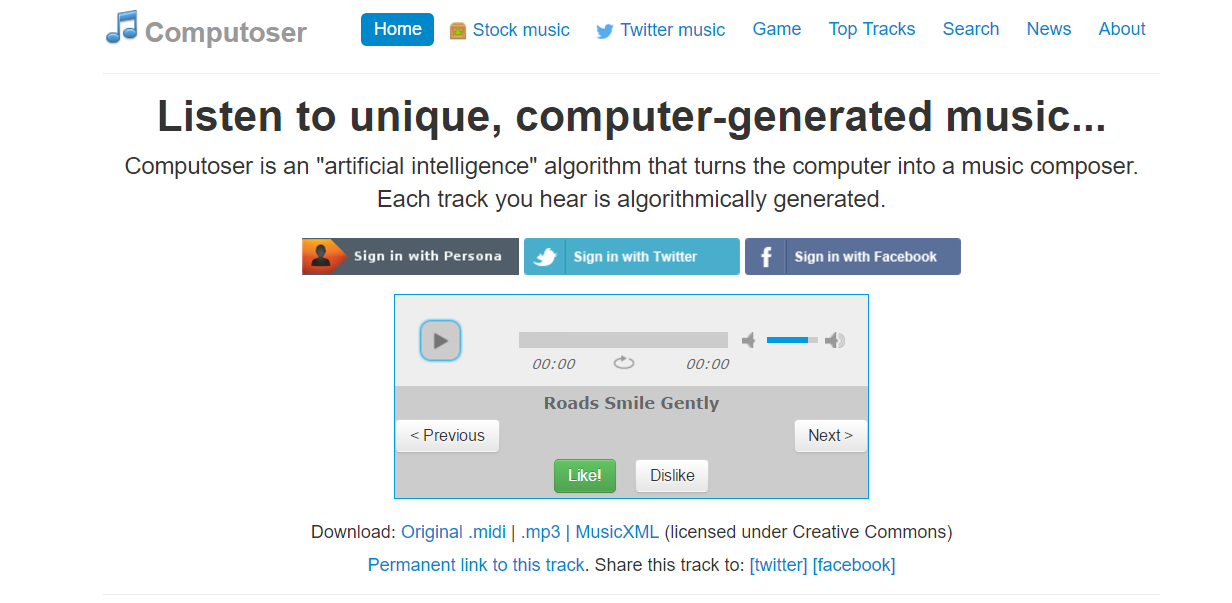
\includegraphics[scale=0.5]{ComputoserMediaPlayer}
    \caption{\textit{Computoser} media player \citep{bozhanov2014computoser}.}
    \label{fig:computoser-media}
\end{figure}

\begin{comment}
Another way to improve upon the process of musical composition is through focusing on what feels natural to the target users. Composers and musicians also feel with their body when composing music through instruments \citep{de2012playing}. In recent years, the use of touch interfaces have proven to feel more natural than using external input devices like the mouse \citep{travis2014comparative}. The use of gesture interactions through modern innovations like the touch screen is both an intuitive and interaction focused approach for a system \citep{epps2006a}. It is also mentioned in the study of \cite{travis2014comparative} that despite the general acceptance of the public with the innovation of touch, there are still facets of the technology that can be improved upon for the overall performance and usability of the touch screen \citep{travis2014comparative}.
\end{comment}

% FORMAT FOR A NEW ROW IN 2.2 : \citet{} & 1 & 2 & 3 & 4 \\ \hline

\begin{landscape} % Landscape page
\begin{table} [!htbp]  
\label{tab:rsomcrtas}        
        \captionof{table}{Related Studies on Musical Composition \& Recommendation Tools and Systems}
   \vspace{0.20cm}    
        \begin{tabular}{|p{3cm}|p{4cm}|p{3cm}| p{5cm} | p{5cm}| } %{|l|l|l}
        \hline 
       Authors & Name of Tool & Platform & Input/Modality & Algorithm \\ \hline
       
       \citet{ames1989markov,eigenfeldt2010realtime} & NA & NA & MIDI files & Markov models \\ \hline
      
       \citet{herremans2016morpheus} & MorpheuS & NA & Template piece & Tension profiles \\ \hline
       
       \citet{camurri1991harp} & HARP & NA & Source composition/piece & Networks\\ \hline
       
       \citet{tokui2000music, kikuchi2014automatic} & CONGA; NA & PC; NA & Fitness Score; NA & Genetic Algorithm with Genetic Programming; Genetic Algorithm with N-grams\\
        \hline
        
        \citet{kikuchi2016music} & Music Composition with Recommendation & Tablet (Microsoft Surface Pro 3) & Touch with the use of Surface Pen & Database of Features \\ \hline
        
        \citet{bozhanov2014computoser} & Computoser & Web & Form-Based & Hybrid Rule-Based, Probability Driven Algorithm \\
        \hline
        
        \citet{geis2008creating} & NA & PC & Length of melody \& Set of allowed pitches & Ant Colony Optimization \\
        \hline
      
        \end{tabular}
\end{table}
\end{landscape}

\section{Music Generation and Evaluation}

% In the current metrics of computer generated music evaluation, the objective is to make the music feel “expressive” wherein the sound of the music does not sound monotonous and complies with the unique changes every composer adds to their piece \citep{de2002ai}. It is where the music generated feels human, where it has these subtle differences in tempo, pitch, timbre, and volume \citep{bresin2000emotional}. Studies have found that monotony makes for a piece that will leave the human brain's neuron's fire rate decrease because of habituation \citep{baars1993cognitive} therefore creating a dull musical experience. The excitement of change can increase the rate of how a brain’s neurons fire leaving the mind filled with activity \citep{de2012playing}.

In the current metrics of computer generated music evaluation, the objective is to make the music feel “expressive” wherein the sound of the music does not sound monotonous and complies with the unique changes every composer adds to their piece \citep{de2002ai}. It is where the music generated feels human, and has these subtle differences in tempo, pitch, timbre, and volume \citep{bresin2000emotional}. Expressiveness is a criterion for music and is defined as how close a computer-generated melody is to its human counterpart \citep{de2002ai}. Evaluation metrics range from how a generated piece not only conforms to the musical metrics and standards, but also to the change in dynamics that are found within songs composed to evoke certain emotions within the audience by the artist \citep{bresin2000emotional}. 

% Expressiveness is a criterion for music and is defined as how close a computer-generated melody is to its human counterpart \citep{de2002ai}. Evaluation metrics range from how a generated piece not only conforms to the musical metrics and standards, but also to the change in dynamics that are found within songs composed to evoke certain emotions within the audience by the artist \citep{bresin2000emotional}. In the field of computing, these systems that generated music purely using the context of the data input or through some extra input by the user were referred to as computer systems for expressive music performance (CSEMP) \citep{miranda2010artificial}. 

The TempoExpress system aimed to produce expressive music from monotonous music recordings \citep{grachten2006a}. The system used a principle called case-based reasoning (CBR), where it used cases as knowledge for the computer to refer to when generating a musical piece. CBR was used because of how the nature of music can differ with every piece. It can contain all the specific changes in each musical piece \citep{de2012playing}. The evaluation was done through a survey of 92 participants and then run through a performance measure \citep{grachten2006a}.

Saxex, a system that generates expressive saxophone jazz solos, also uses CBR. CBR performed well to help the system deal with the dynamics, rubato, vibrato, articulation, and attack of the notes in the jazz solo generated by the system \citep{arcos1998saxex}. The resulting melodies where then run through a spectral modeling synthesis (SMS) technique then analyzed whether the music was expressive or not \citep{arcos1998saxex}.

An Imitative Multi-Agent Perform (IMAP) was used in the study of \citet{miranda2010artificial}. The IMAP mimics how people listen to music and use it as inspiration for their own composition. The system used rules to evaluate given music, and only used the highest rated music as inspiration. It was then tested using certain algorithms to evaluate its success when generating melodies after training \citep{miranda2010artificial}.

% There are also systems wherein evaluation was not strictly done after a melody was generated. An Imitative Multi-Agent Performer (IMAP) runs through the cycle of evaluating one another then composing their own music after reflecting on the music previously listened to that had a high rating \citep{miranda2010artificial}. This system mimics how people listen to music and use it as their inspiration for future work. The evaluation of an agent within the system is determined with a set of rules for easier control over the parameters in rating different kinds of expressive music \citep{miranda2010artificial}. IMAP was then tested for certain categories and run through algorithms to evaluate its success in generating melodies after training \citep{miranda2010artificial}. 

% There is a similarity between IMAP system and the study of \citet{dahlstedt2006musical}. Both used multiple agents for musical metacreation. The main difference between the two is \citeauthor{miranda2010artificial} used the agents for evaluation, while \citeauthor{dahlstedt2006musical} used the agents for the actual metacreation. However, the study's research objectives were not met due to the agents' immaturity \citep{dahlstedt2006musical}.

% There is a similarity between IMAP system and the study of \citet{dahlstedt2006musical} where multiple agents where used to do certain tasks in generating a system. These multi-agents differ in the individual tasks each agent performs where in the IMAP system of \citet{miranda2010artificial}, each agent evaluated and performed within the community of agents while the agents in \citet{dahlstedt2006musical}'s system were splitting the tasks in the process of music creation. It was remarked how the discipline of agents was still in its developing stage since their system was not able to achieve the research objectives at that time \citep{dahlstedt2006musical}.

% MorpheuS, developed in the study of \citet{herremans2016morpheus} makes use of an efficient search algorithm called variable neighborhood search which generates polyphonic music with themes and tension profiles. Making use of tension profiles are useful in the context of game of film music. The results of the system turns out to be favorable since it has been used in different events around the world. Although the results turn out to be favorable, the researchers plan to further improve the overall efficiency of the system. Other improvements in the system include the quality of musical output by imposing more restrictions regarding the playability and the analytical properties of a style of music.

MorpheuS, developed in the study of \citet{herremans2016morpheus}, was tested by playing the results of the system in different musical events around the world. Although the results turned out to be favorable, the researchers plan to further improve the overall efficiency of the system. Other improvements in the system include the quality of musical output by imposing more restrictions regarding the playability and the analytical properties of a style of music.

In the study of \citet{schulze2011music}, SuperWillow was evaluated through a partial Turing test. Respondents were asked to identify human compositions versus computer-generated compositions. It was found that 72\% of the respondents either could not tell the difference between the composition composed by the computer and the human, or preferred computer-generated compositions over human compositions.

\citet{kikuchi2016music} performed testing on users with little experience in musical composition. They compared their system with another composition tool that was a Piano-roll type. It was found that their system allowed for more variety in compositions compared to the other system. Despite this, the system was still limited to the pitch transitions and rhythm of the training input provided \citep{kikuchi2016music}.

% \citet{kikuchi2016music} tested the system they developed by letting a user that has limited experience in composing music use their software and a composition system which was Piano-roll type. Compared with the Piano-roll system, their system produced musical compositions with more variety. However, their system is limited to the pitch transitions and rhythm of the provided musical piece. The originality of the musical composition can be an issue when it comes to generated music \citep{farbood2001hyperscore}.

% In the system of \cite{geis2008creating}, an ACO algorithm was used to generate music. The algorithm was similar used natural occurrences similar to that of genetic evolution. It was evaluated through rules in every stage of developing the composition. In its melody creation stage, smoothness, contour, tendency tone resolution, tone color, and pitch of the final note in the melody was evaluated \citep{geis2008creating}. In the baroque harmonization stage, chord arrangement, voice distance, voice leading, harmonic progression, smoothness, and chord resolutions were factors in the final piece \citep{geis2008creating}. These rules were enforced along with weights and parameters that the ACO algorithm follows.

\citet{yiiksel2011automatic} also developed a software that utilized a genetic algorithm. Their system generated notes using a genetic algorithm with recurrent neural networks. The algorithm used properties such as note, octave, and duration. Although it was only tested by the researchers, it was found that the metacreated music was only viable after a number of evolutions have been made. 

% Another software that revolves around the genetic algorithm was developed by \citet{yiiksel2011automatic}. They developed a system where the notes are generated through a genetic algorithm alongside with recurrent neural networks hence, removing the need of interaction. The properties of each gene used in the genetic algorithm are the note, octave, and duration. Music produced from their software is seen viable only after a number of evolutions or generations have been made.

Alternatively, in the study of \citet{birchfield2003generative}, a genetic algorithm was used with consideration for musical emotion, meaning, and form. The testing found that average listeners found the metacreated music to be interesting. On the other hand, a focused intensity was noticed by the experts due to the shifting rhythms, gestures, and phrasing \citep{birchfield2003generative}. Although experts also noted that the music contained some idle sections. This affected the emotion evoked by the music \citep{birchfield2003generative}.

% A generative model with the consideration of musical emotion, meaning, and form was also developed with the genetic algorithm. \citet{birchfield2003generative} created this generative model that revolved around various rules in composing music which includes the theory by Leonard Meyer which focuses on structuring music to be effective in portraying emotion. The results from the average and expert listeners did not vary much from each other. Average listeners found the music produced by the algorithm to be interesting and assessed it to be having a local variation. On the other hand, a focused intensity was noticed by the experts which was due to the shifting rhythms, gestures, and phrasing \cite{birchfield2003generative}. Some idle sections were also noticed by the experts which could result in destroying the momentum of emotion being portrayed by the music.

%\newpage
%\afterpage{\clearpage}

\begin{landscape} % Landscape page
\begin{table} [!htbp]  
\label{tab:rsomgae}        
        \captionof{table}{Related Studies on Music Generation and Evaluation}
   \vspace{0.20cm}    
        \begin{tabular}{|p{3cm}|p{4cm}|p{4cm}| p{10.5cm} | } %{|l|l|l}
        \hline 
       Authors & Name of Tool & Testers & Comments and other findings \\ \hline
       \citet{kikuchi2016music} & Music Composition with Recommendation & 1 inexperienced composer & The compositions produced were found to have more variety compared to the other tested system. \\ \hline
       
       \citet{herremans2016morpheus} & MorpheuS & Played in concerts & The system can generate polyphonic music with themes and tension profiles. The output of this system was said to be promising and further improvements in terms of efficiency of this system could be done. \\ \hline
       
       \citet{schulze2011music} & SuperWillow & 256 Stellenbosch University professors and students & Found that 38\% of the respondents incorrectly identified the computer-generated composition as a human composition.  \\ \hline
       
        \citet{grachten2006a} & TempoExpress & 92 testers& The system used Case-Based Reasoning and was compared to Uniform Time Stretch and was found to be better for generating a tempo that was slower than the source tempo. \\ \hline
        
        \citet{arcos1998saxex} & Saxex & Only tested by the researchers & The results satisfied the criteria of expressiveness for dynamics, rubato, and vibrato but it still needed work for the articulation and attack. \\ \hline 
        
        \citet{yiiksel2011automatic} & N/A & Only tested by the researchers & Generated music that has passed through many generations can be judged as acceptable. \\ \hline
        
        \citet{birchfield2003generative} & N/A & Tested on average and expert listeners but no mention of number & Average listeners describe the produced music to be varied and interesting while the expert listeners described it to have focused intensity and exciting moments but contained idle sections that could destroy the mood. \\ \hline
        
        
        \end{tabular}
\end{table}
\end{landscape}

\section{Gesture Interactions}

Another way to augment the process of musical composition is by focusing on what feels natural to the target users. In recent years, the use of touch interfaces have proven to feel more natural than using external input devices like the mouse \citep{travis2014comparative}. Gesture interactions have been used to communicate with modern innovations like the touch-screen and are considered to be intuitive and interaction focused \citep{epps2006a,kammer2010towards}. 

Gestures improve the way humans interact with computers because it is the physical expression of their thoughts \citep{westerman2001multi}. It is a more natural way of interacting when compared with other interfaces. The common keyboard and mouse setup according to \citet{westerman2001multi} is inefficient for different reasons:

\begin{enumerate}[label=(\alph*)]
  \item Considerable amount of time is wasted when switching between keyboard and mouse input.
  \item It requires users to learn different skill sets when using two input devices.
  \item Most input devices only require one hand to operate.
  \item The setup of mouse and keyboard may cause musculoskeletal disorders.
\end{enumerate}

On the other hand, the use of multi-touch gestures have several advantages over other interfaces: 

\begin{enumerate}[label=(\alph*)]
  \item It gives users tangible and visual feedback.
  \item It allows users to relax their hands which causes their shoulders to relieve from stress.
  \item It simplifies the typing and pointing action into a more efficient one.
  \item It makes humans perform faster with its intuitive nature.
  \item It is cost-effective and less computationally heavy.
\end{enumerate}

\citet{kammer2010towards} support the use of gestures, specifically multi-touch gestures, as a method of interaction with computers. They introduced the Gesture Formalization for Multi-touch (GeForMT) approach to formalize gestures for extensibility and re-usability. The GeForMT approach is rooted in a linguistic concept called \textit{semiotics}, which describe the different factors that affect the creation and interpretation of signs and symbols \citep{kammer2010towards,eco1976theory,nespoulous2014biological}. 

In the study, the general term used for gestures is \textit{atomic gestures} \citep{kammer2010towards}. It includes basic shapes like lines, curves, and circles which may still be improved to form more complex gestures (see Figure \ref{fig:atomicgestures}). Other types of gestures include freeform (MOVE), which can perform commands for a specific gesture trail. Another is short contact (POINT, HOLD) which does not require moving the fingers. One can also specify the direction of a gesture trail like in the case of LINE\_NE.

% In depth understanding of the different viable gestures or signs that may be used by the user is important to formalize the syntax of gestures. Table \ref{tab:gle} shows the different language elements for GeForMT. The general term used for gestures is \textit{atomic gestures} \citep{kammer2010towards}. It includes basic shapes like lines, curves, and circles which may still be improved to form more complex gestures. 

% Other types of gestures include freeform (MOVE) in which you can assign a command for a specified gesture trail. Another is short contact (POINT, HOLD) which does not require moving the fingers (see Figure \ref{fig:atomicgestures}). One can also specify the direction of a gesture trail like in the case of LINE\_NE.

\begin{comment}


The overview of this technique is shown in Table \ref{tab:semiotics}.

\begin{table}[H]
	\centering
  \caption{Overview of semiotics for multi-touch gestures \label{tab:semiotics} \citep{kammer2010towards}.}
  
  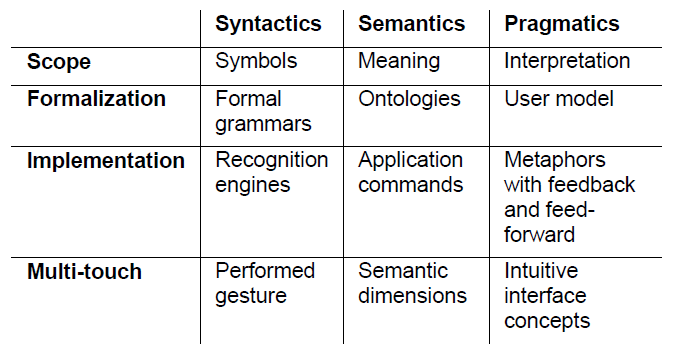
\includegraphics[scale=0.5]{Semiotics}
\end{table}
\end{comment}

% In depth understanding of the different viable gestures or signs that may be used by the user is important to formalize the syntax of gestures. The general term used for gestures is \textit{atomic gestures} \citep{kammer2010towards}. It includes basic shapes like lines, curves, and circles which may still be improved to form more complex gestures. 

% In depth understanding of the different viable gestures or signs that may be used by the user is important to formalize the syntax of gestures. Table \ref{tab:gle} shows the different language elements for GeForMT. The general term used for gestures is \textit{atomic gestures} \citep{kammer2010towards}. It includes basic shapes like lines, curves, and circles which may still be improved to form more complex gestures. 

% Other types of gestures include freeform (MOVE) in which you can assign a command for a specified gesture trail. Another is short contact (POINT, HOLD) which does not require moving the fingers (see Figure \ref{fig:atomicgestures}). One can also specify the direction of a gesture trail like in the case of LINE\_NE.

% Multi-touch also supports simultaneous contacts which can be customized as well using the \textit{composition operators} of GeForMT. Synchronous movements are identified using the asterisk symbol (*) while asynchronous movements are identified using the plus-sign (+). A sequence of atomic gestures may also be defined using a comma delimiter (,). In order to define how two or more atomic gestures relate with one another, prefixes are used. The CROSS prefix is used to indicate overlaps, SYNC for parallel movements, JOIN for converging motion, and SPREAD for separating motion.

% In depth understanding of the different viable gestures or signs that may be used by the user is important to formalize the syntax of gestures and so the research also discussed different possible gestures. Table \ref{tab:gle} shows the different language elements for GeForMT. The general term used for gestures is \textit{atomic gestures} \citep{kammer2010towards}. It includes basic shapes like lines, curves, and circles which may still be improved into more complex gestures. Other types of gesture include freeform (MOVE) in which you can assign a command for a specified gesture trail, and short contact (POINT, HOLD) which does not require movement of fingers (Figure \ref{fig:atomicgestures}). Another type is DEPOINT which refers to the lifting of finger or hands and it can be used as a part of another gesture. Different attributes may be customized depending on the desired gesture. An example would be specifying the direction of a gesture trail (e.g. LINE\_NORTH) and adding focus which is a list of objects used as identifiers. Multi-touch also supports simultaneous contacts which can be customized as well using the \textit{composition operators} of GeForMT. Synchronous movements are identified using the asterisk symbol (*) while asynchronous movements are identified using the plus-sign (+). A sequence of atomic gestures may also be defined using a comma delimiter (,). In order to define how two or more atomic gestures relate with one another, prefixes are used. The CROSS prefix is used to indicate overlaps, SYNC for parallel movements, JOIN for converging motion, and SPREAD for separating motion.

\begin{comment}
\begin{table}[H]
	\centering
    
    \caption{Language elements for GeForMT \citep{kammer2010towards}} \label{tab:gle}
	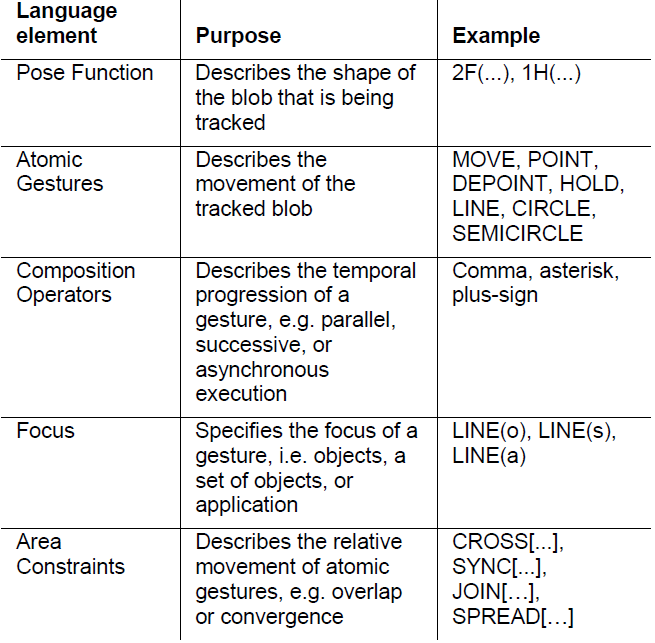
\includegraphics[scale=0.5]{GeForMTLanguageElements}
    
\end{table}

\end{comment}

\begin{figure}[H]
	\centering
	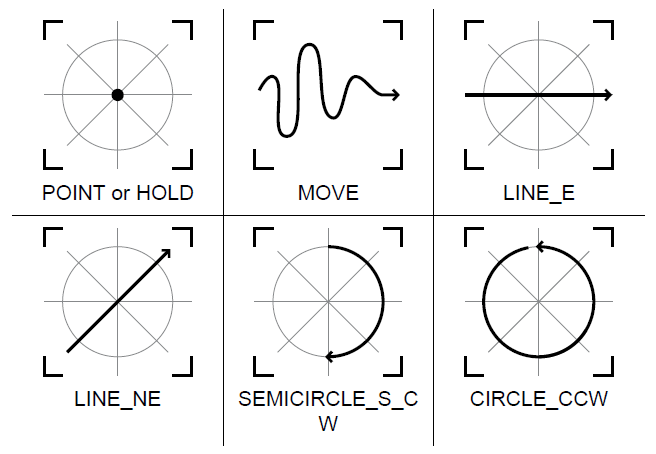
\includegraphics[scale=0.4]{AtomicGestures}
    \caption{Examples of atomic gestures \citep{kammer2010towards}.}
    \label{fig:atomicgestures}
\end{figure}

% The EyesWeb system, developed in the study of \citet{camurri2000eyesweb}, attempts to generate music through human body movement or gestures. The system is equipped with a camera that can detect movements. Its goal is to generate music that is appropriate to the movement it detects \citep{camurri2000eyesweb}. However, since it was an initial study, the system was still limited in terms of movement detection.

The same idea is found in the study of \cite{ip2005cyber}, where a system called the Cyber Composer was developed to make use of hand gestures to create music (see Figure \ref{fig:cybercomposer-media}). The system generated music from blueprints for musical structures. These can be accessed and modified through the use of an external input device called the CyberGlove. This form of input was considered helpful for people without any background in composition. With the help of the CyberGlove, they could create music with only simple hand gestures \citep{ip2005cyber}. However, despite the help provided by the CyberGlove, it was still found to be obtrusive and inaccessible. 

\begin{figure}[H]
	\centering
	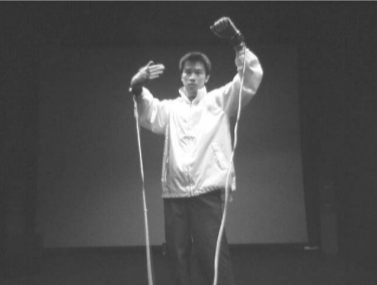
\includegraphics[scale=0.7]{cyberGloveUse}
    \caption{A user operating the CyberGlove \citep{ip2005cyber}.}
    \label{fig:cybercomposer-media}
\end{figure}

In the study of \citet{epps2006a}, the use of gesture interactions as a method of input for tabletop displays was explored. It was found that the index finger was commonly used by the testers when interacting with a large, flat display. Thus, the study recommends to build gesture interactions that mainly revolve around the use of the index finger \citep{epps2006a}.

The aforementioned study of \citet{kikuchi2016music} also used gestures through the use of the Surface Pen. The developed system's mode of interaction involved using the Surface Pen to interact with a Microsoft Surface Pro 3's touchscreen. The simplified interface and intuitive interaction was found to be helpful for inexperienced composers write music.

% The work of \citet{kazi2012vignette} illustrated a similar approach to that of \citet{kikuchi2016music}. 

\citeauthor{kazi2012vignette} developed Vignette, an interactive illustration tool that allows users to manipulate textures through the use of freeform gestures. Although not a musical composition tool, Vignette has similar goals in that it aims to provide an easy-to-use interface that incorporates gestures to augment the illustration process. Texture manipulations such as duplication, synthesis, and fillings can be easily done in Vignette through simple gestures made in the interface \citep{kazi2012vignette}. The overall impressions of users during evaluation were positive, and comments were that it was easy to learn and allowed them to create quick illustrations in only a short time of use.

The later work of \citet{kazi2014draco} builds on Vignette by extending it to allow animations. The new tool, called Draco, is a sketch and animation tool that provides a simplified interface for animation through the use of \textit{kinetic textures}, which is their developed framework for endowing sketched components with motion properties. It allows users to easily create simple animations through intuitive gestures and freeform strokes. Raindrops can be animated by drawing simple curved or linear lines that denote its direction and length of travel.

The earlier study of \citep{mo2005smartcanvas} used cameras to detect gestures. SmartCanvas is a drawing desk system that allows users to create drawings through gestures. This is done with 2 cameras that detect the type of gesture and identify whether or not the user is touching the surface. This resulted in a minimal drawing system without the need for a touchscreen \citep{mo2005smartcanvas}. However, there was one main drawback. Since users would draw on a surface and the drawing would be generated on the computer screen, the user would have to keep switching his/her focus when drawing.

\begin{landscape} % Landscape page
\begin{table} [!htbp]  
\label{tab:rsogi}        
        \captionof{table}{Related Studies on Gesture Interactions}
   \vspace{0.20cm}    
        \begin{tabular}{|p{3cm}|p{4cm}|p{4cm}| p{4cm}| p{5cm} | } %{|l|l|l}
        \hline 
       Authors & Name of Tool & Input/Modality & Types of Gestures & Comments and other findings \\ \hline
       
       \citet{kammer2010towards} & GeForMT & Multi-touch gestures & \makecell[tl]{Tap \\ Point or Hold \\ Linear gestures\\ Circular gestures} & Formalized an approach to create gestures \\ \hline
       
       % \citet{camurri2000eyesweb} & EyesWeb & Cameras & Body movement & Attempts to connect motion to music, but is still limited \\ \hline
       
       \citet{ip2005cyber} & Cyber Composer & CyberGlove & \makecell[tl]{Hand motions \\ Finger bends \\ Finger flexions} & Obtrusive, but allowed composition through hand gestures \\ \hline
       
       \citet{kikuchi2016music} & Music Composition with Recommendation & Microsoft Surface Pro 3 and Surface Pen & Tap gestures & The interface was found to be helpful for inexperienced composers \\ \hline
       
       \citet{epps2006a} & NA & Hand Gestures and Cameras & \makecell[tl]{Single-touch gestures \\ Hand-shape gestures} & The index finger was commonly used for interactions \\ \hline
       
       \citet{kazi2012vignette,kazi2014draco} & Vignette; Draco & Touchscreen device and stylus & \makecell[tl]{Freeform sketches \\ Straight lines \\ Curved lines} & The interface was easy-to-use for beginners and the gestures were intuitive \\ \hline
       
       \citet{mo2005smartcanvas} & SmartCanvas & Touch Gestures and Cameras & Freeform gestures & It was minimal but increased cognitive load due to users having to switch focus when drawing \\ \hline 
       
        \end{tabular}
\end{table}
\end{landscape}

\newpage















               %-- includes LaTeX source file for Chapter 2: Review of Related Literature
                                  %-- your job: **EDIT THIS FILE** to indicate your review of related literature 

%%%%%%%%%%%%%%%%%%%%%%%%%%%%%%%%%%%%%%%%%%%%%%%%%%%%%%%%%%%%%%%%%%%%%%%%%%%%%%%%%%%%%%%%%%%%%%%%%%%%%%
%
%   Filename    : chapter_3.tex 
%
%   Description : This file will contain your Theoretical Framework (Math equations, machine learning algorithms, and the such that will conclude in the realization of the most preferred concepts for constructing the system.
%                 
%%%%%%%%%%%%%%%%%%%%%%%%%%%%%%%%%%%%%%%%%%%%%%%%%%%%%%%%%%%%%%%%%%%%%%%%%%%%%%%%%%%%%%%%%%%%%%%%%%%%%%

\chapter{Theoretical Framework}

This chapter provides a thorough discussion of the different studies and theories behind the three main concepts of this study. The first few sections will tackle research on Human-Computer Interaction. The next set of sections will focus on User Experience Evaluation methods, and finally, Musical Composition and Metacreation. 

\section{Human-Computer Interaction}

	The study of Human-Computer Interaction (HCI) is about how technology can make an impact to human life \citep{dix2009human}. Its birth can be traced back to the studies of \citet{shackel1959ergonomics} and \citet{engelbart1962augmenting}. Both studies explored the approach of developing systems or interfaces for the benefit of the human intellect. This research stemmed from the increasing complexity of human tasks, and the need for technology to augment the capabilities of humans when performing these tasks \citep{engelbart1962augmenting}.
    
    HCI is multi-disciplinary, borrowing principles and theories from psychology, sociology, and computer science \citep{dix2009human, sinha2010human}. In HCI, one must learn to understand the users, which can be done through user observation or interviews, to develop systems and interfaces that would fit their backgrounds and needs \citep{fischer2001user}.
    
	One of the core topics in HCI is the issue of usability \citep{frokjaer2000measuring, dix2009human}. Usability tackles questions about effectiveness, efficiency, and satisfaction. Effectiveness asks if users can achieve their goals or perform their tasks properly and correctly when using the system \citep{frokjaer2000measuring}. Efficiency talks about whether users can perform the said goals with minimum use of resources or effort \citep{frokjaer2000measuring}. Finally, satisfaction is about finding out if users enjoy using the system or feel comfortable using it \citep{frokjaer2000measuring}. These usability issues can be achieved through the proper use of design principles (discussed in Section \ref{sec:designprinciples}).

    The growth of technological study and the emergence of new technological platforms brought with it new subfields under Human-Computer Interaction such as interaction design, user interface software technology, and user experience.
    
	\subsection{Interaction Design}
    
    Interaction functions as an essential factor to society's progress \citep{rogers2011interaction}. Humans interact with other humans or objects on a daily basis. These objects could be mobile phones, laptops, ATMs, and more. But not all of these have good usability or interaction. In that case, the interaction of these objects might not have been designed with the user in mind \citep{rogers2011interaction}. Even though these objects may be considered usable, they might not provide the best user experience when being used. 
    
    The goal of interaction design is to lessen these bad experiences when using objects, or in this case, technology \citep{shedroff1999information,rogers2011interaction}. User satisfaction is imperative to interaction design. It is about designing interactions that would not only benefit users, but would also reduce cognitive load and make the experience enjoyable or pleasurable \citep{tidwell2010designing}. 
    
    The continued study of interaction design allowed researchers and designers to identify a set of design principles. These principles serve as guidelines to designing good interactions and interfaces \citep{rogers2011interaction}. 

	\subsubsection{Design Principles}
    \label{sec:designprinciples}
    
    	What most developers or software development companies forget is that it is not always about how aesthetically pleasing the product is, rather, it is about how functional and easy it is for users of varying experience to understand how to use it \citep{blair2008user}. The overall system design should incorporate both functionality and visual appeal to provide value to its users.
        
        According to \citet{blair2008user}, the goal of the software should be decided and set at the start so that the interface is designed to support that goal. The design should make it obvious what the goal is all about. However, this should not make the design any less aesthetically pleasing. The designer should keep in mind what the software aims to do as well as making it pleasing for users to view and use. 
        
        Developers and designers should work together to form the design and user interface of the system. According to \citet{galitz2007essential}, the interface is the most important part of the system because it is what the users could see and interact with all the time. A testament to this importance is the finding that good design could help users become more productive and reduce cognitive load by up to 40\% \citep{galitz2007essential}. 
        
        Similarly, it was found in the study of \citep{cope1995cost} that redesigning just one web page to follow good design standards allowed a company to cut costs by \$20,000. This redesigned web page increased user productivity and reduced user error and training time. 
        
        \citet{mandelbaum2014design} notes four key principles to consider when designing products and interfaces (see Table \ref{tab:key-design-principles}):
        
        \begin{longtable}{|p{2cm}|p{11.6cm}|} 
        \caption{Key Design Principles} \label{tab:key-design-principles} \\
        \hline
        
        	Design Principle & Description \\ \hline
            
            Axis & The Axis, is an imaginary line that arranges, and aligns elements \citep{mandelbaum2014design}. It is considered as the most basic of the principles, but is equally important. When objects in an interface fall in or follow one axis, the design would give the impression of order. The axis allows movement in a straight line that the user's eyes can follow \citep{mandelbaum2014design}. The axis directs users towards something in the design. \\ \hline
        
        	Symmetry & The second principle, Symmetry, works together with the axis to promote balance \citep{mandelbaum2014design}. Symmetry enables balance between both sides of the axis, aligning and making both sides of an interface similar. Having symmetry gives users the feeling of harmony, and even the slightest difference in alignment or order can throw of the balance of a design and give a feeling of discomfort \citep{mandelbaum2014design}. \\ \hline
        
        	Hierarchy & Hierarchy is about showing the importance of certain elements in a design \citep{mandelbaum2014design}. One example of this is making one article in a news feed larger than the rest. The larger article would catch the users attention first and give the impression that it is more urgent or important compared to others. Other ways to show hierarchy could be through its placing or its shape. \\ \hline
        
        	Rhythm & Lastly, Rhythm, denotes patterns in the design. Having rhythm in the design allows users to find patterns and better recognize and know where to look for particular information \citep{mandelbaum2014design}. This can be seen in a Twitter feed where a list of tweets would look the same, helping users where to find the like button, or the user's twitter handle, etc. \\ \hline
           
        \end{longtable}
        
        Although they are not solid rules, these principles can be considered as building blocks that can be used to build an interface. The design is considered as the most important element of the system because it is what user can see and interact with \citep{galitz2007essential}.. Thus, careful consideration should be put in an application's overall design.
        \begin{comment}
        
        
        \begin{itemize}
        	\item Axis
            \item Symmetry
            \item Hierarchy
            \item Rhythm
\end{itemize}
        
        The axis, is an imaginary line that arranges, and aligns elements \citep{mandelbaum2014design}. It is considered as the most basic of the principles, but is equally important. When objects in an interface fall in or follow one axis, the design would give the impression of order. Additionally, the axis allows movement since it is a straight line that the user's eyes can follow \citep{mandelbaum2014design}. This movement can be used to direct users towards something in the design.
        
        The second principle, symmetry, works together with the axis to promote balance \citep{mandelbaum2014design}. Symmetry means balancing both sides of the axis, meaning both sides of an interface should be similar, and aligned. Having symmetry gives users the feeling of harmony, and even the slightest difference in alignment or order can throw of the balance of a design and give a feeling of discomfort \citep{mandelbaum2014design}.
        
        Hierarchy is about showing the importance of certain elements in a design \citep{mandelbaum2014design}. One example of this is making one article in a news feed larger than the rest. The larger article would catch the users attention first and give the impression that it is more urgent or important compared to others. Other ways to show hierarchy could be through its placing or its shape.
        
        Lastly, rhythm, denotes patterns in the design. Having rhythm in the design allows users to find patterns and better recognize and know where to look for particular information \citep{mandelbaum2014design}. This can be seen in a Twitter feed where a list of tweets would look the same, helping users where to find the like button, or the user's twitter handle, etc. 
        
        Although they are not solid rules, these principles can be considered as building blocks that can be used to build an interface. Again, careful consideration should be put in the design because it is considered as the most important element of the system because it is what the users can see and interact with \citep{galitz2007essential}.
        
        \end{comment}
        
	\subsubsection{Information Design}
    
		Communication is an essential aspect of the everyday lives of people. In businesses, it is important that they are able to communicate and get the point across to their clients and consumers. To do this, information must be designed in a way that can easily and efficiently be used and understood by people. This is where the art of information design comes in \citep{horn1999information}.
        
        An integral part of interaction design, information design involves analysis and understanding of not only the content of the message or information, but how it will be presented as well \citep{pettersson2002information}. It is about how to clearly communicate or send across information which is a key aspect in designing a good interaction \citep{shedroff1999information}.
        
        It is with proper organization that good information design is achieved, which can also lead to good interaction design \citep{shedroff1999information}. Information can be organized in several ways such as: alphabet, location, similarities, and more. Organizing these in such a way allows users to better understand and connect the individual piece of information \citep{shedroff1999information}. Additionally, \citet{blair2008user} advises the use of visualizations such as charts or graphs when presenting large information in order to make it easier for people to digest the information. 
        
        Even though information design is its own discipline, it should still follow the common design principles so that the information can be presented neatly and effectively \citep{shedroff1999information}. The information, or the way it is presented, is still a part of the overall design of the system so similar to designing an interface, it is good practice that designers keep in mind the goal of the system when trying to formulate how the information will be presented. 
        
        Going back to the hierarchy principle, the most important information should be presented in a way that would easily grab a user's attention like making it larger than the others or placing it at a position that can easily be seen \citep{mandelbaum2014design}. This just goes to show that the design principles mentioned above encompass all kinds of design, from visual design to information design.

	\subsubsection{Input and Interaction}
    	
        Without humans, there would be no technology \citep{commoner2014closing}. Despite machines being more computationally powerful and efficient, there is still a need for human input. Because of the emergence of several machines for daily use, different input methods have been developed. 
        
        For computers, there was the mouse, keyboard, tablet, and trackball, with the mouse and keyboard being the most popular \citep{engelbart1968a, mackenzie1991a}. With the rise in popularity of mobile phones, users can now interact with touch screens through gesture interactions \citep{chen2014agraph}. As such, these methods of input will be further discussed in the next few chapters.
    
    % add opener

		\paragraph{Traditional Computer Input}
        
      	During the advent of the computer becoming a consumer product, the keyboard and mouse were present to accompany the Windows, Icons, Menus, and Pointing Devices (WIMP) interaction style \citep{porta2007human}. The keyboard and mouse were also innovations during their time. Both were used to test how new kinds of interaction between a human and computer could augment the overall output of a computer user \citep{engelbart1968a}. 
        
        %As such, this section will discuss how each of these input devices have affected or furthered the progress of Human-Computer Interaction during their time.

Keyboards were mainly used to type commands into a computer device to fulfill a task the user would like to do \citep{karat1986a}. In the earlier times, keyboards were used alongside a command line interface, which made up most of the interaction during the time where graphical user interfaces were yet to be known \citep{galitz2007essential}. The keyboard is usually accompanied by a mouse where they are used in conjunction to perform tasks with computers \citep{engelbart1968a}. There have been events to also increase the comfort of using the keyboard to create less strain on the wrists or arms of the user \citep{grant1994computer}.  

            %Keyboards were mainly used to type commands into a computer device to fulfill a task the user would like to do \citep{karat1986a}. In the earlier times, keyboards were used alongside a command line interface, which made up most of the interaction during the time where graphical user interfaces were yet to be known \citep{galitz2007essential}. The keyboard's keys can also be used to navigate menus that are designed to be traversable through specific keys on the keyboard. The keyboard is usually found in a workstation accompanied by a mouse or pointer for both their features to be used in conjunction with a computer in hopes to fulfill tasks quicker \citep{engelbart1968a}. There have been events to also increase the comfortability of using the keyboard to create less strain on the wrists or arms of the user \citep{grant1994computer}.  

The mouse is a commonly used tool for navigating a 2D space in a computer screen \citep{engelbart1968a}. A standard mouse has three (3) buttons that can be used to select or perform additional tasks on the computer. Other devices were also built to navigate a 2D space, but the mouse was found to be the best performer among these devices \citep{karat1986a}

            % The mouse was found to be the faster way compared to other devices like light pens or joysticks when navigating a 2D space in the screen of a computer \citep{engelbart1968a}. A standard mouse can have 3 buttons mainly to be used when a user is ready to select whatever is pointed by the pointer on the computer screen. There are also devices that can be used to navigate the 2D space but it was found that the mouse performed the best during tests \citep{karat1986a}.

		% Add more
        
        	These traditional methods of input are commonly used in musical composition applications like Finale or Sibelius. In these applications, users usually input notes or modify the composition through a series of mouse clicks, while the more experienced users perform keyboard shortcuts \citep{knoder2017sibelius,knoder2017finale}. These methods can be efficient and easy, however the main drawback of these is that the keyboard and mouse are not easily portable, and are definitely not natural \citep{norman2010natural}.

		Touch-based interfaces were introduced at a later time to complement touchscreen devices and were meant to take advantage of the natural way humans interact. This was another step into finding out ways to improve the interaction between a human and a computer \citep{travis2014comparative}. 
       
        
		\paragraph{Gestural Interaction}

The goal of Human-Computer Interaction is to allow humans to interact with machines or computers naturally and seamlessly \citep{hasan2012human}. There is an increase in the use of gestures as a method of interaction in hand-held touch devices like tablets and smart phones and this is mainly attributed to gestures being considered as an an easy and natural method of interaction between humans and computers, compared to the use of a mouse or a stylus \citep{kurtenbach1996gestures, pavlovic1997visual, hasan2012human}. 

As most gestures found in gesture interaction systems are based on semiotics, \citep{muntigl2004modelling,radford2009introduction, kammer2010towards}, it is important to understand how gestures play a part in communication.

The work of \citet{wesp2001gestures} supports the idea that gestures help maintain spatial imagery. The use of gestures in communication helps in word retention because it builds up an idea through its perceivable signs \citep{krauss1998why}. This also applies to touch gestures since they build up perceivable actions that denote specific functions which make them an intuitive and natural way of interaction \citep{rautaray2015vision}.

In the study presented by \citet{roth2001gestures}, a gesture can be defined using four characteristics. The first characteristic of a gesture is that it moves from a resting position to a non-resting position and then back to a resting position. The second, \textit{stroke}, defines the peak structure of the gesture where it denotes the function of the gesture movement. The third, \textit{preparation} and \textit{recovery} phase, is when the stroke goes back to its resting position. The fourth characteristic is that it is symmetrical.

Recent studies on gestures led to its taxonomy wherein they are are classified based on their functions or how they were modeled \citep{roth2001gestures}. There are four classifications of gestures according to \citet{mcneill2007hand} (see Table \ref{tab:classifications-of-gestures}):

\begin{longtable}{|p{3cm}|p{10.6cm}|}
\caption{Classifications of Gestures} \label{tab:classifications-of-gestures} \\
\hline

Gesture & Description \\ \hline

\textit{Beats} or \textit{Batons} & These are gestures that do not express opinions. They are simple gestures which include slight movement of hands such as tapping or flicking that express responsiveness. \\ \hline

\textit{Deictic} gestures & These gestures attribute a contextual meaning such as pointing or extending of arms or hands. They are commonly used in referring to people or referring to locations. \\ \hline

\textit{Iconic} gestures & Iconic gestures use hand movements which relate to concrete objects.  \\ \hline

\textit{Metaphorical gestures} & These are movements that relate to a certain concept and makes a visual reference to it. An example would be a professor telling the class about the destruction of the world while closing his hands slowly. \\ \hline

\end{longtable}

% The first type, \textit{beats} or \textit{batons}, are gestures that do not express opinions. They are simple gestures which include slight movement of hands such as tapping or flicking that express responsiveness. The second type of gesture, \textit{deictic} gestures, are gestures that attribute a contextual meaning such as pointing or extending of arms or hands. They are commonly used in referring to people or referring to locations. The third type, \textit{iconic} gestures, are gestures that use hand movements which relate to concrete objects. The fourth type, metaphorical gestures, are movements that relate to a certain concept and makes a visual reference to it. An example would be a professor telling the class about the destruction of the world while he is closing his hands slowly.
        
			\subparagraph{Touch Gestures}        

Touch gestures have been widely used in recent years because of its intuitive and convenient nature \citep{chen2014agraph}. Some commonly used gestures in touch screen devices are pinching, scrolling, and tapping. There are three different types of touch-based interactions. The first one, raw ink, records the freehand drawing of the user. Sketching applications such as Paint is an example that uses this type of touch interaction. The second one, direct manipulation, is used in manipulating the user interface and gives real-time feedback to the user such as zooming and scrolling. The third one, indirect command, treats gestural input as a shortcut function in an application such as undo, redo, copy, and paste \citep{chen2014agraph}. In this study, direct manipulation will be used as the primary type of touch interaction for metacreation and other functionalities. 
            
The work of \citet{chen2014agraph} presents a way to recognize multi-touch gestures and assign specific functions for each with the use of graph modeling. In order to do so, it is important first to discern the difference between direct manipulation and indirect command. Direct manipulation calculates the position between fingers and it gives continuous feedback to the user while performing a gesture. For example, the act of pinching to zoom out a text document requires the system to continuously change the view in sync with the pinching motion. Indirect command, on the other hand, is concerned with the motion's shape and trajectory right after when the user performed a gesture. It captures the shape of motion after it has been performed and executes the assigned function. 

There are three types of information that needs to be considered when modeling a multi-touch gesture \citep{chen2014agraph}. The first one, spatial, stores the position of each gesture trail relative to each other. The second one, temporal, stores the order of trails and their corresponding duration. The third one, shape information, stores the shape of each trail which allows the system to distinguish the difference between a straight line swipe from a curve swipe.

Each gesture trail can be represented by three vertices in a graph \citep{chen2014agraph}. The first vertex, ($V_b$), represents the begin vertex. The second vertex, ($V_s$), represents the stroke vertex, and the third vertex, ($V_e$), represents the end vertex. Temporal and spatial information are represented using the following edges: $E_s$(x, y), $E_{st}$(x, y, t), and $A_{st}$(x, y, t), wherein subscripts s and st indicate whether an edge represents only spatial, or both spatial and temporal, respectively. Consider the following example in Figure \ref{fig:spatial-temporal-graph}:

\begin{figure}[H]
	\centering
	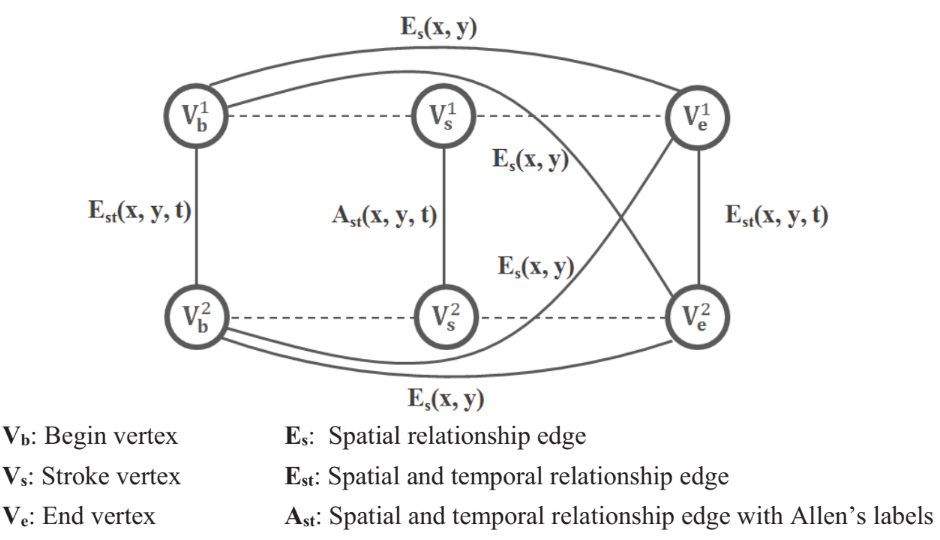
\includegraphics[scale=0.5]{SpatialTemporalGraph}
    \caption{An example of a two strokes gesture graph \citep{chen2014agraph}.}
    \label{fig:spatial-temporal-graph}
\end{figure}

In order to complete the information of the edges in Figure \ref{fig:spatial-temporal-graph}, Allen's relations that use discrete labels of time will be used as shown in Figure \ref{fig:allen-relations}.

\begin{figure}[H]
	\centering
	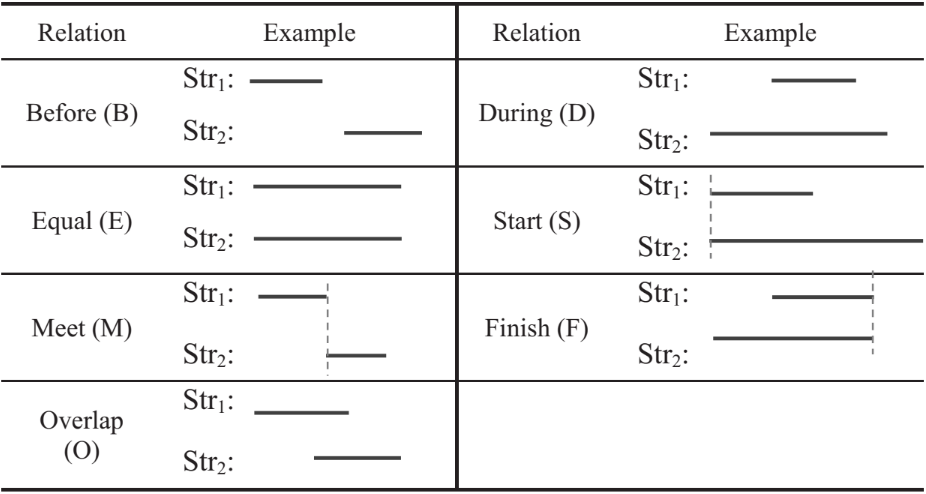
\includegraphics[scale=0.5]{AllenRelations}
    \caption{Examples of Allen's relations \citep{allen1983maintaining, chen2014agraph}.}
    \label{fig:allen-relations}
\end{figure}

In general, labeling the edges results in two possible cases:

\begin{enumerate}
\item \textit{Edges between stroke vertices ($A_{st}$)}: This represents the measurement and relationship of strokes with regards to time, x-axis, and y-axis. 
\item \textit{Edges between extremity vertices ($E_s$ and $E_{st}$)}: This represents the touching and lifting of fingers in a touch screen and so it only encompasses \textit{Equal} property for the time \textit{(E\_T)}, x-axis position \textit{(E\_X)}, and y-axis position \textit{(E\_Y)} in defining the edges between vertices.
\end{enumerate}


Shown in Figure \ref{fig:flick} is a flick gesture with its corresponding spatial relation and time duration. According to the relations of \citet{allen1983maintaining}, the flick gesture has an \textit{Equal\_X (E\_X)} and \textit{Before\_Y (B\_Y)} labels which denote that the x-coordinates of both strokes are equal and the y-coordinate of the first stroke is above (Before) the y-coordinate of the second stroke. The time duration is labeled as \textit{Equal\_T (E\_T)} to denote that the strokes were simultaneously performed. This results into edge \textit{$A_{st}$} having an equation: $A_{st}$(x, y, t) = \{E\_X, B\_Y, E\_T\}

\begin{figure}[H]
	\centering
	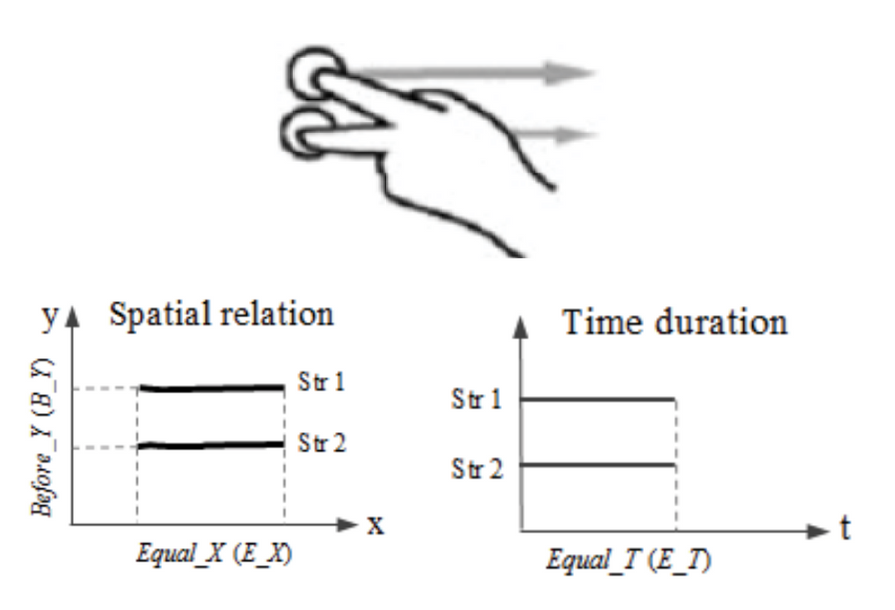
\includegraphics[scale=0.4]{flick_gesture}
    \caption{Flick gesture \citep{chen2014agraph}.}
    \label{fig:flick}
\end{figure}

\begin{comment}
\begin{figure}[H]
	\centering
	\includegraphics[scale=0.6]{Flick}
    \caption{Flick gesture \citep{chen2014agraph}}
    \label{fig:flick}
\end{figure}

\begin{figure}[H]
\centering
\begin{minipage}{.4\textwidth}
	\centering
	\includegraphics[width=.7\linewidth]{SpatialRelation}
    \caption{}
    \label{fig:spatial-relation}
\end{minipage}
\begin{minipage}{.4\textwidth}
	\centering
	\includegraphics[width=.7\linewidth]{TimeDuration}
    \caption{}
    \label{fig:time-duration}
\end{minipage}
\end{figure}
\end{comment}
In the graph of the flick gesture, the label $E_{st}$=\{E\_X, E\_T\} at the left and right side denote that the x-coordinates of both strokes are in the same region and they were performed at the same time. The label $E_{st}$=\{E\_Y\} on the top and bottom of the graph denote that both strokes were performed in the same region of the y-coordinate.

\begin{figure}[H]
	\centering
	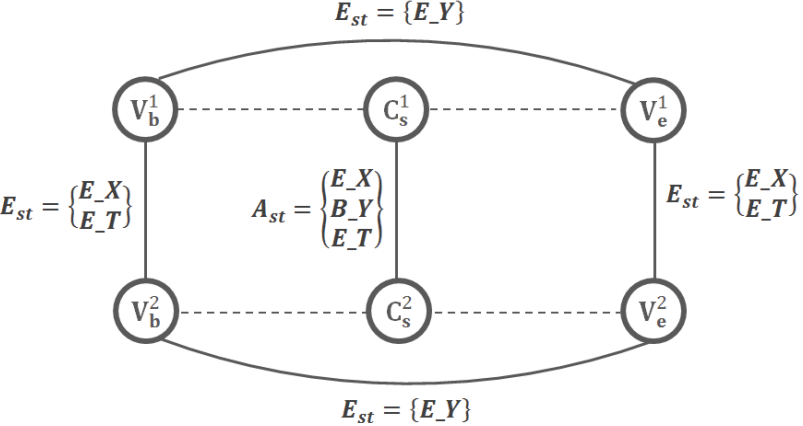
\includegraphics[scale=0.5]{FlickGraph}
    \caption{Flick graph \citep{chen2014agraph}.}
    \label{fig:flick-graph}
\end{figure}

In the application's selected platform, iOS, gestures are recognized through the \texttt{UIGestureRecognizer} class, implemented in the Swift programming language. This class is the one that detects gestures and passes them to other related objects that would act on that gesture. An important thing to note is that it does not perform anything related to the gestures, it only passes them. This was done in order to decouple the logic for recognizing the gesture and acting on it \citep{apple2017ui}.

By default, the \texttt{UIGestureRecognizer} class allows the detection of common gestures like taps, holds, pinchs, and more through its subclasses \citep{apple2017ui}. It communicates with \texttt{UIGestureRecognizerDelegate} classes to better control gestures in applications. The way gestures work in iOS is that the window or view reads the gestures and checks if any \texttt{UIGestureRecognizer} object recognizes the gesture performed. If one does, it would then pass control to that object \citep{apple2017ui}. 

	\subsection{User Interface Software Technology} 
    \label{sec:uist}
		
        With the large, yet still growing number of applications and software available in the market today, it is becoming increasingly hard for developers to make their application stand out. One important factor that decides an application's fate in the market is design \citep{deka2016datadriven}.

		Application design is a process \citep{curtis1988field,humphrey1995discipline} that takes time and effort not only from designers, but from developers and researchers as well. They must identify how best to design the interface in a way that users would find intuitive and natural. This process involves research on the users' needs and behaviors and user experience validation through testing and heuristics \citep{deka2016datadriven}. 
        
        Jakob Nielsen presents set of usability heuristics to follow for interface design \citep{nielsen1990heuristic, nielsen1994usability, nielsen2013usability}:
        \begin{itemize}
        	\item Visibility of system status
            \item Match between system and the real world
            \item User control and freedom
            \item Consistency and standards
            \item Error prevention
            \item Recognition rather than recall
            \item Flexibility and efficiency of use
            \item Aesthetic and minimalist design
            \item Help users recognize, diagnose, and recover from errors
            \item Help and documentation
		\end{itemize}
		
        \textit{Visibility of system status} denotes that users should always be informed about what's currently happening in the system. For example, the application is loading, then it should show that it is loading and not just a blank screen so the user won't think that the application froze.
        
        \textit{Match between system and the real world} means that systems should follow what is natural to the user. It should speak in the user's same language, using words and icons that the user can understand. 
        
        The \textit{user control and freedom} heuristic simply means that the user should be able to easily undo or redo their state in case of a mistake. 
        
        \textit{Consistency and standards} denotes that there should be consistency in the words used and the design. The system should not make the user think whether two buttons with the same name do different things.
        
        \textit{Error prevention} is important so that there will not be a need for error recovery. It is better to prevent users from committing errors rather than forcing them to recover from an error they made.
        
        \textit{Recognition rather than recall} should be kept in minding when designing a user interface to help reduce the cognitive load of users when using the system. Objects or icons should be clearly visible and easily retrievable to users.
        
        \textit{Flexibility and efficiency of use} means that the system should be more flexible to allow experienced users to speed up interaction or use shortcuts. 
        
        Systems should have \textit{aesthetic and minimalist design} that only shows relevant information to the user. This is so that the screen clean and reduce the cognitive load of the user. 
        
        Systems should \textit{help users recognize, diagnose, and recover from errors} through information that could easily be read and understood.
        
        \textit{Help and documentation} should also be included in the case that users would want to understand how to use the system better.
    

\section{User Experience Evaluation}

		User experience plays a key role in software development as it can drastically increase a product's return of investment \citep{bellamy2011deploying}. Usability allows the discovery of problems sooner which may save a lot of budget costs and may improve sales. Producing applications that are usable is often difficult to pull off in actual practice because of its iterative process which uses human observation and analysis. This implies that there are biases in terms of testing and analysis \citep{bellamy2011deploying}. Over the years, multiple solutions for user experience evaluation have been proposed.

	\subsection{Quantitative Evaluation}
    
    	\subsubsection{KLM-GOMS}
        	
            One example of a quantitative method for analyzing the usability of an application is by using \textit{cognitive modeling}, an analytic technique that measures the motor operations performed by the user with regards to the brain \citep{sauro2009estimating}. An example of this is measuring how fast a user can navigate an interface or interact with it. 
            
            The most commonly used cognitive modeling technique is GOMS, which stands for Goals, Operators, Methods, and Selection Rules. GOMS is a set of models for analyzing human-computer interaction and for removing user actions which are deemed useless or unnecessary \citep{card1983the}.
            
            One such example of a GOMS technique is the Keystroke Level Modeling (KLM) technique \citep{sauro2011measuring}. It is commonly used by practitioners due to its simplicity. The KLM technique is used to estimate user actions such as pointing, clicking, typing, and thinking \citep{sauro2009estimating}. The technique simply counts the number of operations it would take a user to achieve a certain goal or navigate a system. From there, ideas can be gained from where the users experience pain points when using the system. 
       
    	\subsubsection{Fitts' Law}
        
    		Another, and more descriptive method of analyzing usability is the Fitts' Law. Fitts' law is a predictive model for human movement that takes into account the distance from the target and the time it took the user to navigate to that target \citep{mackenzie1992fitts}.
            
            Fitts' Law was conceived from information theory, specifically that of Shannon's Theorem 17 (Equation \ref{eq:shannon}), which denotes the information capacity (\begin{math}C\end{math}), or the amount of information that can be sent, using a signal power (\begin{math}S\end{math}) within a specified bandwidth (\begin{math}B\end{math}), while affected by noise (\begin{math}N\end{math}) \citep{mackenzie1992fitts}.
            
            \begin{equation}
            	\label{eq:shannon}
            	C = Blog_2 \frac{S + N}{N}
            \end{equation}
    
    		Although there was no direct mathematical relation of Fitts' Law to that of Shannon's Theorem, Fitts got the idea from the theorem of how information is processed through human channels when performing tasks \citep{mackenzie1992fitts}. He derived some of the elements of information theory to form what is now called Fitts' Law (Equation \ref{eq:fitts}), where the index of performance (\textit{IP}) can be derived by dividing the specified task's index of difficulty (\textit{ID} by the movement time (\textit{MT}) it took to perform the task. 
            
            \begin{equation}
            	\label{eq:fitts}
            	IP = \frac{ID}{MT}
            \end{equation}
            
            From this, Fitts Law can be used in domains like physical movement, or movement on a digital screen. Using Fitts Law, pain points can be identified, and interface elements that affect a user's effectiveness when performing tasks can be found \citep{mackenzie1992fitts}. 
            
            Fitts Law will be heavily used in the study to help the researchers identify these pain points in the design. It will provide a numeric measure on the effectiveness of a user interface, making it easier for the researchers to document and compare results between previous versions of the interface. The measurement of Fitts Law can be made easier through CogTool (to be discussed in Section \ref{sec:cogtool}), which will also be used in this study. 
            
    	\subsubsection{CogTool}
        \label{sec:cogtool}
        
        % User experience plays a key role in software development as it can drastically increase a product's return of investment \citep{bellamy2011deploying}. Usability allows the discovery of problems sooner which may save a lot of budget costs and may improve sales. Producing applications that are usable is often difficult to pull off in actual practice because of its iterative process which uses human observation and analysis. This implies that there are biases in terms of testing and analysis. Over the years, a solution was proposed.
        
        
        Although useful for quantitatively understanding the user experience of an application, both KLM and Fitts' Law require that the users being tested are observed in order to calculate the time and make estimates for both models. This poses a problem because it requires manual work and is repeated multiple times depending on the number of tests required. Having to manually make estimates for KLM and Fitts' Law can be tedious and prone to error \citep{sauro2009estimating}. However, IBM's solution for this problem is the implementation of an iterative and quantifiable method of testing and analyzing a product's usability through the software, \textit{CogTool}. 
         
         CogTool is similar to other prototyping tools like InVision, but is more powerful for quantitative evaluation. Once an application's interface has been set in CogTool, with the simple click of a button a cognitive model for evaluation will be generated. CogTool eliminates the need to manually calculate KLM or Fitts Law, making it easier to quantitatively evaluate a user interface \citep{bellamy2011deploying}. 
         
		It uses \textit{storyboards} that demonstrate the different tasks of a user \citep{bellamy2011deploying}. These storyboards serve as the user interface of the system that is being tested. Inside these storyboards are \textit{frames} that serve as the different states of the UI. Each frame may have \textit{widgets} which can be used by the user to interact with. The assigned action for each widget is called \textit{transition}. A sample storyboard is shown in Figure \ref{fig:cogtool}. The rectangles inside the storyboard are the frames. The orange area inside the frame is the widget. The arrow between the frames is the transition.
        
       % Having to manually make estimates for KLM and Fitts' Law can be tedious and prone to error \citep{sauro2009estimating}. However, IBM's solution for this problem is the implementation of an iterative and quantifiable method of testing and analyzing a product's usability through the software, \textit{CogTool}. CogTool is similar to a prototyping tool like InVision, but it is more powerful as it also analyzes the behavior of a user while interacting with the designed prototype. It uses \textit{storyboards} that demonstrate the different tasks of a user \citep{bellamy2011deploying}. These storyboards serve as the user interface of the system that is being tested. Inside these storyboards are \textit{frames} that serve as the different states of the UI. Each frame may have \textit{widgets} which can be used by the user to interact with. The assigned action for each widget is called \textit{transition}. A sample storyboard is shown in Figure \ref{fig:cogtool}. The rectangles inside the storyboard are the frames. The orange area inside the frame is the widget. The arrow between the frames is the transition.
        
\begin{figure}[H]
	\centering
	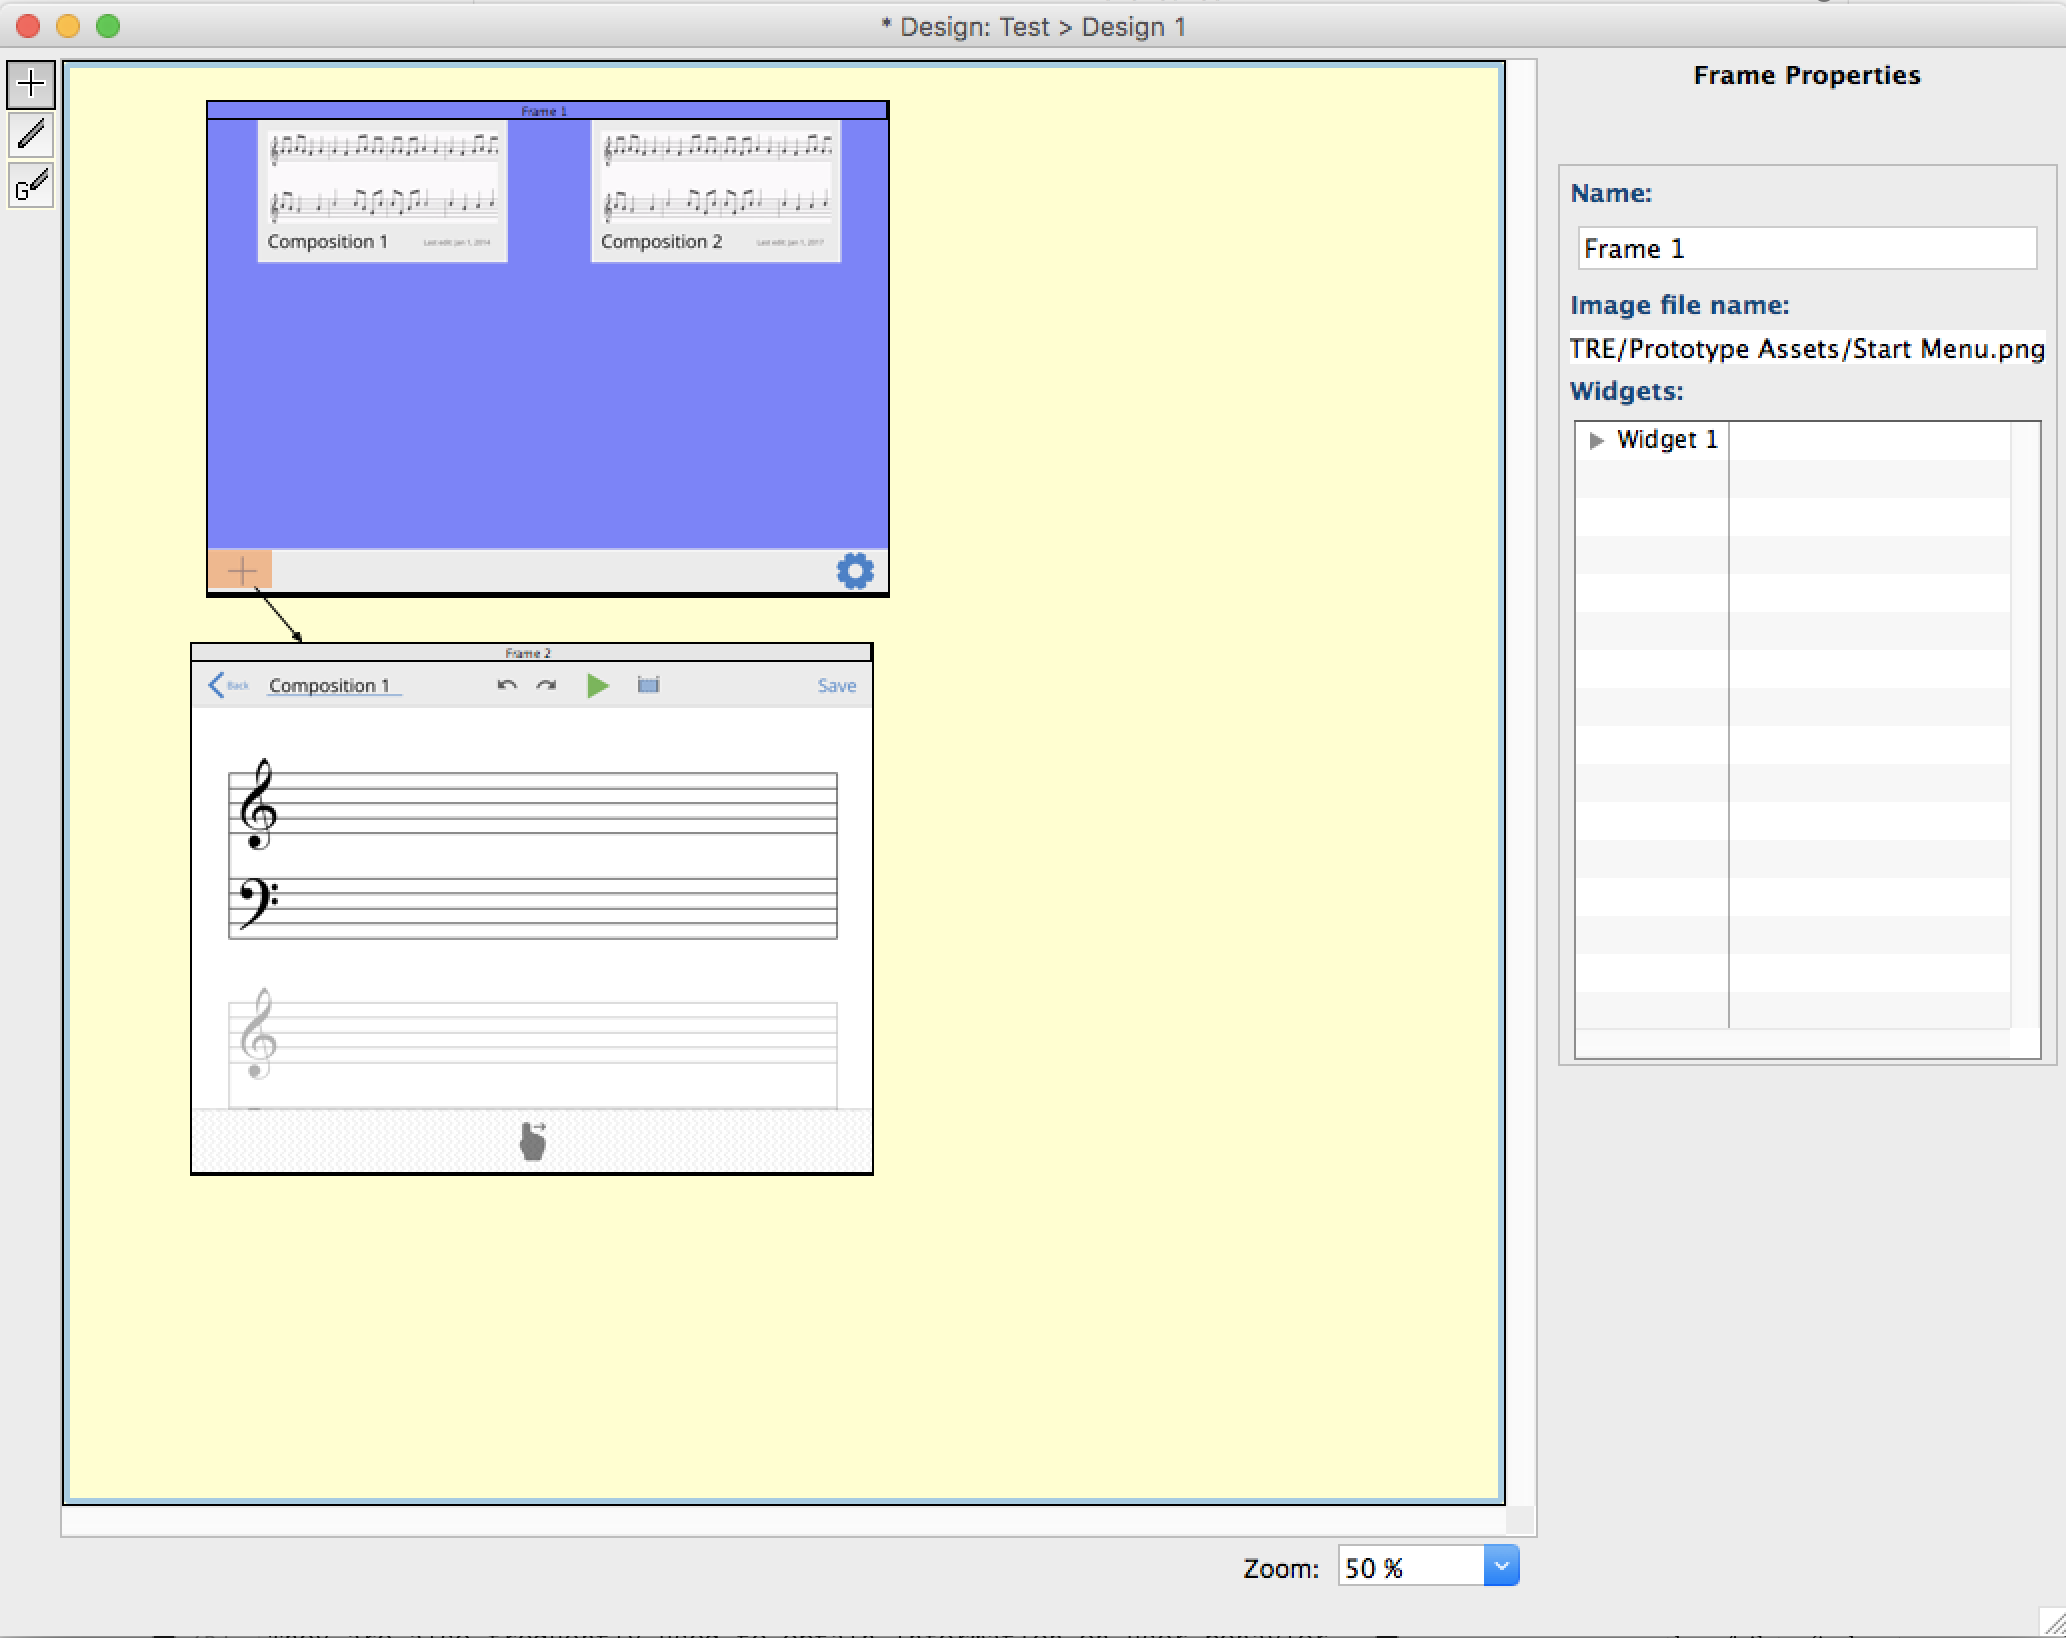
\includegraphics[scale=0.4]{CogToolMockup}
    \caption{CogTool storyboard of application mockup.}
    \label{fig:cogtool}
\end{figure}
        
        Once a storyboard has been setup completely, a starting frame must be chosen for the system to start with (see Figure \ref{fig:start-frame}).
        
\begin{figure}[H]
	\centering
	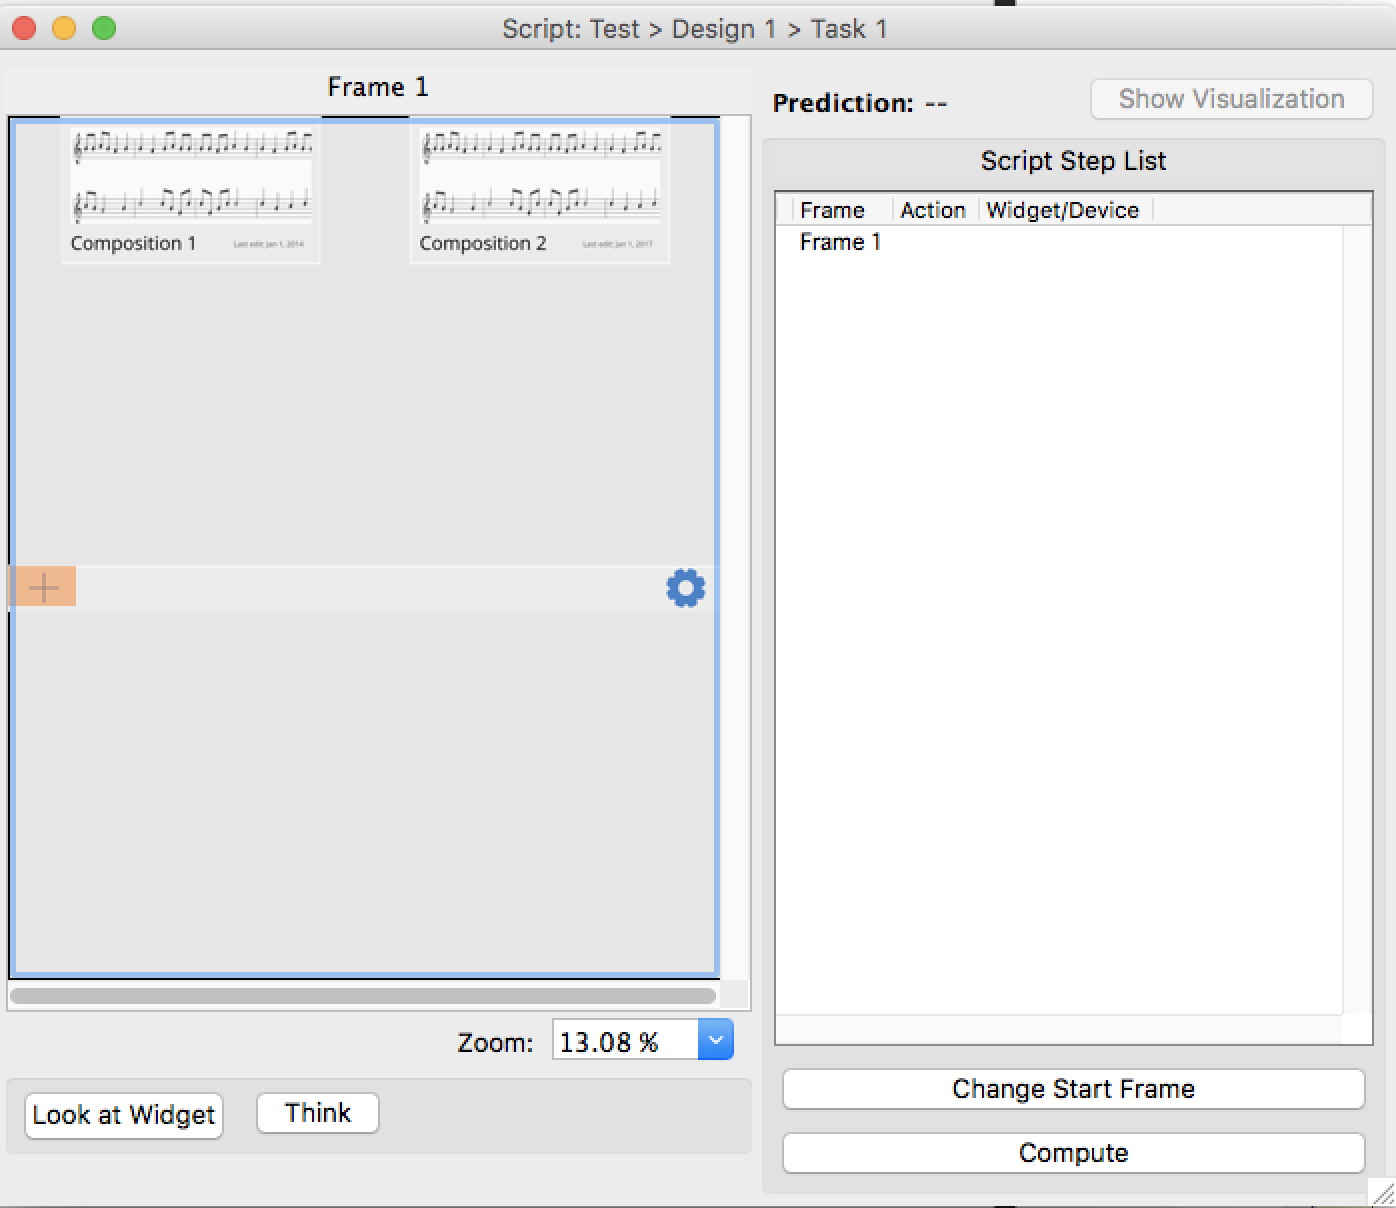
\includegraphics[scale=0.5]{StartFrame}
    \caption{Choosing a start frame for a storyboard.}
    \label{fig:start-frame}
\end{figure}
        
        CogTool has the ability to run an automated user that would go through the whole storyboard. The steps that the automated user takes will also be shown in the script step list (see Figure \ref{fig:script-step}). The list allows designers and analysts to easily identify what the user is doing and how long it takes the user to do it.
        
        % CogTool records all the actions performed by the user and it also records the idle times when the user is not doing any action. Figure \ref{fig:script-step} shows the script step list of CogTool where all the actions are shown while the user is interacting with the storyboard.
        
\begin{figure}[H]
	\centering
	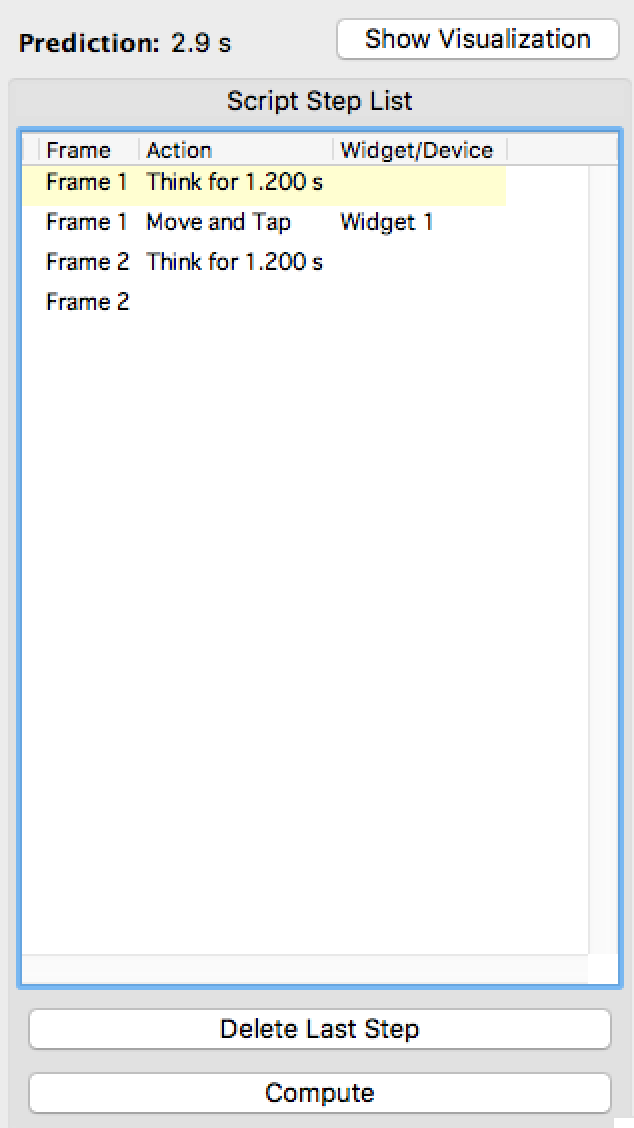
\includegraphics[scale=0.6]{ScriptSteps}
    \caption{Script step list of CogTool.}
    \label{fig:script-step}
\end{figure}  

When the user clicks on the compute button, CogTool computes for the estimate of the quantitative time of execution and visualization of timeline. The visualization shows the different tasks of the cognitive model on how it was able to derive the estimate (see Figure \ref{fig:cogtool-visual}).

\begin{figure}[H]
	\centering
	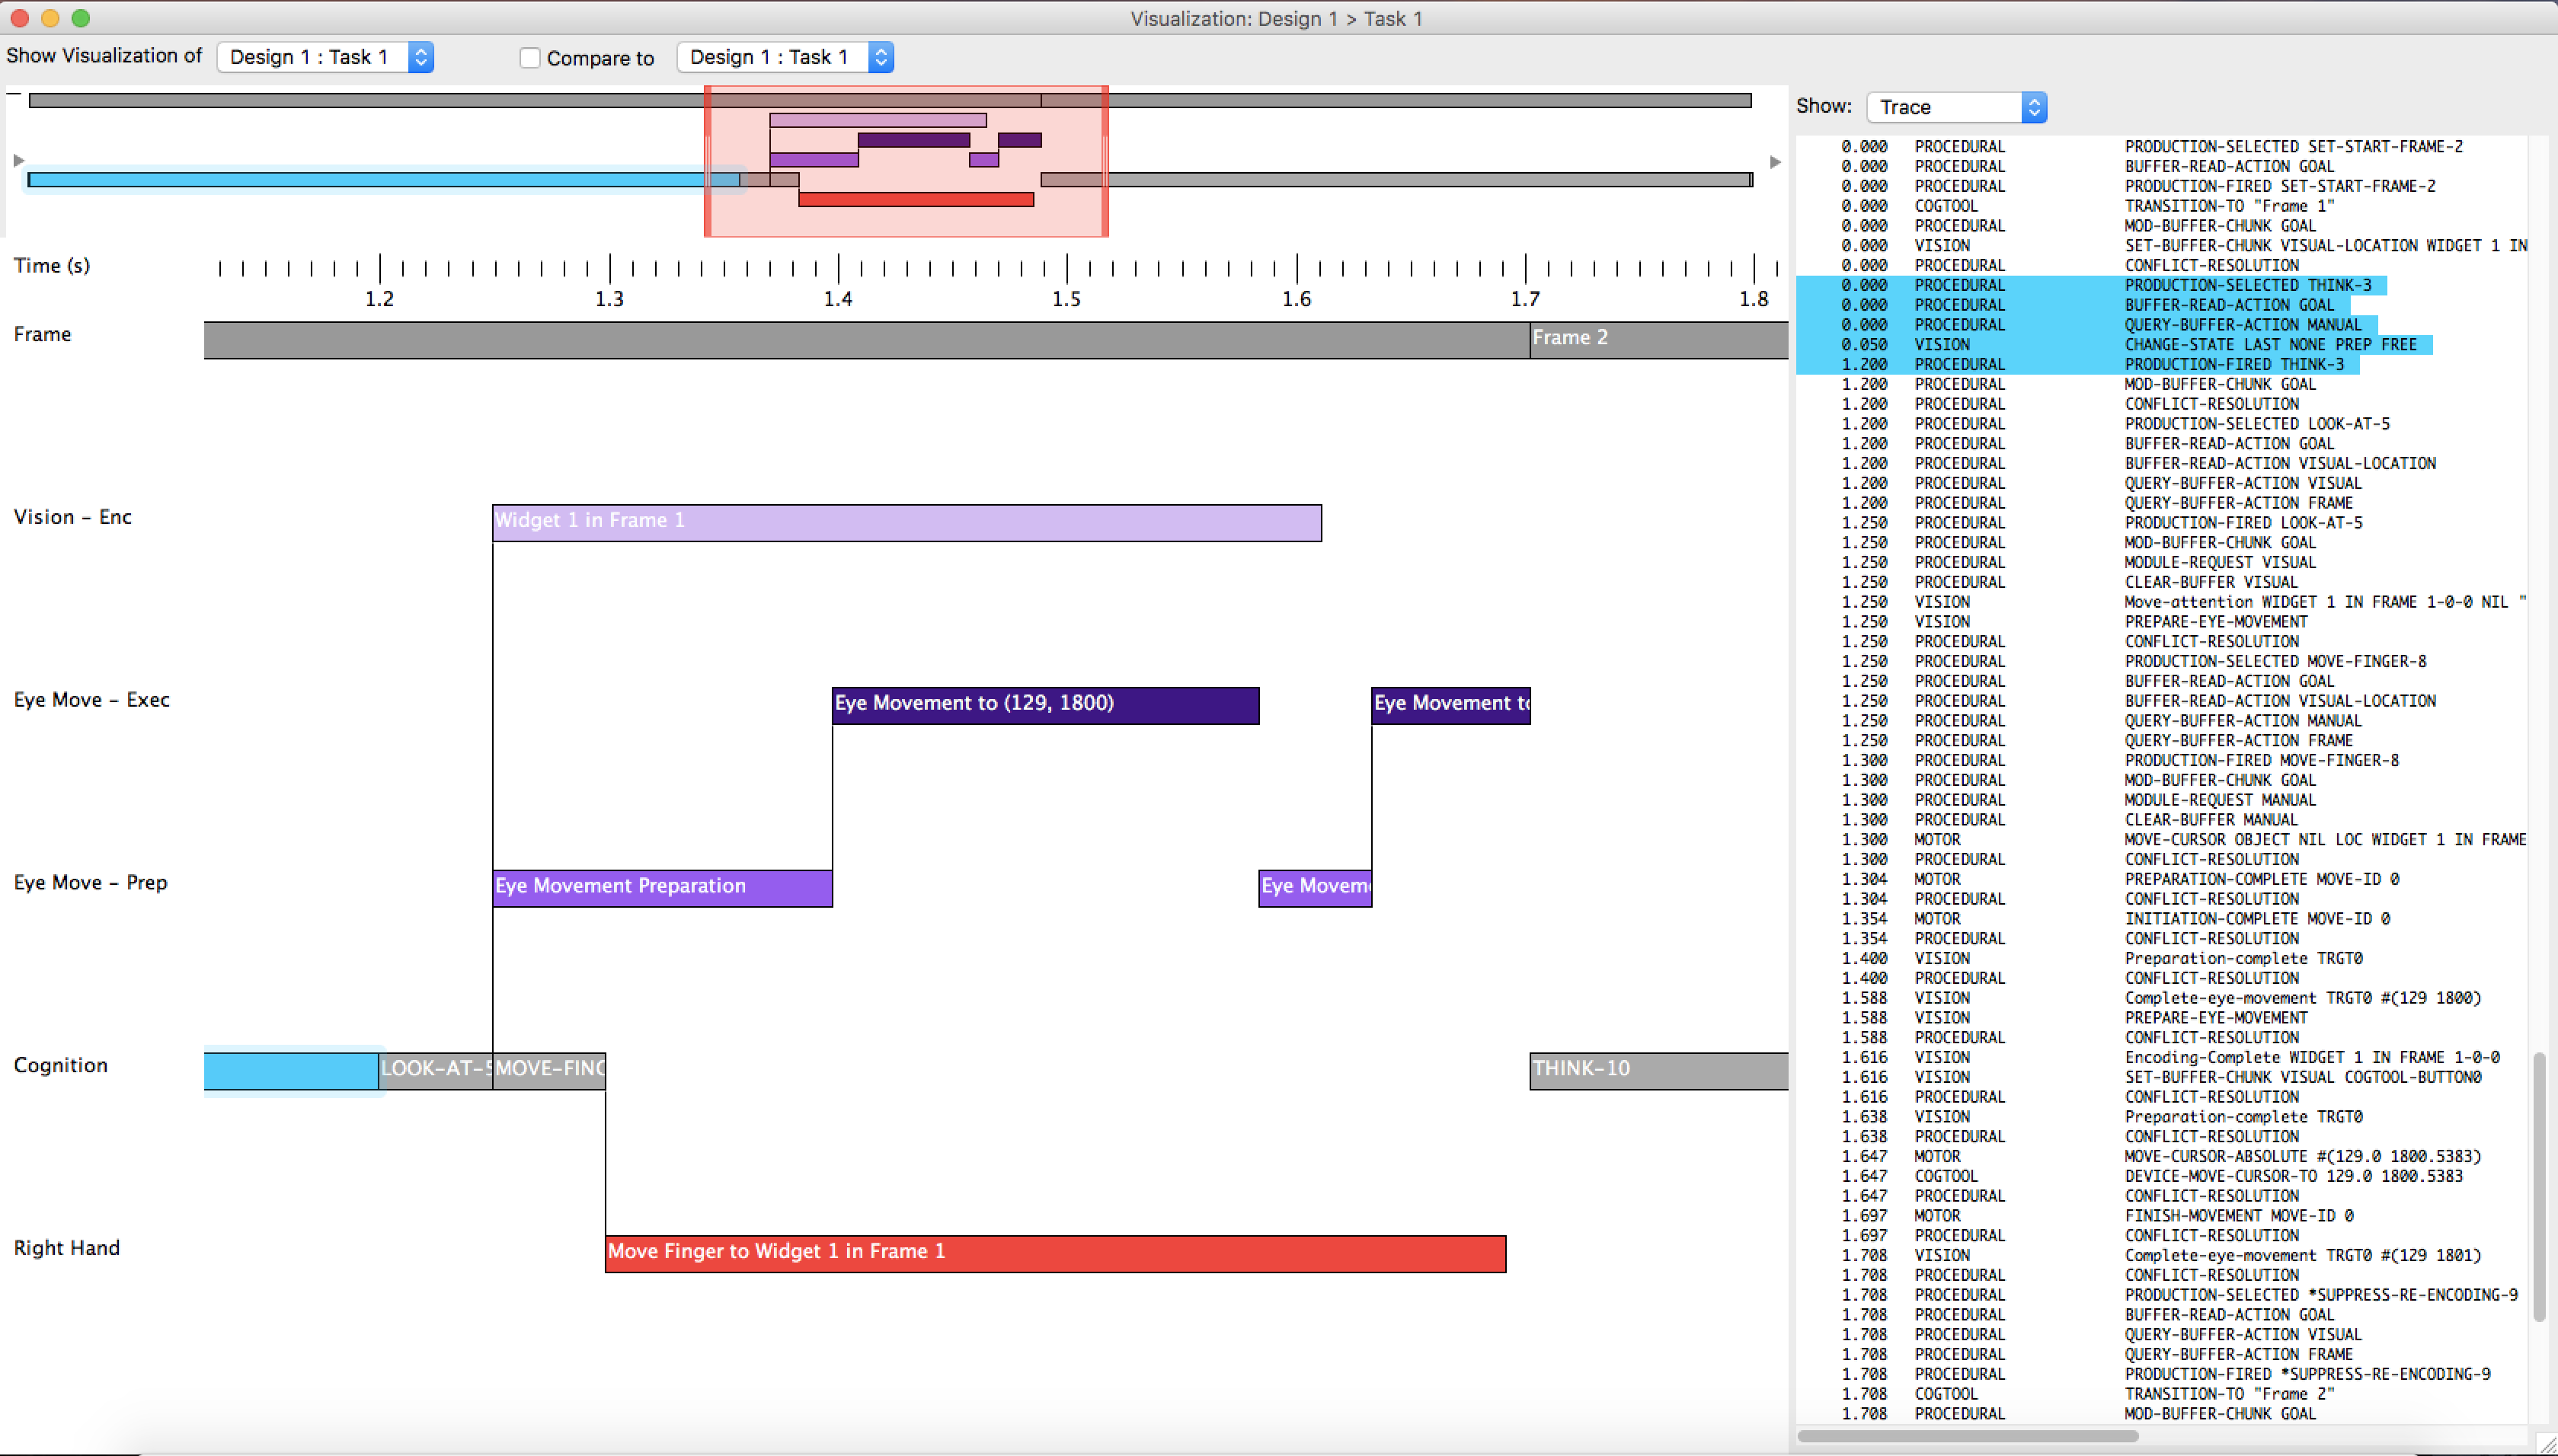
\includegraphics[scale=0.2]{CogToolVisualization}
    \caption{The highlighted part is the selected section of the user's action timeline.}
    \label{fig:cogtool-visual}
\end{figure}

The data presented by CogTool are useful for quickly evaluating the user experience of a system. It provides a quantitative model for analyzing the different tasks of a user and it can also be used for comparing different storyboards. This is helpful for designers to allow them to compare their design with competing designs \citep{bellamy2011deploying}.

% The data presented by CogTool are useful in evaluating the user experience of a system because it provides a quantitative model of analyzing the different tasks of a user and it can also be used for comparing different storyboards. This would be helpful especially for developers in determining whether a single line of code should already be written for an application based on the evaluated results.
        
        \subsubsection{Survey Instruments}

			Simple and easy to administer, surveys are one of the most commonly used methods of research \citep{goddard1996designing,mathers2007surveys}. Surveys can be used to gather information on individuals, given a set of questions. 
They are also frequently used to obtain information on user behavior and attitude \citep{mathers2007surveys}. Additionally, surveys may provide answers that may be generalized, depending on the way it was administered \citep{newsted1998survey}. 

		Surveys are good at finding out how many people do one thing or how many people think this way about something. However, they are limited in the sense that they fail to find out or answer why people do that one thing or why they think that way about something \citep{mathers2007surveys}. In cases like this, qualitative evaluation methods like focus group discussions are better at answering the ``why'' questions.
        
        Given that surveys are used to gather information on respondents' attitudes, several methods of measuring these have been developed. The most common one, however, is the Likert scale \citep{mcleod2008likert}. The Likert scale was developed by Rensis Likert in 1932 in order to provide a system for ``measuring'' the attitude of respondents. 
        
        Since then, the Likert scale has been commonly used as a five level scale measuring different levels of agreement or disagreement, frequency, importance, and likelihood on certain topics or concepts \citep{mcleod2008likert}. The advantage of this scale is that answers are not simply yes or no, and provide more insight on the attitude or behavior or the respondents \citep{likert1932technique,mcleod2008likert}.

	\subsection{Qualitative Evaluation}
    
		\subsubsection{User Acceptance Testing}
        
        The research will implement a mobile application for augmenting musical composition. To determine how effective the implementation of the system is, it will be tested on composers of varying skill. A method for getting feedback that would help identify issues in the application is User Acceptance Testing (UAT) \citep{davis2004toward}.
        
        %The research will implement a mobile application for augmenting musical composition. To determine how effective the implementation of the system is, it will be tested on composers of varying skill. A method to ensure that feedback is received that can be used to fix recurring issues or change any troubling detail in the application is through User Acceptance Testing (UAT) \citep{boltonuser}. 
        
        UAT can be used to measure the time it takes a user to finish a task, cognitive load, and their impression of the system after testing. These measures are seen in some experiments that performed user tests on similar systems like the touch-based system in the study of \citet{findlater2012beyond} where touch gestures and pop-up menus were the main features of the system. Music interaction research was also evaluated in the study of \citet{brown2017user} wherein it was found which factors were mostly used in testing, and how usability and aesthetics were the primary focus. These factors can be taken into consideration when planning the UAT for the system of the research.
        
        Before the UAT, there can be different tasks that can be designed for the user to accomplish based on the needs of the user. In evaluating music interaction research, \citet{brown2017user} enumerated the following categories of tasks given to participants:
        
        \begin{itemize}
        \item Specific Task
        \item Open Exploration
        \item Guided Exploration
        \item Watch Performance
        \item Prepare and/or Give Performance
        \item Workshop
        \item In The World Use
        \item Other
        \end{itemize}
        
        These categories can be used during the UAT of the system. There are also other concepts or methodologies that the group will consider when testing the system such as cognitive load through the use of CogTool, which was discussed in Section \ref{sec:cogtool}. These concepts can either be observed or used in conjunction with the UAT or they are implemented differently and individual from the UAT.
        
        	\paragraph{Think-Aloud Protocol}
            
            A concept that can be used during the UAT is the Think-Aloud Protocol. The Think-Aloud Protocol encourages the user to share their thought while performing tasks during the experiment. This protocol can help the user open up during the experiment and voice out whatever they are thinking whether it is their frustration with the system or their strategy when trying to complete a task \citep{gomoll1996some}. During testing, the user is reminded to constantly voice out their thoughts while completing tasks so that observations can include both actions and user motives \citep{gomoll1996some}. Although there is no specific standard followed by researchers in executing the Think Aloud Protocol \citep{mcdonald2013the,gill2012think}, there are still studies that provide guidelines such as the classical work of \citet{ericsson1998study} and augmented methods like the Explicit Think-Aloud (ETA) from the study of \citet{mcdonald2013the}.
            
            %A concept that can be used during the UAT wherein a user is encouraged to share their thoughts during the experiment is called the Think-aloud Protocol. This protocol can help the user open up during the experiment and voice out whatever their thinking whether its their frustration with the system or their strategy in trying to complete a task \citep{gomoll1996some}. During testing the user is reminded by the researchers to constantly voice out their thoughts while completing tasks so that observation can include both actions and user motives \citep{gomoll1996some}. Although there is no specific standard followed by researchers in executing the Think Aloud Protocol \citep{mcdonald2013the,gill2012think}, there are still studies that provide guidelines such as the classical work of \cite{ericsson1998study} and augmented methods like the Explicit Think-Aloud (ETA) from the study of \cite{mcdonald2013the}.
            
            In the work of \citet{ericsson1998study}, the Think-Aloud Protocol was mainly used during observation to detect problems as they occur. In this case, the information provided by the user must be validated due it being the user's own ideas and opinions \citep{ericsson1998study}. There are 3 guidelines provided in the study of \citet{ericsson1998study} to ensure the success of the Think-Aloud Protocol, these are: 
                       
            % In the work of \cite{ericsson1998study}, the Think Aloud Protocol was mainly used during observation to detect problems as they occur. Information provided by the user in this respect is important to be valid due to its nature of being from the introspection of the user \citep{ericsson1998study}. There are 3 classic guidelines provided by \cite{ericsson1998study} to ensure the validity of data verbalized by the user and to avoid the reactivity which can occur when any of these guidelines are violated. These guidelines are:
            
            \begin{itemize}
            \item A neutral instruction that does not request specific types of information
            \item A practice session
            \item A neutral ``keep talking'' reminder given by the researcher
            \end{itemize}
            
            The Think-Aloud Protocol was used in the study of \citet{yu2011probing} to better understand how students solve mathematical induction problems. These problems can be related to music as mentioned in the study of \citet{dorfler2001time}, where music has a complex set of features that are usually continuous in form. A musical composition can then be seen as a series of solutions to a mathematical problem. From this, the thought process of a composer can be captured using the Think-Aloud Protocol similar to the study of \citet{yu2011probing}.
            
            %The Think Aloud Protocol was used in the study of \citet{yu2011probing} to find out how a students solve mathematical induction problems specifically induction on infinite series. Using the Think Aloud Protocol \citeauthor{yu2011probing} was able to find more details of the students thought process while solving the problems. These problems can be related to music as mentioned in the study of \citet{dorfler2001time} wherein a complex set of features can be present within a composition usually infinite in form. This provides the relation of a composer composing music as a series of solutions as a mathematical problem as discussed by \citet{dorfler2001time} and the thought process of this problem solving by the composer can be captured by the Think Aloud Protocol as shown by \citet{yu2011probing}.
             
            
            %More? If yes. Add yu2011 if not then thank God.
            %Mention: Standards found in ericsson. Then compare? 
            %TF is meant to stitch the theory/study all together. Try being more direct with what we want for TAP in the context of the study. Why are we using TAP? What can it do in UAT? What can it do for music applications? -> Find more studies pointing at music as something that can be WOKE SHOOKT with vocal feedback. Find studies where saying things out loud/vocalization would improve music experience/provide more data for researchers because of the vocalization. MUSIC + TAP => ANO MERON? YAN POTA. FINISH THIS SHIT FAM
       
            \paragraph{Inspection}
            
            According to \citet{holzinger2005usability}, a usable application should have the following characteristics: (1) \textit{learnability}, meaning that the user should be able to learn how to use the system quickly; (2) \textit{efficiency}, so that the users can perform their tasks in an effective manner; (3) \textit{memorability}, which means it should be easy for users to use the system even after a long period of not using it (4) \textit{low error rate}, where the system should prevent users from committing errors; and lastly, (5) \textit{satisfaction}, meaning the system should be satisfying to use.  
            
            % One common and effective method of identifying and fixing user interface problems is through the use of usability inspection methods \citep{nielsen1994usability, porter1996review, fagan1999design, laitenberger2002survey}.
            
            One common and effective method of identifying whether an application has these characteristics is through the use of usability inspection methods \citep{nielsen1994usability, porter1996review, fagan1999design, laitenberger2002survey}. These are a set of methods that can be used to evaluate user interfaces and are usually in the form of heuristic evaluations, walkthroughs, and even mathematical theories of evaluation. 
            
            Inspection can be conducted during the UAT. One example of an inspection method is where the testers will not be provided help during the experiment, and are asked to navigate the application by themselves. This provides the users a natural environment, granting the test the most realistic result from users \citep{gomoll1996some}.
            
            \citet{nielsen1990heuristic} introduced the concept of heuristic evaluations, which is mentioned in Section \ref{sec:uist}. These are usually done by experts, evaluating whether the interface violates any of the said heuristics \citep{hollingsed2007usability}. It was found in a later study that this method found the most number of problems in a user interface compared to other methods \citep{jeffries1991user}.
            
            % Cognitive walkthrough
            In cognitive walkthroughs, the user will be given a goal to perform in the system. The evaluator or the person administering the test will then observe the steps or the actions the user will take to achieve that goal \citep{hollingsed2007usability}. These observations would help the developers and designers identify the pain points or the areas of confusion that the users experience within the application. 
            
            On the other hand, pluralistic usability walkthroughs allow inspection even without a fully developed user interface. Users are shown sketches of the screens on pieces of paper, where they will then identify the actions they would perform for each screen \citep{hollingsed2007usability}. This allows an easy method of usability inspection even in the early stages of development.
            
            These methods of inspection are widely used in development processes \citep{hollingsed2007usability}. There is no best method of inspection, as each method has its own strengths and weaknesses. Heuristic evaluations are quick and easy, but they could fail at identifying user needs. Both cognitive walkthroughs and pluralistic usability walkthroughs fix this problem, but can be time-consuming and representative rather than comprehensive depending on how the inspection was administered \citep{hollingsed2007usability}. However, it is common occurrence that these methods are used together to achieve better results that would benefit the study or the development goal.
            
            \begin{comment}
            \paragraph{Focus Group Discussion}
            
            %%FIX CITATION. WONGOWNGOWNGOWNGOWNGONGO
			Focus group discussions help provide a space for multiple target users and a moderator. This way, different perspectives can be understood by the researchers and learn different interpretations of the study through the discussions within the group \citep{wong2008focus}. Focus group discussions are not only a means to gain feedback from multiple respondents all at once but to discover new pieces of information brought about discourse and interaction between each person in the group whether it be through arguments or agreements \citep{kitzinger1994methodology}. 
            
             According to the study of \citet{kitzinger1994methodology}, focus group discussions are an effective way to develop an idea between participants within an atmosphere dictated by the backgrounds of each participant. \citet{kitzinger1994methodology} also mentioned that important interactions happen during focus group discussions and that these interactions can increase based on the variety of the background of the participants. 
            
            For example, both the studies of \citet{wong2008focus} and \citet{kitzinger1994methodology} was within the domain of health and medicine. Through the focus group discussion, both arrived at the conclusion where the data gathered was highly relevant to the context behind the study. This was due to how the users were able to voice out their concerns, paint points, and ideas.
            
            %For example, both the studies of \citet{wong2008focus} and \citet{kitzinger1994methodology} was within the domain of health and medicine. and both arrived at the conclusion where the data gathered during focus group discussion was highly relevant to the context behind the study.
                    
           % As music is already embedded within the culture of modern society either through the entertainment it brings \citep{hawkins2013pac,donnelly2005spectre} or the benefits it has on psychological health \citep{kemper2005music}, focus group discussion on music can bring interactions between a wide variety of individuals due to the familiarity of music. The concepts found in music is also personal to composers. The process of composition can ask for a heavy investment on composers where multiple iterations can occur before arriving at the final draft which can take time and resources from the composer \citep{bennett1976process}. Composing music can also be a personal endeavor for composers who add their own style into their compositions \citep{rothgeb1975strict, miller1984genre}.
            
           
            As music is already embedded within the culture of modern society either through the entertainment it brings \citep{hawkins2013pac,donnelly2005spectre} or the benefits it has on psychological health \citep{kemper2005music}, focus group discussion on music can bring interactions between a wide variety of individuals due to the familiarity of music.     
            
            Composers are personal with their music and each composition has a special standard stemming from the background of the composer \citep{rothgeb1975strict,miller1984genre}. However, it was found in the study of \citet{folstad2008effect} that group discussions yielded better results for usability inspection and evaluation compared to individual inspection. This potentially means that focus group discussion conducted with multiple composers would yield more ideas and better results.
            
            %According to the study of \citet{kitzinger1994methodology}, focus group discussions are an effective way to develop an idea between participants within an atmosphere dictated by the backgrounds of each participant. \citet{kitzinger1994methodology} also mentioned that important interactions happen during focus group discussions and that these interactions can increase based on the variety of the background of the participants. Composers are personal with their music and each composition has a special standard stemming from the background of the composer \citep{rothgeb1975strict,miller1984genre}. Additionally, the study of \cite{folstad2008effect} looked into the concept of group discussions that looked into the Usability Inspection of a website and yielded better results compared to individual inspection. This potentially means that focus group discussions conducted between composers can provide better data in designing a usable mobile composition tool.
            \end{comment}
            
            

\section{Musical Composition and Its Systems}
	\subsection{Musical Composition}
    	\subsubsection{The Composition Process}
       
       The theories involving the creative process, specifically musical composition, was explored in the study of \citet{collins2005synthesis}. In this study, four (4) theories were mentioned, these were: (1) stage theory, (2) Gestalt theory, (3) emerging systems theory, and (4) information processing theory. It was noted, however, that the Gestalt theory was the most evident in application in the musical composition process.
       
       The Gestalt theory divides the process into different sub-parts that would eventually combine in the end to form the composition. Its main essence is the restructuring phase of the process, also known as `the flash of illumination' \citep{collins2005synthesis}. This phase is described as an instance during the process where the composer experiences an unexpected solution to the problem or obstacle and uses it to progress further in completing the composition.
       
        %The general theories of the creative process was explored in composing music by \citet{collins2005synthesis}. He mentioned four theories namely, stage theory, Gestalt theory, emerging systems theory, and information processing theory. However the results from the work of \citet{collins2005synthesis} portrays the Gestalt theory being the most evident when applied to composing music compared to the other theories mentioned. This theory focuses on the process divided into different sub-parts and combined in the end to create the final product. The main essence of this theory is the restructuring part of the process also known as the 'flash of illumination' \citep{collins2005synthesis}. This part is described as an instance during the process in where the composer experiences an unexpected solution to the problem and uses it in order to progress further in completing the musical composition.
        
        \begin{comment}
        \begin{figure}[H]
			\centering
			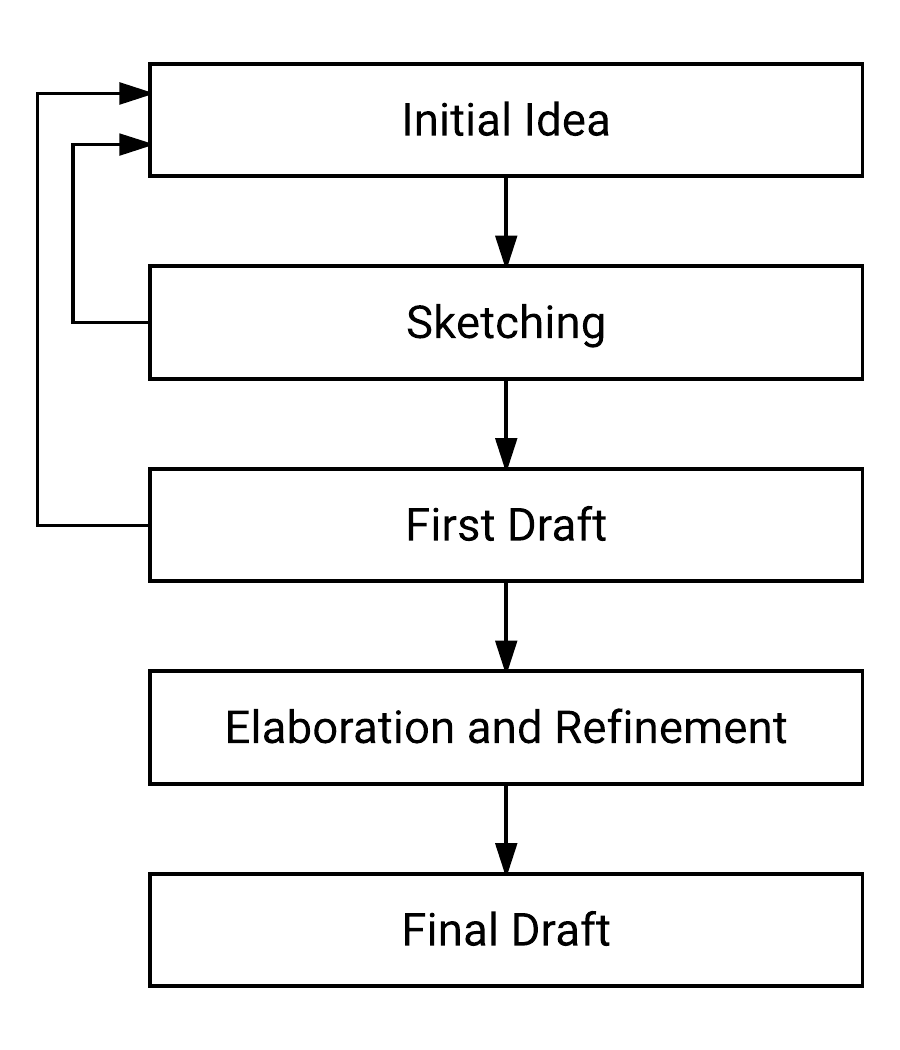
\includegraphics[scale=0.2]{Process_of_Composition}
    		\caption{The stages of music composition. \citep{bennett1976process}} 
    		\label{fig:MUSIC_benettcompositionstages}
		\end{figure}
        \end{comment}
        
        The earlier study of \citet{bennett1976process} reflects the Gestalt theory. It was highlighted in the study that the composition process involved various stages (see Figure \ref{fig:composing-graph}). A composition starts off with a germinal or initial idea for the theme or motif of the composition \citep{bennett1976process,collins2005synthesis}. Once a motif is in mind, the composer moves on to the sketching phase. However, it is still possible for the composer to go back to the ideation stage, even if a draft has already been completed if the composer feels the need for a revision or an unexpected idea comes up. This is what \citet{collins2005synthesis} calls \textit{backtracking}, where the composer goes back to previous stages of the process to reformulate ideas or segments of a draft.
        
        The drafts go through a lot of refinement and revisions as long as the composer is not satisfied with the output \citep{bennett1976process}. Even with the idea in mind, some pieces of the draft might still be improved to better fit the composition. This phase is similar to that of the recurring restructuring stage defined in the study of \citet{collins2005synthesis}. This restructuring involves reformulating pieces of the composition to achieve the final draft. 
        
        % In connection with the Gestalt theory, \citet{bennett1976process} expressed the compositional process in various stages (seen in Figure \ref{fig:MUSIC_benettcompositionstages}) still reflects the Gestalt theory. It starts off at the germinal ideation for the theme or motif from the composer, much like in the process discussed in the study of \citet{collins2005synthesis}, and moves to the sketching period. However the sketching stage and the first draft stage can still go back to the germinal ideation stage for a sudden revision or an unexpected solution encountered by the composer. After the final draft, \citet{bennett1976process} described the last stage of composing as 'Revisions?'. With that said, uncertain or unexpected revisions can be discovered even after the final draft is done. These instances of backtracking can be compared to the recurring restructuring stage from the process discussed by \citet{collins2005synthesis}. It involves reformulating the givens and goals in order to achieve sub-goals. All in all, numerous revisions and restructuring are done in composing music in order to achieve the desired product by the composer.
        

        
        \begin{comment}
      
        %%% Discuss the motif, the main theme of music %%%
        
        Composers often start off with a certain sequence of notes that dictate the theme of their musical composition, this is called the motif. This is the repeating series of notes that occur in different parts of the musical composition. It is also often used to create the last song syndrome (LSS) in most of the songs today.
        
        %%% How the song revolves around the motif using various melodic intervals %%%
        
        From the motif, the composer can then use chord progressions or melodic intervals in order to expand the composition with respect to music theory. However, composers would have to choose those creatively in order to set the mood or emotion that the composition or song wants to portray to listeners.
        
        %%% Mention how composers usually copy paste and transpose or elongate or invert notes %%%
        
        With the recurring theme in the composition, composers are faced with the problem of imitating the motif throughout different parts of the song. Copy pasting is often used in musical notation softwares in order to achieve this. However tweaking through transposing, elongation, or inverting the motif is also evident in order to build variation in delivering the motif in compositions.
        
        \end{comment}
        
        \subsubsection{Concepts}
        
        \paragraph{Fundamentals of Music}
        
        Music cannot be taught without knowing the fundamentals first, namely: pitch and melody, rhythm, texture and harmony, color and timbre, and form or design \citep{rivadelo1986fundamentals}. By combining all of them, they form into what is known today as music \citep{willoughby1971comprehensive}.
        
        %By intertwining them all, it builds into, what we know today, Music \citep{willoughby1971comprehensive}.

Music is mainly formed by several notes or rests in a sequence. A consecutive progression of notes that are relative to each other is called the melody \citep{rivadelo1986fundamentals}. In Paul Hindemith’s theory of melody, melody is considered as the element of a composition that truly reveals the personality of the composer \citep{cheng2016approaching}. 

Pitch is defined as the highness or lowness of a tone or musical sound relative to the amount of vibrations per second \citep{rivadelo1986fundamentals}. Each pitch is represented by the first seven letters in the alphabet, which are A, B, C, D, E, F, and G \citep{miller2005complete}. However, the distance of a pitch from each other can be described as a whole step and a half step or semitone. The distances can be easily derived from the keys of a piano or keyboard. Moving from one key to a next key is called half step or semitone respectively. A whole step on the other hand is described as moving from one key to another by skipping a key between them. Both can be used to traverse forward and backward by adding the word up or down after the distance. Multiple steps can also be achieved by putting a number before the distance.

The pitch can also be represented using the Solfeggio Method, commonly known as the Do-Re-Mi. However, the same pitch representation may also be found on higher or lower tones which are divided by an octave, which is a fixed interval between pitches.

Another element of music is the duration, which is the amount of time a tone lasts \citep{rivadelo1986fundamentals}. The duration is shown in a composition through the use of different notes or rests that indicate the duration of a certain pitch \citep{rivadelo1986fundamentals, burrows1999reading}. More of this will be discussed in Section \ref{sec:musical_notation}.

% Pitch is defined as the highness or lowness of a tone or musical sound which is ascertained by the amount of vibrations per second \citep{rivadelo1986fundamentals}. Each pitch is represented with the first seven letter in the alphabet which is A, B, C, D, E, F, and G \citep{miller2005complete}. They can also be represented using the Solfeggio Method which is commonly known as the Do-Re-Mi. However, the same pitch representation can also be found on higher or lower tones which are divided by an octave which is a fixed interval between pitches.

In a composition, \citet{rivadelo1986fundamentals} mentions that rhythm represents the pace of the musical flow through the common patterns that currently exist. It can be understood as the factor that makes musicians and composers aware of the beat or tempo of composition. It allows them to align their ideas in order to create music on top of the rhythm. 

Rhythm also consists of 4 parts, which are: beat, accent, meter, rhythmic pattern, and phrase \citep{rivadelo1986fundamentals}. The beat is the basic time unit of the composition. The accent forms the theme of the rhythm, while the meter divides the beats into sections. The rhythmic pattern groups the beats to form a coherent pattern of sound. Finally, the phrase is considered as the musical thought, that is a part of the whole musical sentence.

% In a whole composition, \citet{rivadelo1986fundamentals} mentioned that rhythm represents the musical flow’s pace through the common patterns that currently exist. She also stated that “it is the principle that enables one to organize or to bring order into their perception of time and space”. It can be derived that it makes musicians and composers aware of the beat or tempo for them to align with it their ideas in order to create music on top of the rhythm, based on what she said. Rhythm also consists of 4 parts having: beat, accent, meter, rhythmic pattern, and phrase \citep{rivadelo1986fundamentals}. With the beat being the time unit, the accent forming the beats into parts, the meter dividing the beats into sections, the rhythmic pattern grouping the beats to form patterns of sound, and phrase being “the musical thought that is a part of the musical sentence“.



% Consecutive progression of notes that are relative with each other is called Melody \citep{rivadelo1986fundamentals}. In Paul Hindemith’s theory of melody, “melody is the element in which the personal character of the composer is clearly and cleverly revealed” \citep{cheng2016approaching}. Pitch and duration, the amount of time a tone lasts, are the basic properties according to \citet{rivadelo1986fundamentals}. It also has 5 properties that make music different from each other namely: Rhythm, Dimension, Direction or Movement, Progression, and Register. The dimension contains the length and range of a melody. The length, from the term itself, is the measurement of the melody, it can be short or long. The range is the distance of the highest and lowest sound or tone.
        
        \paragraph{Basic Music Theories}
        
        Knowledge of music theory can aid a musician to compose music without having to waste time thinking about succeeding notes or melodies. According to \citet{meyer1989style}, it can be likened to rules or guidelines that can change over time due to changes in cultural style. The theories in music also utilize some of the fundamentals of music to create these guidelines. It assembles the basic fundamentals into a harmonic structure that characterizes and builds music \citep{meyer1989style}.
        
        % Music Theories can aid a musician to compose good music without relying on too much memorization. It can be related to arbitrary rules, as stated by \citet{meyer1989style}, that change over time due to the change in culture. It can also be described to govern music that make songs sound good. The theories in music also utilize some of the fundamentals of music in creating the said arbitrary rules. It assembles the basic fundamentals into a harmonic structure that characterizes and builds into as to what is music today.
        
        There are multiple concepts in music theory that can start off a musician to compose his or her own music piece. Although music theory can serve as a guide for composition, it is not an all-in-one solution. Composers will still have to think creatively to identify which theories are applicable or could be applied in the current composition \citep{meyer1989style}. Some form of trial-and-error would still be present in this process.
        
        %However this may guide the composer in composing music, it is not a all-in-one solution in composing a whole composition. Composers still have to think creatively which theories or part of a theory is most applicable in his or her composition. The trial-and-error process in musical composition would still be present.
        
        Tetrachords are one of the most frequenly used concepts in music theory \citep{spencer1996music}. They are four succeeding notes that form a structure that dictates the perfect fourth of the first note. \citet{spencer1996music} stated 4 kinds of tetrachords: major, minor, natural, and harmonic. They are differentiated by the number of semitones being skipped relevant to the first note. Major follows the pattern 2-2-1 semitones, minor goes 2-1-2, natural uses 1-2-2, and lastly, harmonic follows 1-3-1. 
        
        
        Scales can then be derived from tetrachords \citep{spencer1996music}. Combining two (2) tetrachords and adding a whole step or a tone in the middle of the two tetrachords would result in a scale. For example, two major tetrachords (2-2-1) with a whole step in the middle would result in: 2-2-1-(2)-2-2-1, which is actually the major scale.
        
        %Tetrachords and scales are the first to be discussed by \citet{spencer1996music} as it is going to be used frequently in music theory is a whole. Tetrachords are four succeeding notes that form a structure that dictates the perfect fourth of the first note. \citet{spencer1996music} stated 4 kinds of tetrachords, Major, Minor, Natural, and Harmonic. They are simply explained by showing the number of semitones that you have to skip in order to build the tetrachord based from the first note desired by the composer. Major follows the pattern 2-2-1 semitones, minor goes 2-1-2, natural goes 1-2-2, and lastly, harmonic follows 1-3-1. Scales can be derived with the help of tetrachords. Multiplying two tetrachords and adding a whole step or a tone in the middle of the two semitones forms a scale. For example, two major tetrachords with a whole step or a tone in the middle, 2-2-1-(2)-2-2-1, forms the major scale.
        
        There are certain harmonic intervals that composers can utilize to build a good musical composition \citep{spencer1996music}. These are called melodic intervals. They can be described as various note sequences that composers can use in their composition to build the motif or the whole composition as a whole \citep{spencer1996music}. 
        
        There are two characters used to distinguish intervals from each other. The first character denotes the quality of the interval \citep{spencer1996music}. This can be any of the letters: M, P, m, d, A. M is described as a major interval, P as a perfect interval, m as a minor interval, d as diminished, and A as augmented. Each of these intervals give off different sounds for the note sequences they produce \citep{spencer1996music}.
        
        The second character is about the quantity of an interval. It is a number which identifies the length of the interval or the distance of one note from another \citep{spencer1996music}. However, not all interval qualities contain all interval lengths. Some may contain the same numbers from another melodic interval but they are different in terms of how many semitones are skipped in order to dictate the next note.
        
        % There are certain intervals that are described as harmonic \citep{spencer1996music} that composers can utilize in order to build a good musical composition, they are called melodic intervals. They can be described as various note sequences that composers can use in their composition in order to build the motif or the whole composition as a whole. There are two characters in distinguishing an interval from each other. The first character is the quality of the interval which are the letters, M, P, m, d, A. M is described as a major interval, P as a perfect interval, m as a minor interval, d as diminished, and A as augmented. Each of this interval gives off a different sound when listening to the note sequences it produces. The second character is a number which is the length of the interval or the distance of one note is from the other. However, not all interval qualities contain all interval lengths. Some may contain the same numbers from another melodic interval but they are different in terms of how many semitones are skipped in order to dictate the next note.
 
\begin{comment}

\begin{figure}[H]
\centering
\begin{minipage}{.4\textwidth}
	\centering
	\includegraphics[width=.7\linewidth]{major_triad}
    \caption{Major Triad}
    \label{fig:major_triad}
\end{minipage}
\begin{minipage}{.4\textwidth}
	\centering
	\includegraphics[width=.7\linewidth]{minor_triad}
    \caption{Minor Triad}
    \label{fig:minor_triad}
\end{minipage}
\end{figure}

\begin{figure}[H]
\centering
\begin{minipage}{.4\textwidth}
	\centering
	\includegraphics[width=.7\linewidth]{augmented_triad}
    \caption{Augmented Triad}
    \label{fig:augmented_triad}
\end{minipage}
\begin{minipage}{.4\textwidth}
	\centering
	\includegraphics[width=.7\linewidth]{diminished_triad}
    \caption{Diminished Triad}
    \label{fig:diminished_triad}
\end{minipage}
\end{figure}

\end{comment}

\begin{figure}[H]
	\centering
	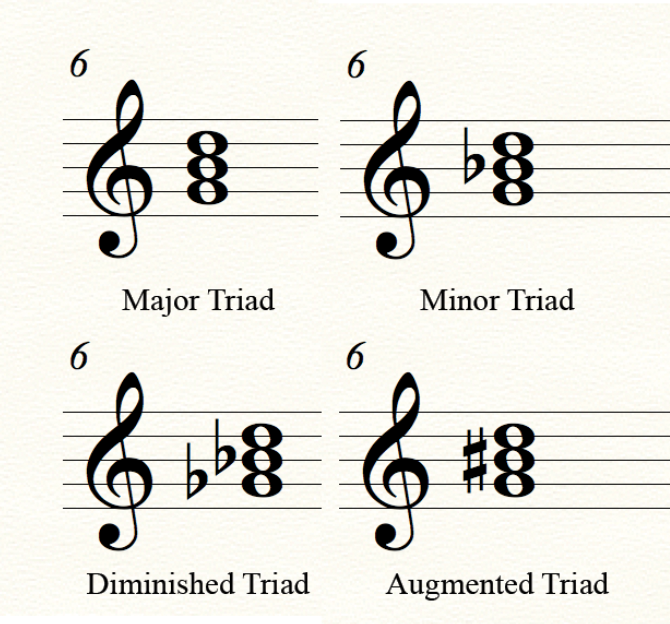
\includegraphics[scale=0.5]{triads}
    \caption{Various triads \citep{spencer1996music}.}
    \label{fig:MUSIC_triads}
\end{figure}
        
        The basic chords in a musical composition are defined by triads. It is basically three notes that are played simultaneously. Like tetrachords, there are four types of triads: major, minor, augmented, and diminished \citep{spencer1996music}. Figure \ref{fig:MUSIC_triads} show the various triads in a musical composition. The lowest note in the triad is called the root, the middle note being the third, and the highest note is called the fifth. However, triads have different qualities in different scales, specifically the major scale, natural minor scale, melodic minor scale, and the harmonic minor scale. In these scales, triads are classified into scale degrees which are like roman numerals which are both lower-case and upper-case. These scale degrees are often used in defining different chord progressions.
        
        
        \paragraph{Musical Notation}
        \label{sec:musical_notation}
        
        The modern notation system in music today, specifically western musical notation, was derived from places where the western culture continued to thrive \citep{read1969music}. However, the practice of writing musical notation did not originate from western culture \citep{read1969music}. Musicologists discovered that pre-Christian Greeks have already been using musical notation, and have developed four (4) unique systems for writing them \citep{read1969music}. Nonetheless, the modern musical notation system holds some similarity to the system developed in the past. 
        
        %The modern notation system in music today, specifically western musical notation, were derived from places where the western culture continued to thrive \citep{read1969music}. However writing musical notations were not originated from the western culture, \citet{read1969music} mentioned that musicologists discovered that pre-Christian Greeks have known musical notation and has four unique systems for writing them. Nonetheless, some resemblances in practice from the past notation system can also be seen in the modern system.
        
        According to \citet{read1969music}, musical notation is known as a method for visually representing musical sound. It is what musicians use to graphically display their musical ideas and can be read by other musicians as well. In relation to writing and reading any character in any language, it also requires understanding of the symbols used in music notation in order to be literate in music \citep{read1969music}. 
        
        %"the visual manifestation of the interrelated properties (or fundamentals) of musical sound". It is what musicians used to graphically display their musical ideas and can be read by other musicians as well. In relation to writing and reading any character in any language, it also requires you to understand the symbols used in music notation in order to be literate in music.
        
\begin{figure}[H]
	\centering
	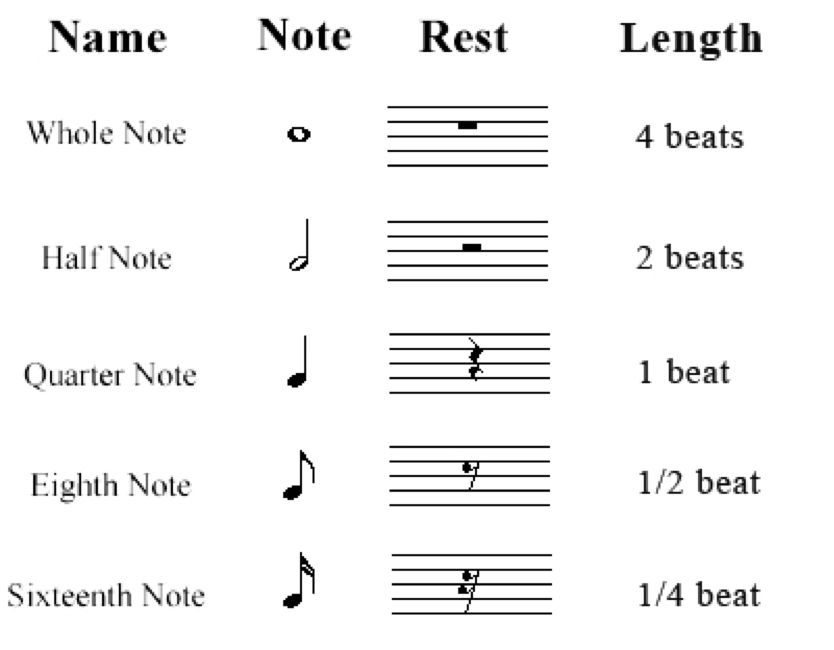
\includegraphics[scale=0.2]{BasicNoteRest}
    \caption{Basic notes and rests used in modern musical notation \citep{riso2016basic}.}
    \label{fig:MUSIC_basic-notes-rests}
\end{figure}
        
        The basic symbols in musical notation are the notes and rests seen in Figure \ref{fig:MUSIC_basic-notes-rests}. These are found throughout the staff, which is the set of lines and spaces that represent the different levels of pitches. Beams are the black bars that are used to group consecutive notes that are less than a quarter note in order to improve the visualization of the composition itself \citep{spencer1996music}. However, the pitches that represent each space or line in the staff is different based on the clef used at the start. The G-Clef or treble clef and the F-Clef or bass clef (see Figure \ref{fig:MUSIC_gclef_fclef}) change the pitch representations on each line and space on the staff. When the G-Clef is used at the start of the staff, each line starting from the bottom represents the pitches E-G-B-D-F and spaces represent the pitches F-A-C-E. On the other hand, when the F-Clef is used at the start of the staff, each line starting from the bottom represents pitches G-B-D-F-A and the spaces represents the pitches A-C-E-G.
        
\begin{figure}[H]
	\centering
	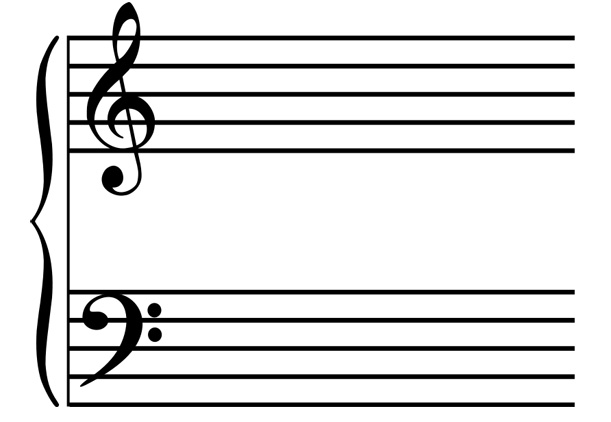
\includegraphics[scale=0.2]{G-ClefAndF-Clef}
    \caption{The G-Clef and F-Clef \citep{stamp2013the}.} 
    \label{fig:MUSIC_gclef_fclef}
\end{figure}

	There is only one element in musical notation that indicates the distinct rhythm throughout the composition, and that is the time signature \citep{rivadelo1986fundamentals}. There are two numbers in the time signature, (see Figure \ref{fig:MUSIC_timesignature}) called the numerator and the denominator. When writing the time signature, the numerator takes up the upper two spaces of the staff while the denominator takes up the lower two spaces of the staff \citep{read1969music}. Each part of the time signature defines the notes to be used in the musical composition. The numerator or the upper number denotes the amount of beats in one bar or measure while the denominator or the lower number indicates the type of note that would equal to one beat \citep{read1969music, rivadelo1986fundamentals,burrows1999reading}.

	% There is one element in musical notation that initializes the distinct rhythm throughout the composition \citep{rivadelo1986fundamentals}, and that is the time signature. There are two numbers in the time signature, seen in Figure \ref{fig:MUSIC_timesignature}, called the numerator and the denominator. In the staff, the numerator takes up the upper two spaces of the staff while the denominator takes up the lower two spaces of the staff \citep{read1969music}. Each part of the time signature defines the notes to be used in the musical composition. According to \citet{rivadelo1986fundamentals}, \citet{read1969music}, and \citet{burrows1999reading}, the numerator or the upper number denotes the amount of beats in a bar or measure while the denominator or the lower number indicates the type of note that would be tantamount to a beat.
    
\begin{figure}[H]
	\centering
	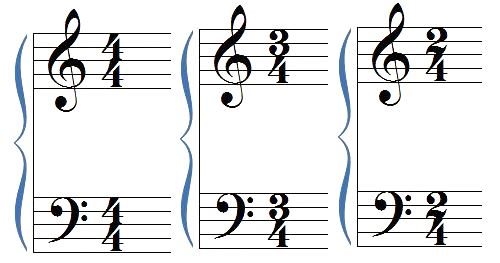
\includegraphics[scale=0.4]{Time-Signature}
    \caption{Various time signatures \citep{rose2014reading}.} 
    \label{fig:MUSIC_timesignature}
\end{figure}

A series of notes in a musical sheet is divided by bar lines (see Figure \ref{fig:MUSIC_barlines}). However, there are two kinds of bar lines in musical pieces. The first is the simple bar line which is one vertical line that divides a series of notes based on the time signature. The second type of bar line is the double bar line which is made up of two vertical lines. It specifies the end of a part in a music composition \citep{read1969music}. This is where composers can change the time signature and key signatures of the current staff. However there are variations to the double bar. The first is the one that signifies the end of the composition which is the ``period'' form \citep{read1969music} or final bar line. This kind of bar line is found at the end of the composition. The other two variations are double bars that work together, they are the start repeat and the end repeat. It encloses a number of bars between the start and end repeat which sums up the number of beats as a whole that would satisfy the time signature declared before the start repeat bar.
    
\begin{figure}[H]
	\centering
	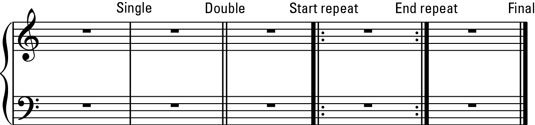
\includegraphics[scale=0.4]{barlines}
    \caption{The different bar lines \citep{dummy2017barlines}.} 
    \label{fig:MUSIC_barlines}
\end{figure}

There are certain annotations that are used to dictate the strength of the sound of notes, these are called dynamics. Shown in Figure \ref{fig:MUSIC_dynamic} are several levels of dynamics that can be used in musical compositions. These markings can be usually found above or below the notes that are affected by the dynamic marking \citep{read1969music}. However, there are symbols that also complement dynamic markings, which are called dynamic signs. 

Crescendo and diminuendo or decrescendo are the only dynamic signs. Both signs are used when a succession of notes is gradually increasing or decreasing to a certain dynamic. The example shown in Figure \ref{fig:MUSIC_dynamicsignsmarkings} exhibits the use of both signs. Basically, crescendo is when the loudness increases up to a certain dynamic and decrescendo is when the loudness decreases down to a certain dynamic. In Figure \ref{fig:MUSIC_dynamicsignsmarkings}, crescendo is used when the loudness of the notes increased from mezzo forte to forte. Decrescendo is used when the loudness of the notes descended from forte to mezzo forte.

	% There are certain annotations that are used in order to dictate the strength of sound of the notes, it is called dynamics. In Figure \ref{fig:MUSIC_dynamic}, there are several levels of dynamics that can be used in musical compositions. These markings can be usually found above or below the notes that are affected by the dynamic marking \citep{read1969music}. However, there are symbols that also complement dynamic markings which are dynamic signs. Crescendo and diminuendo or decrescendo are the only dynamic signs. Both signs are used when succession of notes are gradually increasing or decreasing to a certain dynamic. An example in Figure \ref{fig:MUSIC_dynamicsignsmarkings} exhibits the use of both signs. Basically, crescendo is when the loudness increases up to a certain dynamic and decrescendo is when the loudness decreases down to a certain dynamic. From Figure \ref{fig:MUSIC_dynamicsignsmarkings}, crescendo is used when the loudness of the notes increased from mezzo forte to forte. Decrescendo is used when the loudness of the notes descended from forte to mezzo forte.
    
\begin{figure}[H]
	\centering
	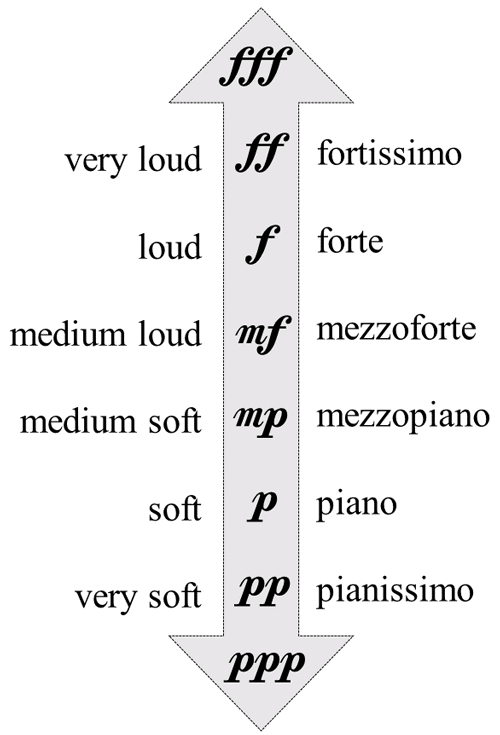
\includegraphics[scale=0.2]{dynamic_markings}
    \caption{The various dynamic markings \citep{peter2016dynamic}.}
    \label{fig:MUSIC_dynamic}
\end{figure}

\begin{figure}[H]
	\centering
	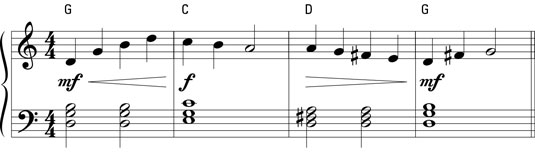
\includegraphics[scale=0.4]{dynamic_signsandmarks}
    \caption{Dynamic markings and signs \citep{dummy2016volume}.}
    \label{fig:MUSIC_dynamicsignsmarkings}
\end{figure}
 
        \paragraph{Circle of Fifths}
        
\begin{figure}[H]
	\centering
	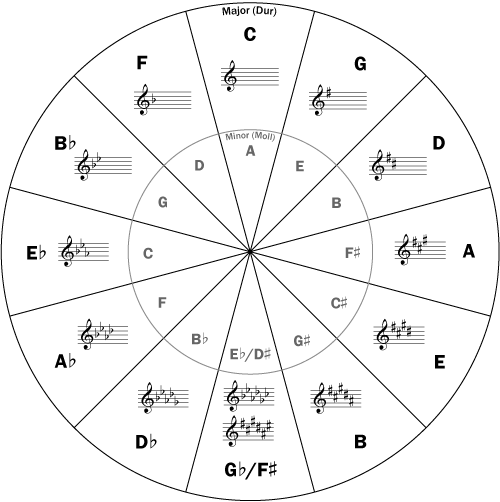
\includegraphics[scale=0.5]{circle-of-fifths}
    \caption{The circle of fifths \citep{gleaves2015understanding}.}
    \label{fig:MUSIC_circleoffifths}
\end{figure}
        
        The circle of fifths (see Figure \ref{fig:MUSIC_circleoffifths}) was derived from the the Pythagoras Circle made by famous Greek philosopher Pythagoras \citep{jensen1992circle}. It was later expanded in the work of Nikolai Diletskii on amplification and Johann Heinichen's work on modulation \citep{jensen1992circle}. It is also now commonly used today as a basis for teaching techniques in composing and playing music. Some of these techniques include modulation and chord progressions. %Nonetheless, the circle of fifths requires a few amounts of time in order to learn how to read and utilize it.
        
         It can be compared to a 12-hour round clock with the numbers replaced by the names of different pitches (see Figure \ref{fig:MUSIC_circleoffifths}). All of the succeeding pitch representations going clockwise starting from C are derived from the fifth of the previous pitch \citep{jensen1992circle}. For example, starting from C, the fifth of C would be G, and the fifth of G would be D and so on. It would revolve back to C when it reaches F. The inner circle is a copy of the outer circle only moved counter-clockwise twice.
        
       % It can be compared to a 12-hour round clock with the numbers replaced by the names of different pitches. Each number in the clock also represents a pitch representation as seen in Figure \ref{fig:MUSIC_circleoffifths}. All of the succeeding pitch representations, clockwise from C, is derived by the fifth of the previous pitch. For example, starting from C, the fifth of C would be G, and the fifth of G would be D and so on. It would revolve back to C when it reaches F. The inner circle is a copy of the outer circle only moved counter-clockwise twice.
        
        Although it may look like a clock, counting with the circle of fifths is different. It starts at 0 from the top or north and both sides (clockwise and counter-clockwise) count from 1 and end at 6 at 6 o'clock. Those numbers denote the key signatures that are present in a major or minor scale in a musical composition \citep{jensen1992circle}. Key signatures are derived from the circle of fifths through the counting. The sharps in the key signature begin counting clockwise at F and flats begin counting counter-clockwise at B \citep{clough1986musical}.
        
        %Although it may look like a clock, counting with the circle of fifths is different as it starts at 0 from the top or north and both sides (clockwise and counter-clockwise) counts from 1 and ending at 6 at 6 o'clock. Those numbers denote the key signatures that are present in a major or minor scale in a musical composition. Key Signatures are derived from the circle of fifths with the help of counting with the use of the numbers. The sharps in the key signature begin counting clockwise at F and flats begin counting counter-clockwise at B.
        
        %%% Discuss how chords are derived from the circle %%%
        
        From the circle of fifths, major triads can be derived \citep{jensen1992circle, spencer1996music}. This can be done by choosing a root note from the outer circle, then getting its third and fifth \citep{jensen1992circle}. The third can be found by traveling four (4) semitones, or two (2) tones clockwise from root note. The fifth can be easily found by looking at the note next to the root note, clockwise. For example, if C is chosen as the root note, the third, which is four (4) semitones clockwise from C, would E, and the fifth would be G, which is just next to C.
        
        Minor triads can also be found in the circle of fifths but through a different way compared to deriving major triads \citep{jensen1992circle}. Again, the root is chosen from the outer circle. The third is found by moving three semitones counter-clockwise from the root. The fifth is taken similarly to how it is taken in major triads, just get the note next to the root note, clockwise. Similar to the previous example, C will be chosen as the root note. In this case, its third would be E minor, which is three semitones counter-clockwise to C. The fifth in this triad would be G. 
        
        
        % With the circle of fifths, triads can be derived. The inner circle of the circle of fifths is also used in deriving the triads. The way of finding a major triad is you choose a root note from the outer circle and then the third and the fifth can be found by looking at the note right next to the root note clockwise. The third is simply the pitch parallel in the inner circle of the fifth. For example, choosing C as the root note, G would be the fifth and A would be the third. However, minor triads can also be found in the circle of fifth but with a different way compared to deriving major triads. In choosing the root for a minor triad, the inner circle is used. From there we get the pitch that is parallel to it from the outer circle and that is the third. Lastly, the fifth is the pitch right next to the root counter-clockwise in the inner circle. For example, choosing A as the root note, C would be its third, and E would be the fifth. From the major and minor triads, different triads can also be discovered by adjusting the third or root note to suit the other triads.
        
        %%% Discuss modulations used %%%
		
        The circle of fifths can also be used in modulation from different scales \citep{clough1986musical,jensen1992circle}. One event where modulation would be needed is when a composition needs to fit the singer's vocal range and key. Using the key signatures derived from the circle of fifths, composers can easily transpose the key signatures of composition. % needs to be edited
        
        % Modulating from different scales can also be aided with the help of the circle of fifths. A good example for the use of modulating is when compositions are needed to be modulated in order to suit a certain singer's vocal range and unique key. With the given key signatures in the circle of fifths, composers could alter a composition easily by modulating through the circle of fifths based on the current key they composition have to a another key.
        
        
        \subsubsection{Musical Metacreation}
            
            For a long time, artificial intelligence has mainly been used in pursuing problem solving and mathematical and analytical applications \citep{steels1993artificial}. However, with its growing possibilities, artificial intelligence has seen applications in several domains such as speech, image recognition, and even creative endeavors \citep{russell1995modern}. Computational creativity, is a form of artificial intelligence with a focus on understanding and modeling the creative human brain \citep{pasquier2017an}. 
            
            The subfield of computational creativity, musical metacreation, is mainly concerned with the study of endowing or giving machines the capacity to perform and undergo creative musical tasks like composition or interpretation  Musical metacreation can be done through several algorithms or techniques. In the study of \citet{tokui2000music}, \citet{birchfield2003generative}, and \citet{kikuchi2014automatic}, genetic algorithms were used to metacreate melodies and rhythms, while \citet{geis2008creating} used an Ant Colony Optimization algorithm to account for the variances that composers add to their composition. 
            
            However, given the limited time allowed in this study, the researchers opted to use a rule-based algorithm in favor of the other algorithms.
        
        	\paragraph{Rule-based Algorithms}
            	
                The goal of the study of \citet{bozhanov2014computoser} was to improve on the limitations and alleviate problems present in other algorithms such as the lack of a user interface, the composition's pleasantness, but more specifically, the lack of variation. The result of this study was Computoser, a probabilistic rule-based musical metacreation algorithm. When composing music, Computoser follows a set of rules coming from music theory. Additionally, since the algorithm is a hybrid between probability-driven and rule-based, Computoser attaches probabilities to these rules, for example in the set of notes that can be generated (Table \ref{tab:cnp}), ensuring that there is variation between the compositions \citep{bozhanov2014computoser}. 


\begin{table} [!htbp]  
\centering
        \captionof{table}{Computoser Note Probability \citep{bozhanov2014computoser}}\label{tab:cnp}
   \vspace{0.20cm}    
        \begin{tabular}{|p{4cm}|p{2cm}|} %{|l|l|l}
        \hline 
       Note & Probability \\ \hline
       Sixteenth & 10\% \\ \hline
       Eighth & 31\% \\ \hline
       Quarter & 40\% \\ \hline
       Dotted Quarter & 7\% \\ \hline
       Half & 9\% \\ \hline
       Whole & 3\% \\ \hline
        \end{tabular}
\end{table}

The core of the Computoser algorithm comes from its rules \citep{bozhanov2014computoser}. The algorithm has rules on the following:

\begin{itemize}
\item Structure
\item Rhythm
\item Repetition
\item Variations
\item Dissonance and syncopation
\item Endings
\item Effects
\end{itemize}

The most interesting of these, is the variation. Variations prevent music from becoming boring, yet still allow some form of repetition \citep{kivy1993fine,bozhanov2014computoser}. Because the goal of the study was to improve on the lack of variation in other algorithms, Computoser allowed several kinds of variations in its compositions whenever needed, which on average was found to be after every 2 measures \citep{bozhanov2014computoser}. 

The variations present in Computoser that will also be used in this study are: transposition, inversion, and retrograding. Transposition is done by simply moving a set of notes to a different scale, either lower or higher \citep{owens1998composers}. Inversion is done by reversing the notes on a horizontal axis or in layman's terms, turning them upside down based on a scale while keeping their intervals \citep{owens1998composers}. On the other hand, retrograding is done by reversing the notes on a vertical axis, or basically playing them backwards \citep{owens1998composers}. These variations will be used in the proposed system to allow composers to alter a set of notes but maintain some similarity or resemblance to the original set of notes.

Another rule-based musical metacreation algorithm is the one developed in the study of \citep{schulze2011music}. The result of the study was SuperWillow, a system whose aim was to generate music that were pleasurable to the human ear. The system used probabilistic automata and Markov chains built by analyzing music data to generate its music. 

SuperWillow was built by analyzing music data in the form of a MusicXML file \citep{schulze2011music}. Because the data was in this format, it was easy for them to retrieve information like the tempo, scale, and time signature. The analyzed data was used to generate analysis objects: Markov chains which can be used to model a sequence of tasks or events through states. Markov chains satisfy the Markov assumption, which states that: 

\begin{equation}
P(q_t|q_{t-1},q_{t-2},...,q_1) = P(q_t|q_{t-1})
\end{equation}

		$q_1,...,q_t$ are a set of states, while $t$ is the time. What this algorithm means is that the transition of each state must not depend on previous states, and only depend on the current state \citep{schulze2011music}. 
        
        These analysis objects are then used when generating music to imitate the styles of the music that was used as input \citep{schulze2011music}. Musical styles can be generated randomly or chosen by the user from the list available from the input. Following this, other important musical information is selected randomly, again from the set of input music. The specific Markov chains for generating the chord progression and rhythm are then used to generate the set of notes that will be played \citep{schulze2011music}. 
        
        The music generated by SuperWillow were evaluated through a partial Turing test by making 263 respondents, composed of professors and students from Stellenbosch University, listen to a mix of both human composed music and the generated music by SuperWillow \citep{schulze2011music}. The results of the survey were promising, showing that 38\% of the respondents thought that the music composed by SuperWillow was composed by a human. Given this, the researchers are still aiming to add to the capabilities of SuperWillow by improving how it analyzes the training data \cite{schulze2011music}. The system can be found at \url{http://superwillow. sourceforge.net}.
        
	\subsection{Existing Systems}
        \subsubsection{komp}
        
        ``\textit{komp}'' is a musical composition application for the iOS platform developed by Semitone \citep{macdonald2017komp}. komp promotes the natural way of musical notation, given that its method of input is by drawing notes on a digital music sheet. The drawn note would then be recognized by the application's built-in image recognition model, and rendered as a digital note. However, the main drawback of this method is that the faulty image recognition is an annoyance or obstruction to composition \citep{macdonald2017komp} 
        
        %"komp" is a musical composition iOS application developed by S\'emitone with members from their team that has experience in music and design. It promotes the natural way of writing down notes in a piece of paper by requiring the user to input notes via drawing them into the musical sheet present in the application. However, input recognition may seem to obstruct the process in inputting the notes.
        
        Drawing notes into the musical sheet may seem natural but it can be obtrusive in some instances \citep{macdonald2017komp}. Sometimes the recognition of the location of the drawing may bug out and place notes in places that the user did not desire. The recognized note from the drawing may also be wrong during some instances which results in wasted time erasing the generated note \citep{macdonald2017komp}. 
        
        This application presents a solution to this problem by allowing users to use their built-in learning tool. The tool requests users to draw a specified note multiple times to better learn how the user draws the note and adjust the image recognition model to suit the user's style \citep{macdonald2017komp}. 
        
        Although this looks like a good solution, the application still has limitations. According to \citet{macdonald2017komp}, the handwriting feature cannot detect sixteenth rests or notes. This could still be remedied using the built-in learning tool but the user would have to create their own way of writing the sixteenth note or rest in order for it to be possible. This solution would then remove the naturalness of the input method because composers would have to write sixteenth notes or rests differently from it is actually written \citep{macdonald2017komp}.
        
        %Drawing notes into the musical sheet may seem natural but it can be obtrusive in some instances. Sometimes the recognition of the location of the drawing may bug out and place notes in places that the user did not desire. The recognized note from the drawing may also be wrong at some instances which may result into repetitive erasing \citep{macdonald2017komp}. This may be remedied with their built-in learning tool where the user inputs a number of their drawings for each note and the application learns that drawing to make the drawing recognition suited for the user. Although this looks like a good solution, this solution can hinder flexibility for users that use the same application in the same device. Some composers may differ in their style of drawing notes into komp and would definitely affect the recognition. According to \citet{macdonald2017komp}, there are also limitations to the handwriting feature in a way that sixteenth rest note or a triplet cannot be inputted through handwriting. However, this can also be remedied with the built-in learning tool but you have to create your own way of writing the sixteenth note in order for it to be possible.
        
    	\subsubsection{Finale}
        
        Finale is a musical notation software that is available for both the Windows and macOS platforms. It is widely known for its large set of features or functions such as keyboard shortcuts \citep{knoder2017finale} and the speedy entry tool that can make musical notation faster. It also uses MusicXML files to store and share compositions with other composers, or for use in other musical notation software that support MusicXML \citep{otter2017finale}.
                
        % Finale is a musical notation software that is available for both the Windows and macOS platforms. It uses MusicXML files in order to save or share music compositions through other musical notation software that also support MusicXML \citep{otter2017finale}. It is widely known for its wide-range set of features or functions such as keyboard shortcuts \citep{knoder2017finale} and the speedy entry tool that can ease the musical composition process.
        
        Finale allows composers to drag notes or rests to the music sheet. This presents an easy method of adding notes to the sheet \citep{otter2017finale}. However for expert users, Finale allows the use of keyboard shortcuts to speed up musical notation. Notes are assigned to specific number key on the keyboard, so adding a note to the music sheet can be as simple as pressing a key \citep{knoder2017finale}. This method saves time from having to find the right note or rest and dragging it to the music sheet. Although it might not feel natural for musical composers that are used to writing musical notes on paper, it is faster \citep{knoder2017finale}. 
        
        %Copying and pasting is also made easy with the use of keyboard shortcuts, however only on macOS. A user can simply highlight his or her desired selection that he or she wishes to copy and paste and holds down the option key and clicks on the desired location that he or she desires to paste the highlighted selection.
        
        %Keyboard shortcuts in Finale are commonly used in order to speed up writing musical notes into the music sheet. As simple as pointing the indicator in the musical staff and pushing down number keys in the keyboard and then it will then output a corresponding note that is assigned to the number key \citep{knoder2017finale}. It saves time in finding the right the musical note by dragging and dropping it into the musical sheet itself. Although it might not feel natural for musical composers that are used to writing musical notes on paper, it is faster. Copy and pasting is also made easy with the use of keyboard shortcuts, however only on macOS. A user can simply highlight his or her desired selection that he or she wishes to copy and paste and holds down the option key and clicks on the desired location that he or she desires to paste the highlighted selection.

		Finale's speedy entry tool works hand-in-hand with the application's keyboard shortcuts. The tool changes the default indicator found in the staff and replaces it with a box that has a small black block indicating which space or line is currently selected. The block can be moved up or down to change the selected space or line by pressing the up and down arrow keys respectively. When combined with the shortcut for note input, the application allows composers to write compositions faster \citep{knoder2017finale}.
		
        
       % There is another tool used in Finale that works hand in hand with keyboard shortcuts, it is called the speedy entry tool. It changes the default indicator found in the staff and replaces it with a box that has a small black block indicating which space or line is currently selected. The block can be moved up or down to change the selected space or line in the staff with the up and down arrow keys. Combined with the keyboard shortcut that places notes via the number keys, it is easy to input a note to your desired location.
        
		\subsubsection{Sibelius}
        
        Sibelius is another musical notation software that is also available for both Windows and macOS machines. However, compared to Finale, Sibelius offers less keyboard shortcuts and an overloaded interface with too many options \citep{hess2008sibeliusvsfinale}. Despite this, Sibelius still proves to be a viable option for musical composition on computers \citep{knoder2017sibelius}.
        
        %Sibelius is another musical notation software that is also available for both Windows and macOS machines. However compared to Finale, the easing of the composition process is not evident due to less keyboard shortcuts and a user interface that presents too much options that hinders getting things done \citep{hess2008sibeliusvsfinale}. However, it is still a viable option for composing music with the aid of computers.
        
        Sibelius requires users to input notes by selecting a note from the floating menu, and clicking on the desired location in the staff. Unlike Finale, Sibelius does not support keyboard shortcuts for faster note input \citep{knoder2017sibelius}. This task proves to be too heavy for longer compositions, and is a burden for expert users \citep{hess2008sibeliusvsfinale}. However, this method is helpful for beginner composers because of its simplicity.
        
        % Unlike Finale's way of easily inputting notes into the musical sheet, Sibelius requires you to click the note from their provided floating menu, specifically the keypad, and click on the desired location in the staff. Despite it being task heavy for inputting many notes, it is helpful for beginner composers that are not that familiar with the look of notes. The actions in placing notes may be simple but it is going to be task heavy when the user decides to input many varying notes.
        
        An interface that presents too many options or features may be good for people that like to explore and learn the software, but it may be obtrusive for some users that wish to learn the software with minimal exploration \citep{galitz2007essential}. However, Sibelius presents an organized set of options by separating them into sorted tabs. This makes it easier for users to find what they are looking for \citep{hess2008sibeliusvsfinale}. The menus are also designed in a way that it looks like the menus present in Microsoft Office 2007 and recent versions.
        
        %An interface that presents too many options or features may be good for people that like to explore and learn the software, but it may be obtrusive for some users that wish to learn the software with minimal exploration \citep{galitz2007essential}. However, Sibelius presents an organized set of options in which they are sorted by tabs that make it easy for users to find what they are looking for. The menus are also designed in a way that it looks like the menus present in Microsoft Office 2007 and recent versions.

\begin{comment}

\end{}

\section{Music Theory}

\subsection{Fundamentals of Music}

As stated by Rivadelo (1986), music cannot be taught without knowing the fundamentals first namely: Pitch and Melody, Rhythm, Texture and Harmony, Color and Timbre, and Form or Design. By intertwining them all, it builds into, what we know today, Music (Willoughby, 1971).

Pitch can be easily defined as the highness or lowness of a tone or musical sound which is ascertained by the amount of vibrations per second (Rivadelo, 1986). Say for example, %TODO continue with more musical terms

In a whole composition, Rivadelo (1986) mentioned that rhythm represents the musical flow’s pace through the common patterns that currently exist. She also stated that “it is the principle that enables one to organize or to bring order into their perception of time and space”. It can be derived that it makes musicians and composers aware of the beat or tempo for them to align with it their ideas in order to create music on top of the rhythm, based on what she said. Rhythm also consists of 4 parts having: beat, accent, meter, rhythmic pattern, and phrase (Rivadelo, 1986). With the beat being the time unit, the accent forming the beats into parts, the meter dividing the beats into sections, the rhythmic pattern grouping the beats to form patterns of sound, and phrase being “the musical thought that is a part of the musical sentence“.

Consecutive progression of notes that are relative with each other is called Melody (Rivadelo, 1986). In Paul Hindemith’s theory of melody, “melody is the element in which the personal character of the composer is clearly and cleverly revealed” (Cheng, 2016). Pitch and duration, the amount of time a tone lasts, are the basic properties according to Rivadelo (1986). It also has 5 properties that make music different from each other namely: Rhythm, Dimension, Direction or Movement, Progression, and Register. The dimension contains the length and range of a melody. The length, from the term itself, is the measurement of the melody, it can be short or long. The range is the distance of the highest and lowest sound or tone.

\subsection{Musical Notation}

%% Describe each part of the staff in music notation

\subsection{The Circle of Fifths}

The Circle of Fifths was derived from the the Pythagoras Circle made by famous Greek philosopher Pythagoras. It was later expanded by the work of Nikolai Diletskii on amplification and Johann Heinichen's work on modulation \citep{jensen1992circle}. It is also now commonly used today as a basis in teaching techniques in composing and playing music. Some simple techniques include, modulation and chord progressions. Nonetheless, the circle of fifths requires a few amounts of time in order to learn how to read it.

\section{Musical Metacreation}

%%I think we need more components separately defined for each part in the music generation


\subsection{Prediction Suffix Automata}

The theories discussed will be used to define the set of rules that will be needed in the implementation of the system. The rules will serve as the logic behind the music metacreation. The states that will be generated by the Prediction Suffix Automata (PSA) will represent the different possible sequence of notes. The defined rules will be applied to generate these possible sequences of notes. Each state will have an assigned probability to produce a more varied sequence of notes that still follows the rules that were defined. Prediction Suffix Automata (PSA) will be used to model the sequence of notes which will be adapted from the work of \citet{merwe2011music}. PSA is defined as a 4 - tuple $\langle\Sigma, Q, \tau, p\rangle$ where:

\begin{itemize}
	\item $\Sigma$ is the finite input alphabet;
  	\item Q is a set of hidden states;
  	\item a: Q x Q $\rightarrow$ [0, 1] is a mapping defining the probability of transitions between hidden states;
  	\item b: Q x $\Sigma \rightarrow$ [0, 1] is a mapping defining the emission probability of each visible symbol at a given hidden state, also called a confusion
matrix;
  	\item $\pi$: Q $\rightarrow$ [0, 1] is a mapping that defines the initial probability of the hidden states.
\end{itemize}

The following constraints are applied:

\begin{itemize}
	\item $\Sigma_{\sigma\epsilon\Sigma}$p(q, $\sigma$) = 1 for all q $\epsilon$ Q;
    \item the start state $q_0$ is the empty string $\lambda$; and
    \item for all q $\epsilon$ Q and $\sigma$ $\epsilon$ $\Sigma$, $\tau$(q, $\sigma$) is equal to the longest suffix of q$\sigma$ that is in Q.
\end{itemize}

In the work of \citet{merwe2011music}, the LearnPSA algorithm was used in order to generate the transition states given two input note sequences. However, in this study no machine learning algorithms will be used, instead, a rule - based technique will be implemented to allow more time in improving the user experience of the application.

\section{Gesture Interaction}

The study of gesture interactions is rooted in \textit{semiotics}, which are the factors related to the interpretation of different signs and symbols in different languages \citep{kammer2010towards,eco1976theory,nespoulous2014biological}. 

% Migo's gesture stuff

% How does decided platform recognize gestures
The application's selected platform iOS, recognizes gestures through the \texttt{UIGestureRecognizer} class, implemented in the Swift programming language. This class is the one that detects gestures and passes them to other related objects that would act on that gesture. An important thing to note is that it does not perform anything related to the gestures, it only passes them. This was done in order to decouple the logic for recognizing the gesture and acting on it \citep{apple2017ui}.

By default, the \texttt{UIGestureRecognizer} class allows the detection of common gestures like taps, holds, pinchs, and more through its subclasses. It communicates with \texttt{UIGestureRecognizerDelegate} classes to better control gestures in applications. The way gestures work in iOS is that the window or view reads the gestures and checks if any \texttt{UIGestureRecognizer} object recognizes the gesture performed. If one does, it would then pass control to that object. 

% How does gesture generate the notes

In the proposed system, gesture plays an important role in the musical metacreation; as it is the method of input that decides which rules to follow when generating the sequence of notes. h

\end{comment}               %-- includes LaTeX source file for Chapter 3: Research Methodology
                                  %-- your job: **EDIT THIS FILE** to indicate your research methodology
                                  
%!TEX root = main.tex
%%%%%%%%%%%%%%%%%%%%%%%%%%%%%%%%%%%%%%%%%%%%%%%%%%%%%%%%%%%%%%%%%%%%%%%%%%%%%%%%%%%%%%%%%%%%%%%%%%%%%%
%
%   Filename    : chapter_4.tex 
%
%   Description : This file will contain your System Framework. About the system, pipline, use cases, anything that has to do with constructions and parts of the actual software/system. An overall look on the background of the system. Not sure which approach kung top down or reverse ba or some other way. Sorry fam.
%                 
%%%%%%%%%%%%%%%%%%%%%%%%%%%%%%%%%%%%%%%%%%%%%%%%%%%%%%%%%%%%%%%%%%%%%%%%%%%%%%%%%%%%%%%%%%%%%%%%%%%%%%

\chapter{Research Framework}

	This chapter discusses the features of the proposed solution, the system objectives, frameworks used and specifications. The research experiment design, user stories, and use cases are also described in this section. 

	%insert diagram here of the research framework
	\begin{figure}[H]
		\centering
		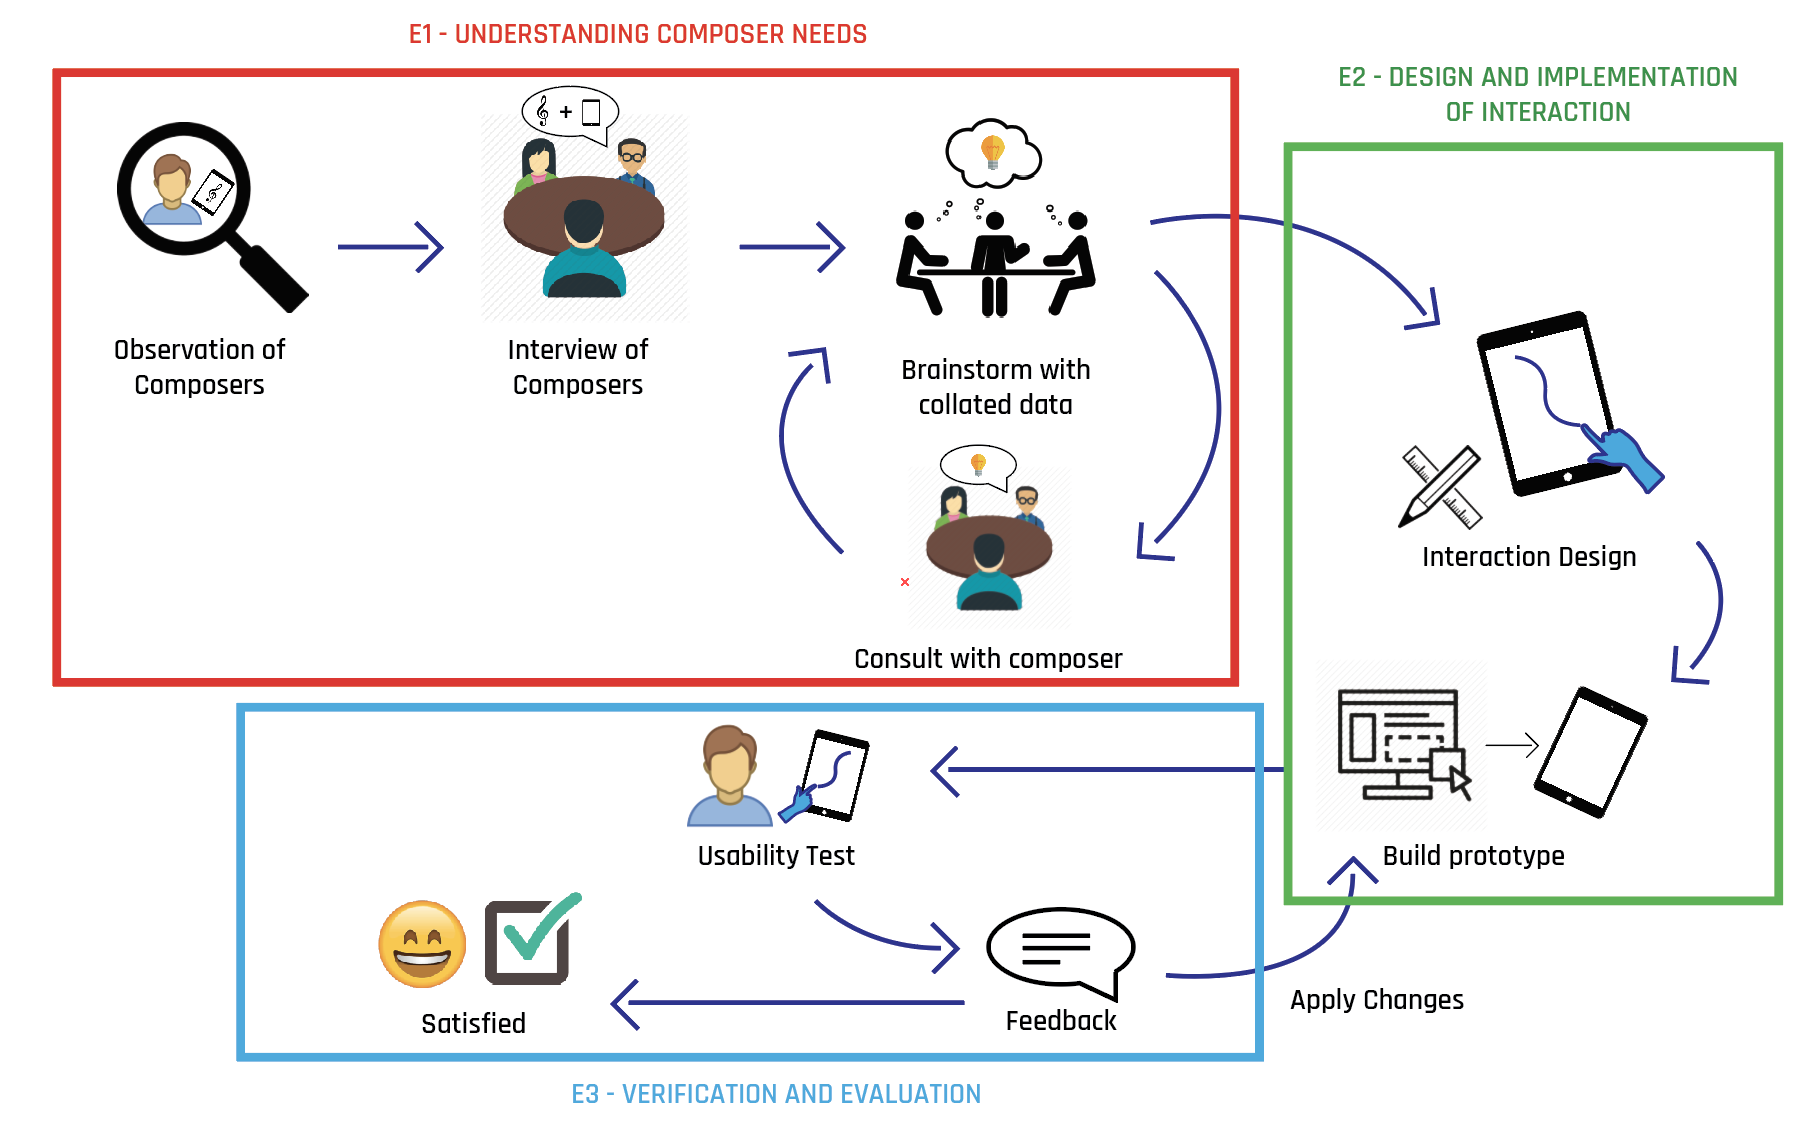
\includegraphics[scale=0.42]{figures/research_framework_sectioned.png}
	    \caption{The research framework for Flow.}
	    \label{fig:research_framework}
	\end{figure}

	The methodology for this study can be divided into three (3) main phases. The goal of the first phase (see Figure \ref{fig:research_framework} E1), is to understand the composers and identify their needs and problems. Using the gathered insights from the first phase, the second phase (see Figure \ref{fig:research_framework} E2)  will involve designing the interaction of the proposed solution. The last phase (see Figure \ref{fig:research_framework} E3) would then be an iterative process of testing and developing the proposed solution.


	\begin{comment}
	The goal of the first phase, \textit{understanding composer needs}, is to get to know more about the user and figure out their needs and pain points. User research and observation are key activities in this phase and is followed by interviews with composers to confirm and process the information as well as gather more insights. The points that were given by the composers would then be used in the brainstorming phase to determine a suitable solution. Consultations with composers will then be done to gather their insights on the proposed solution. This process will be repeated until the team is satisfied with the proposed solution.

	The next phase, \textit{design and implementation of interaction}, 
	\end{comment}

	\begin{comment}
	This study was designed to be repetitive and iterative, to allow for continuous improvement of the system. User research and observation are important steps to understanding the behavior of users and figuring out their pain points. This is followed by interviews with composers to confirm and process the information gathered from user tests and interviews. The points that were given by the composers would then be used in the brainstorming phase to determine a suitable solution. The team will then consult with the researchers about the proposed solution to gather their insights about it. The brainstorming would then be repeated to improve on the solution followed by another consultation. This would be repeated until the team is satisfied with the solution.

	The next phase would involve designing the interaction of the proposed solution. This would be followed by the prototype phase where a prototype would be built, tested, and improved repeatedly. Usability tests would be performed with different prototypes to create a good user experience. This phase would be repeated multiple times until the researchers are satisfied with the results of the tests.
	\end{comment}

	\begin{comment}
		Why/goal of the activity
		How we did it
	\end{comment}

	\section{Observation of Composers}

		Observations of the composers while they are composing music are necessary to understand the underlying thoughts and processes behind it. By doing this, the researchers should be able to understand the thought-process and actions that composers undergo when composing music. The goal of this activity is to gather initial findings on the needs or pain points that the composers might have while composing. 

		This activity will mainly be done in the studio of the composers or any place where they normally compose. The presence of instruments or any other tools will depend on the composer as long as it simulates their natural composition process. 


	\section{Interview of Composers}

		Interviews will be done to confirm and process the information and insights gathered from the observations made in the previous activity. Aside from this, further questions will be asked about their process of musical composition, the tools, and the techniques they use. The main purpose of this activity is to get further context on the composition process and identify aspects that might not have been covered by the observations. 

		The main questions to be asked in the interview are: 
		\begin{enumerate}
			\item What is your process of musical composition? What do you usually do?
			\item What techniques do you use during musical composition?
			\item What tools do you use when composing?
			\item What features do you like or often use in the tools you use?
			\item What are the difficulties you encounter when composing music? 
		\end{enumerate}

		Note that these are only the main questions and not all of the questions. Different questions may come up depending on how the composer would answer a question to gather more insights. 

	\section{Brainstorm with Collated Data}

		After the observations and interviews, it is necessary to filter and process the gathered data to identify the needs and pain points of the target users. These needs and problems would then be the main focus when thinking of proposed solutions. 

		This study will employ an affinity diagram for brainstorming. The affinity diagram is simply a tool that groups data or findings based on their relationships. This is done by identifying key points, observations, or ideas from composers that stand out and writing them on sticky notes. These may be behaviors, activities, things they said, or problems they encountered while composing and the workarounds they did to fix the problem. After writing them out, the items are grouped based on their relationships to identify similar or recurring ideas or problems. The affinity diagram will help identify the problem statement to focus on.

		With the problem statement in mind, the researchers can then ideate possible solutions. Ideation sessions put no limit on the amount of ideas that were generated; the more ideas the better. The researchers will then vote on the ideas they like and also provide suggestions on how to improve it. 

	\section{Consult with Composer}

		When a possible solution is thought of in the brainstorming activity, this will then be consulted with the composers, the people who would actually use the it. Feedback and suggestions will also be gathered to help improve the proposed solution solution. This, along with the previous activity, will be repeated until both the composers and researchers are satisfied.

		\subsection{System Features}

			From the feedback and insights gathered from the interviews and brainstorming sessions, it was found that the application should at least have the following features: 
			\begin{itemize}
    			\item View, create, edit, and delete their own compositions
    			\item Set the key and time signature of their compositions
    			\item Highlight/select a note or a group of notes
             	\item Add, edit, and delete notes/rests 
              	\item Add, edit, and delete polyphonic notes (chords)
           		\item Transpose a note or group of notes
        		\item Add ties/slurs to notes
              	\item Add, remove, or change an accidental on a note or group of notes
              	\item Add or remove dots on a note or group of notes
              	\item Apply retrograde/inversion on a note or group of notes
              	\item Cut, copy, and paste a note/rest or a group of notes/rests
              	\item Undo/redo an action
              	\item Zoom in our zoom out of the interface
              	\item Change the tempo
              	\item Listen to or play their composition
          	\end{itemize}				

	\section{Interaction Design}





	\section{Build Prototype}

		The initial, mid-fidelity prototype was built using InVision, a prototyping tool. Note that this was nowhere near an actual application and only consisted of screenshots or ``screens'' where users can interact with using the limited gestures in InVision. Despite the limited interactions available, doing this was quicker than actually developing the application, making it better for the earlier stages of testing the interaction design. The mid-fidelity prototype allowed the researchers to test out initial interaction design decisions and easily make the necessary changes. 

		Once the initial interaction design became clearer and more defined, it needed to be tested on a better platform since InVision was only limited to images and could never capture the complete interaction of the actual application. A high-fidelity prototype was then built for iOS and the iPad using Swift 4. This prototype went through four (4) versions, having changes in the interaction and the user interface. 

	\section{Usability Test}

		The objective of the tests will be to determine if the interaction and design of the system augments the user experience of the composer when interacting with the application, Flow. The researchers will be collecting quantitative and qualitative data. The quantitative data will mainly come from a survey  about the usability of the features that the testers will have to answer. The qualitative data will come from the video and audio recording of the testers as well as the interviews done after the tests. The functionality will also be closely monitored to see if there are glitches or bugs that require additional fixes in the development side. These bugs or glitches will warrant an intervention from the researchers during the testing. 

		The tests will be conducted in an environment where audio and visual disturbances are at a minimum. This is to ensure that the researchers are able to analyze clear audio and video data from the recording devices used during the testing. This is also to ensure that the tester is not disturbed during the testing. 

		%The setups used across all the user tests are 4 kinds of Flow system prototypes, 1 created using a prototyping tool called InVision, and 3 coded in Swift; 2 kinds of commercially available notation applications in the App Store, Notion and Komp; and the traditional form of composition which is using music sheets and writing materials. Notation softwares and the Flow prototypes will be launched on a mobile platform, namely an IPad tablet.

		Before starting the test, testers will be given a consent form. If they agree with the terms and continue with the testing, the tasks indicated in Section \ref{sec:tasks} will be done for each test setup (indicated in Section \ref{sec:test-setups}) that is appropriate. Before the start of the test where the tester start to accomplish tasks or use cases for the test setup, they will be given a brief description of the objectives of the study along with overview of the tasks or use cases. 

		During the first two (2) iterations, five (5) subjects of both genders aged 18-40 were recruited through snowball sampling method to take part in the data collection and testing. These subjects were categorized into two (2) user groups based on musical composition experience: amateur, and experienced. For the third iteration, fifteen (15) subjects of the same demographics took part in the testing. In the last iteration, eleven (11) subjects took part. 

		% TODO describe demographics

		\subsection{Test Setups}
		\label{sec:test-setups}

			The setups between the preliminary testing and the subsequent testing were different. This was made so because the main goal of the preliminary testing was to gather feedback on the interaction design and help improve the system while it was still being developed. Other applications did not matter as much and were only used to gain insight on their interactions and how they could be used to improve the system. Although the goal of the subsequent tests were still to gather feedback and improve the system, they were also made to compare the system against similar musical composition applications. 

			\subsubsection{Preliminary Testing Setups}

				The test setups are meant to observe how existing methods of composition work and how their interactions could be used in Flow. The tasks enumerated in Section \ref{sec:preliminary-tasks} will be used in each test setup whenever possible since some tasks can only be accomplished within a specific setup. 

				There will be 3 different test setups to be used during user testing namely:

				\begin{itemize}
					\item Tester composing using music sheets
					\item Tester composing using Komp
					\item Tester composing using Flow
				\end{itemize}

				The first setup simulates the traditional way of musical composition. This is through music sheets and a writing instrument. Traditional music sheets will be provided by the researchers as well as a choice of using a pen or pencil for writing musical elements. The composers are free to use as much music sheets as they want for drafting and experimenting with their composition as long as the time and resources provided by the researchers allow them.

				The second setup will be through an existing mobile application for iOS platforms, komp. Since the method of input in komp is similar to writing in music sheets, this setup will mainly be done to see how the interaction for traditional musical composition will work when applied to mobile devices. The researchers expect this setup to have similar results with the first setup and any data collected in this setup will be used to evaluate Flow.

				The third setup will be focused on the composer using the developed system, Flow. During the early periods of testing, a mid-fidelity InVision prototype will be used as a substitute. Using this prototype, the only task that the composer will be able to do is to explore the application. The main goal of this is to develop and improve the interaction design of the application. One a high-fidelity prototype has been developed, all tasks will be performed in the testing.

			\subsubsection{Subsequent Testing Setups}

				In the subsequent tests, Flow was compared against other musical notation applications. For each setup, the users had to go through the use cases listed in \ref{sec:use-cases} and perform the tasks outlined in \ref{sec:subsequent-tasks}. Note that these setups were given in random order and that the application developed by the researchers was not disclosed to prevent bias.

				\begin{itemize}
					\item Tester composing using Notion
					\item Tester composing using komp
					\item Tester composing using Flow
				\end{itemize}

				The first setup makes use of what is said to be the most popular musical notation application for mobile. For the second setup, komp is retained from the preliminary testing so that users can experience a traditional method of notation while on the iPad. The last setup makes use of the system developed by the researchers.

			\subsubsection{Use Cases}
			\label{sec:use-cases}

				For the subsequent test setups, the testers had to go perform use cases. These use cases were an attempt to simulate different musical composition scenarios. 

				\begin{itemize}
				    \item Compose a familiar song (Twinkle Twinkle Little Star/Happy Birthday)
				    \item Compose from scratch
				    \item Modify a composition (Ode to Joy/Amazing Grace)
				\end{itemize}

		\subsection{Tasks}
		\label{sec:tasks}

			Similar to the test setups, the tasks differed greatly between the preliminary testing and subsequent testing. Tasks were generalized in the subsequent testing to make it easier for the testers to compare the different applications.

			\subsubsection{Preliminary Testing Tasks}
			\label{sec:preliminary-tasks}

				Some tasks may be omitted in different test setups when a crucial function to carry out the task is unavailable. During the final task, testers are encouraged to speak aloud their concerns and opinions regarding the application.

				For the first iteration, there will be 4 tasks for each of the setups:
				\begin{itemize}
					\item Add a note
					\item Add a series of notes
					\item Change a note
					\item Delete/remove a series of Notes
					\item Compose for 3 minutes
				\end{itemize}

				For the second iteration, there will be 7 tasks for each of the setups:
				\begin{outline}
					\1 Add notes to fill 2 measures
					\1 Change the time signature to 3/4
					\1 Empty one measure
					\1 Empty the composition
					\1 Add enough notes to fill 2 measures in 2 staffs
					\1 Add an accidental to 2 notes
					\1 Remove placed accidentals 
					\1 Change key signature
					\1 Replace a group of notes with a single note
					\1 Create or recreate a composition (Exactly 4 measures)
						\2 Twinkle Twinkle Little Star
						\2 Canon in D
						\2 Ode to Joy
				\end{outline}

			\subsubsection{Subsequent Testing Tasks}
			\label{sec:subsequent-tasks}

				Since one of the goals of the subsequent tests was to compare how the interaction was against similar applications, the tasks were greatly simplified and generalized. Testers were also allowed to perform the tasks in any order they wanted and as much repititions it took for them to get acquainted with the specific task or action. These tasks were repeated for each of the use cases mentioned in \ref{sec:use-cases}.

				\begin{itemize}
					\item Select/highlight notes/chords
				  	\item Add notes/chords
				  	\item Edit notes/chords
				  	\item Delete notes/chords
				  	\item Cut, copy, or paste notes/chords
				  	\item Undo/redo an action
				  	\item Play the composition
				\end{itemize}


	\section{Feedback}

\begin{comment}
% \section{System Architecture and Framework}
\section{System Description}

\subsection{System Overview}

The system will integrate music theory and user experience in an interface for musical composition. The composition process of composers will be observed and analyzed so that the system can be built to fit this process. The system will undergo multiple revisions based on the results of user testing. It will be built for the iOS, but will be optimized for the iPad. It will provide users an interface to create/edit, and view compositions. The user can make use of the system through an interface containing compositional activities like adding, editing, and deleting notes. Finally, the system will allow users to save their composition, which can be imported to a MusicXML format.

\subsection{System Objectives}

	\subsubsection{General Objective}
		
        To provide an interface that allows composers to perform basic and advanced musical composition tasks via gesture interactions on a mobile platform.

	\subsubsection{System Features}
    
    	Specifically, the system will allow users to do the following: 
    		\begin{enumerate}
    			\item View, create, edit, and delete their own compositions
    			\item Set the key and time signature of their compositions
    			\item Highlight/select a note or a group of notes
             	\item Add, edit, and delete notes/rests 
              	\item Add, edit, and delete polyphonic notes (chords)
           		\item Transpose a note or group of notes
        		\item Add ties/slurs to notes
              	\item Add, remove, or change an accidental on a note or group of notes
              	\item Add or remove dots on a note or group of notes
              	\item Apply retrograde/inversion on a note or group of notes
              	\item Cut, copy, and paste a note/rest or a group of notes/rests
              	\item Undo/redo an action
              	\item Zoom in our zoom out of the interface
              	\item Change the tempo
              	\item Listen to or play their composition
          \end{enumerate}
    
\subsection{Scope and Limitations of the System}

Given that the system is on a mobile platform, it would be limited in ability compared to that of desktop applications. This system aims to be a sketching application for composers that are on the go, or do not have their computers available. It will not contend with full-blown desktop musical composition applications like Finale or Sibelius.

Musical composition can be done for several kinds of instruments. However, the way music is composed varies from one instrument to another. With that said, the system will only support compositions for the piano. The system will also limit the musical notation symbols that can be used. The ones available for use are: 

\begin{itemize}
	\item Sixty-fourth note to whole note
    \item Sixty-fourth rest to whole rest
    \item Accidentals (sharp, flat, double-sharp)
\end{itemize}

Composers will also need to save their compositions in cases where they could not finish entirely and want to go back to it. A composition also has several elements which would be hard to model in databases. Thus, MusicXML will be used as the file format for saving data. This also makes it easy to transfer work from the system to other musical composition applications.

Gesture interactions are the main method of interaction within the system. Some gestures like tapping on the line need to be accurate and precise. To improve this precision, bigger screens will be needed. The iPad will be the best for this due to it having a large screen, yet still being portable. The testing will also be done on the iPad only.

Finally, the system's potential musical metacreation feature will need to have a model for generating the succeeding notes. To make it lightweight, the system will make use of a rule-based model similar to that of Computoser \citep{bozhanov2014computoser} and SuperWillow \citep{schulze2011music}. The model will take into account music theory for its rules.

\subsection{Data Design}

Given that musical compositions have a lot of elements which need to be stored as data, using relational databases for storage would prove to be inefficient and unintuitive \citep{hristidis2003efficient}. That is why the system would represent data through the use of MusicXML, which was also used in the SuperWillow system found in the study of \citeauthor{schulze2011music}.

MusicXML is a method of storing and representing digital sheet music through XML \citep{makemusic2017musicxml}. Because it is an Extensible Markup Language (XML), it follows a specific format that defines a logical structure \citep{bray1997extensible}, which in this case is a musical composition. The advantage of the MusicXML format is that it is used in several musical composition applications and can easily be shared between these applications \citep{makemusic2017musicxml}. Also, it can represent the most complicated aspects of musical notation like repeats, slurs, and more.

Shown in Table \ref{tab:musicxml} are the some of the commonly used elements and their respective descriptions in MusicXML.
 
\begin{longtable}{|p{3.6cm}|p{10cm}|} 
\caption{Commonly Used MusicXML Elements} \label{tab:musicxml} \\
\hline
       
       Element & Description \\ \hline
		
        \texttt{<score-partwise>} & Defines that the composition is divided into several parts, and these parts can have multiple measures. \\ \hline
        
        \texttt{<score-timewise>} & An alternative to the \texttt{<score-timewise>}, it defines the composition to have multiple measures where the measures can have many parts. \\ \hline

		\texttt{<part-list>} & Lists the parts of the composition. \\ \hline
        
        \texttt{<score-part>} & To be used as a child of \texttt{<part-list>}, this element adds a new part to the composition. Commonly supplied with the \texttt{id} attribute. \\ \hline
        
        \texttt{<part-name>} & A child of the \texttt{<score-part>} element, specifies the name of its parent part. \\ \hline
        
        \texttt{<attributes>} & Lists essential information in the composition such as the key, time signature, and clef. \\ \hline
        
        \texttt{<divisions>} &  Used in the production of sound. It works with the \texttt{<duration>} element to tell how many divisions per quarter note equal to the duration indicated. \\ \hline
        
        \texttt{<key>} & Denotes which key signature the composition is in and contains the \texttt{<fifths>} element. \\ \hline
        
        \texttt{<fifths>} & This element is derived from the circle of fifths and says how many sharps or flats the composition has. \\ \hline
        
        \texttt{<time>} & The time element contains information about the time signature which can be set using the \texttt{<beats>} and \texttt{<beat-type>} tags. \\ \hline
        
        \texttt{<beats>} & The numerator of the time signature. \\ \hline
        
        \texttt{<beat-type>} & The denominator of the time signature. \\ \hline
        
        \texttt{<clef>} & Tells the clef to be used in the composition through the \texttt{<sign>} and \texttt{<line>} tags. \\ \hline
        
        \texttt{<sign>} & Specifies the sign to be used for the clef.\\ \hline
        
        \texttt{<line>} & Specifies which line the set sign will start. \\ \hline
        
        \texttt{<note>} & Contains information inside that is needed to define a single note. \\ \hline
        
        \texttt{<pitch>} & Located inside the \texttt{<note>} element, it contains the \texttt{<step>} and \texttt{<octave>} elements that would indicate where the note would be placed. \\ \hline
        
        \texttt{<step>} & Indicates the pitch step. Must always be supplied in the \texttt{<pitch>} element. \\ \hline
        
        \texttt{<octave>} & Indicates the octave of the pitch. Also required. \\ \hline

        \texttt{<alter>} & An optional element in the \texttt{<pitch>} that indicates if the note has a sharp or flat. \\ \hline
        
        \texttt{<duration>} & Also an element inside the \texttt{<note>}, it works with the \texttt{<division>} element to denote what kind of note or sound it would play. \\ \hline
        
        \texttt{<type>} & Mainly serves to indicate how the note will be displayed or notated. \\ \hline


\end{longtable}

Whenever a user creates a composition and saves it in the application, a corresponding MusicXML will be generated and saved in the device's local storage. The MusicXML will be used to load the composition again, in case the user wants to edit or view it. 

\subsection{System Framework}

\begin{figure}[H]
	\centering
	
\includegraphics[scale=0.4]{System_Framework}
    \caption{The system framework for Flow.}
    \label{fig:systemframework}
\end{figure}

The system framework, shown in Figure \ref{fig:systemframework}, illustrates an overview of how Flow works. Input is relatively simple, mainly in the form of gestures. Users can tap, swipe, hold, or drag on specific objects. The application's gesture recognizer would then analyze the gesture performed by the user. The system would then output or perform the specific action assigned to each gesture. However, if the gesture is tied to musical metacreation, the application would output a set of notes based on its built-in algorithm.

\subsection{System Walkthrough}

\subsubsection{Main Menu}
The Main Menu (Figure \ref{fig:main-menu}) is the first screen shown to the user upon opening the application. This screen is where the user can create, open, export, and delete a composition. 

\subsubsection{Creating a Composition}
To create a new composition, the user may tap on the '+' icon which will lead to the Editor screen. 

\begin{figure}[H]
	\centering
	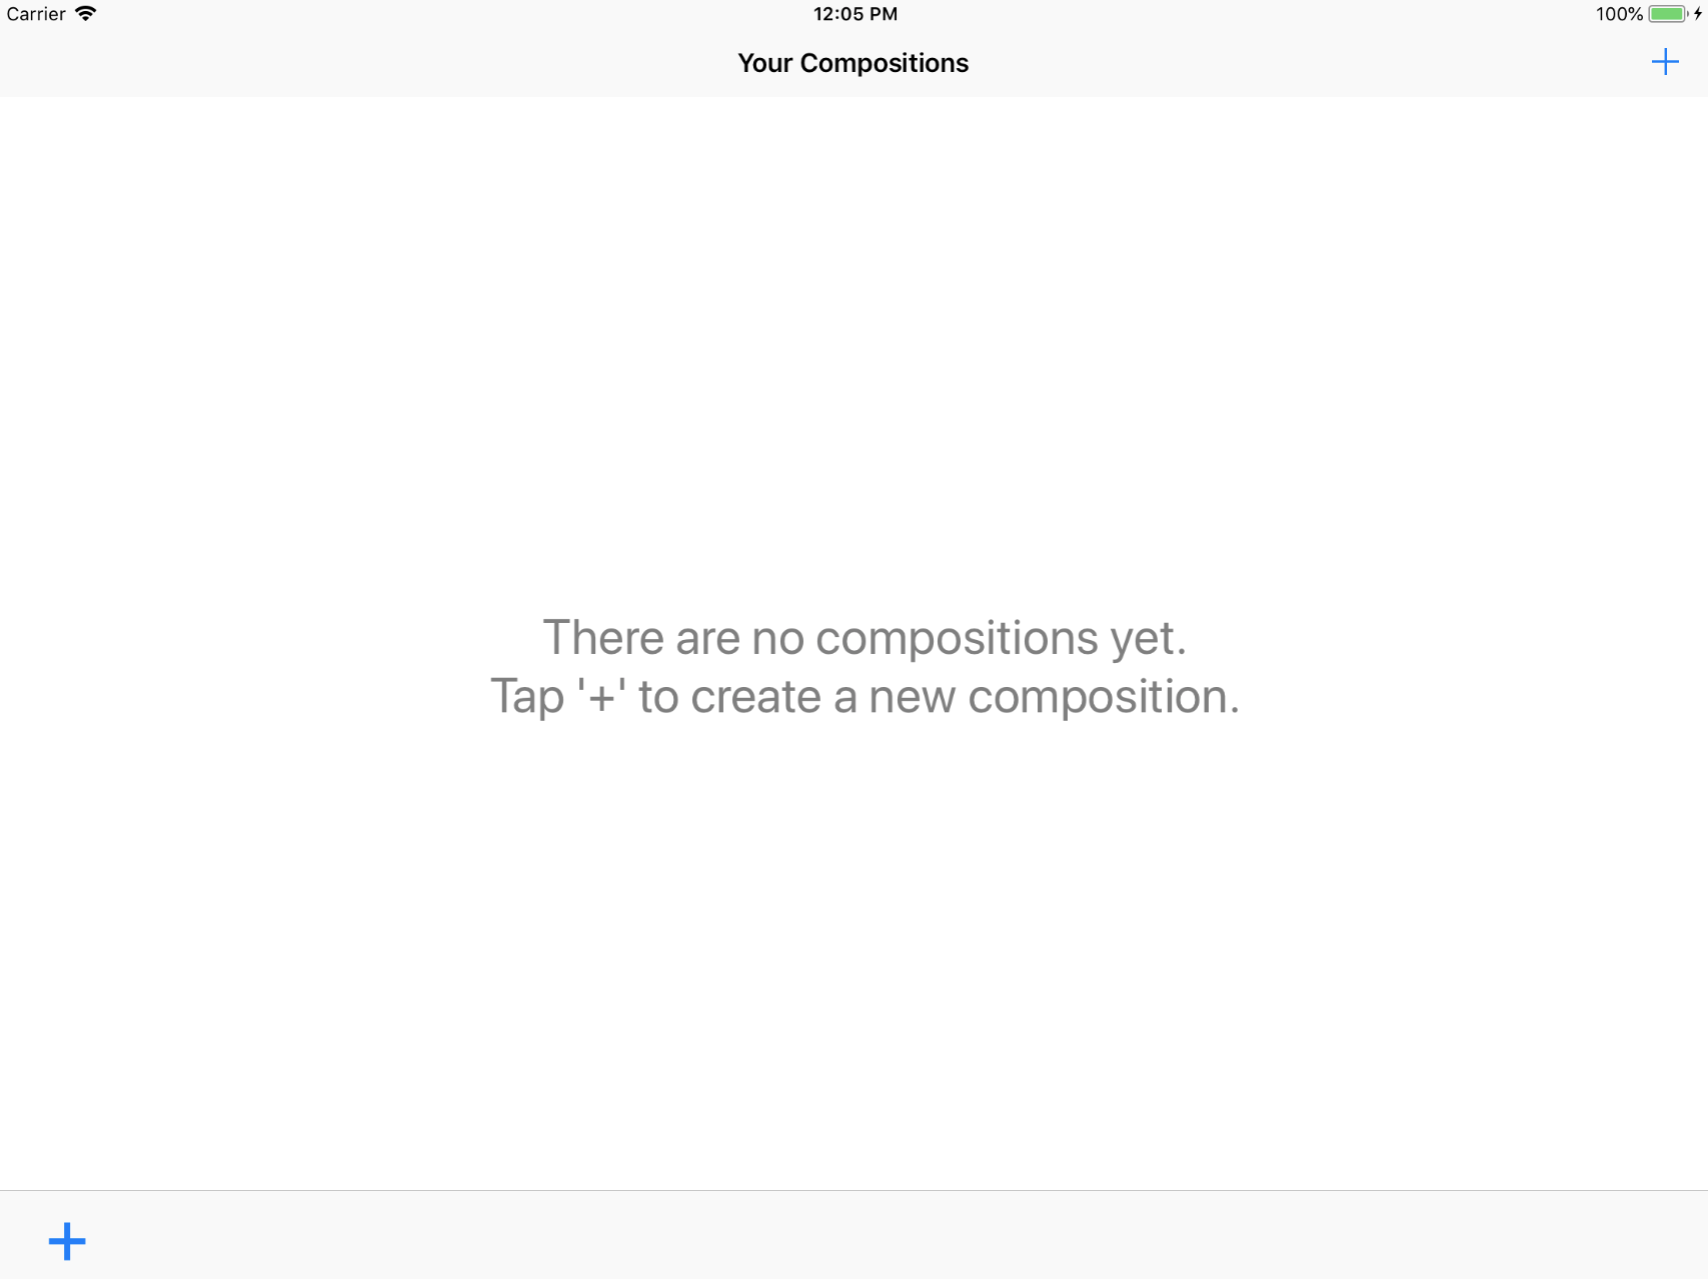
\includegraphics[scale=0.4]{Main_Menu}
    \caption{Flow Main Menu.}
    \label{fig:main-menu}
\end{figure}

\subsubsection{Opening a Composition}
Tapping an existing composition in the list will open it in the Editor screen allowing the user to edit. 

\subsubsection{Deleting, Renaming, and Exporting a Composition}
Swiping a composition to the left brings out the delete button (Figure \ref{fig:swipe-delete}). The user may also tap and hold an existing composition which brings out a modal for exporting (share), renaming, and deleting a composition (Figure \ref{fig:tap-hold-comp}).

\begin{figure}[H]
	\centering
	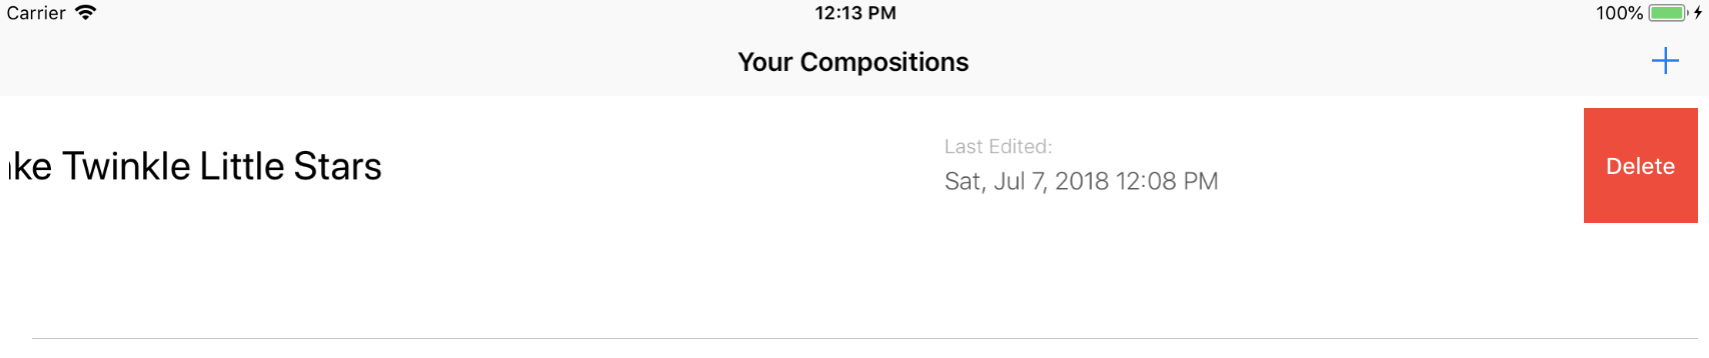
\includegraphics[scale=0.45]{Swipe_Delete}
    \caption{Swipe left to delete a composition.}
    \label{fig:swipe-delete}
\end{figure}

\begin{figure}[H]
	\centering
	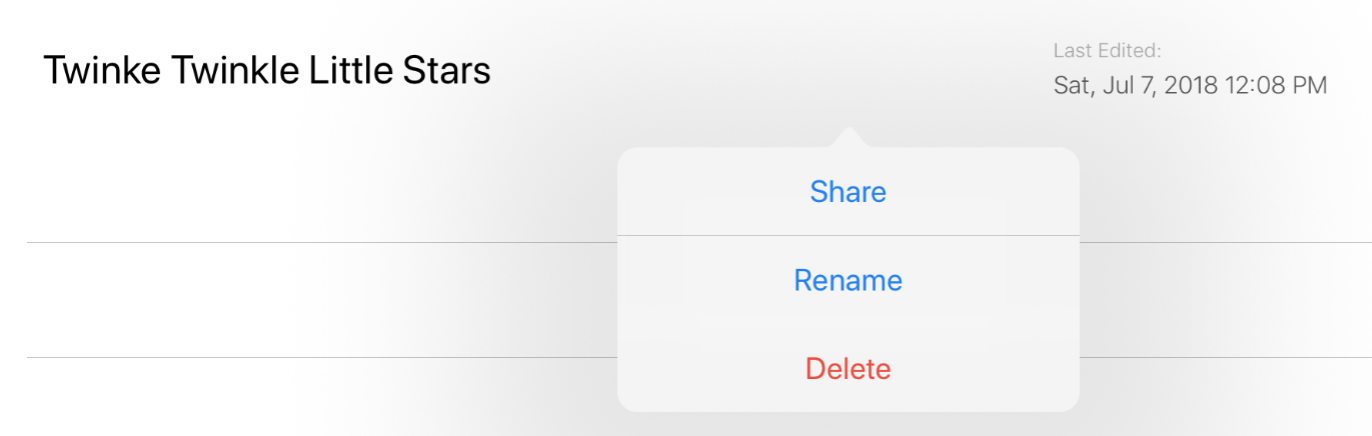
\includegraphics[scale=0.45]{Tap_And_Hold_Comp}
    \caption{Tap and hold a composition to bring out modal.}
    \label{fig:tap-hold-comp}
\end{figure}

\subsubsection{Editor}

The editor screen is where the user will spend most of the time using the application. It is where most of the composition process will take place. This includes adding, editing, and deleting of notes, rests and accidentals, setting the title, key signature, time signature, and tempo of the composition. This is also where the user can listen to the current progress of a composition through the playback functionality and also save a composition. Shown in Figure \ref{fig:editor} is the editor screen after creating a new composition from the main menu. 

\begin{figure}[H]
	\centering
	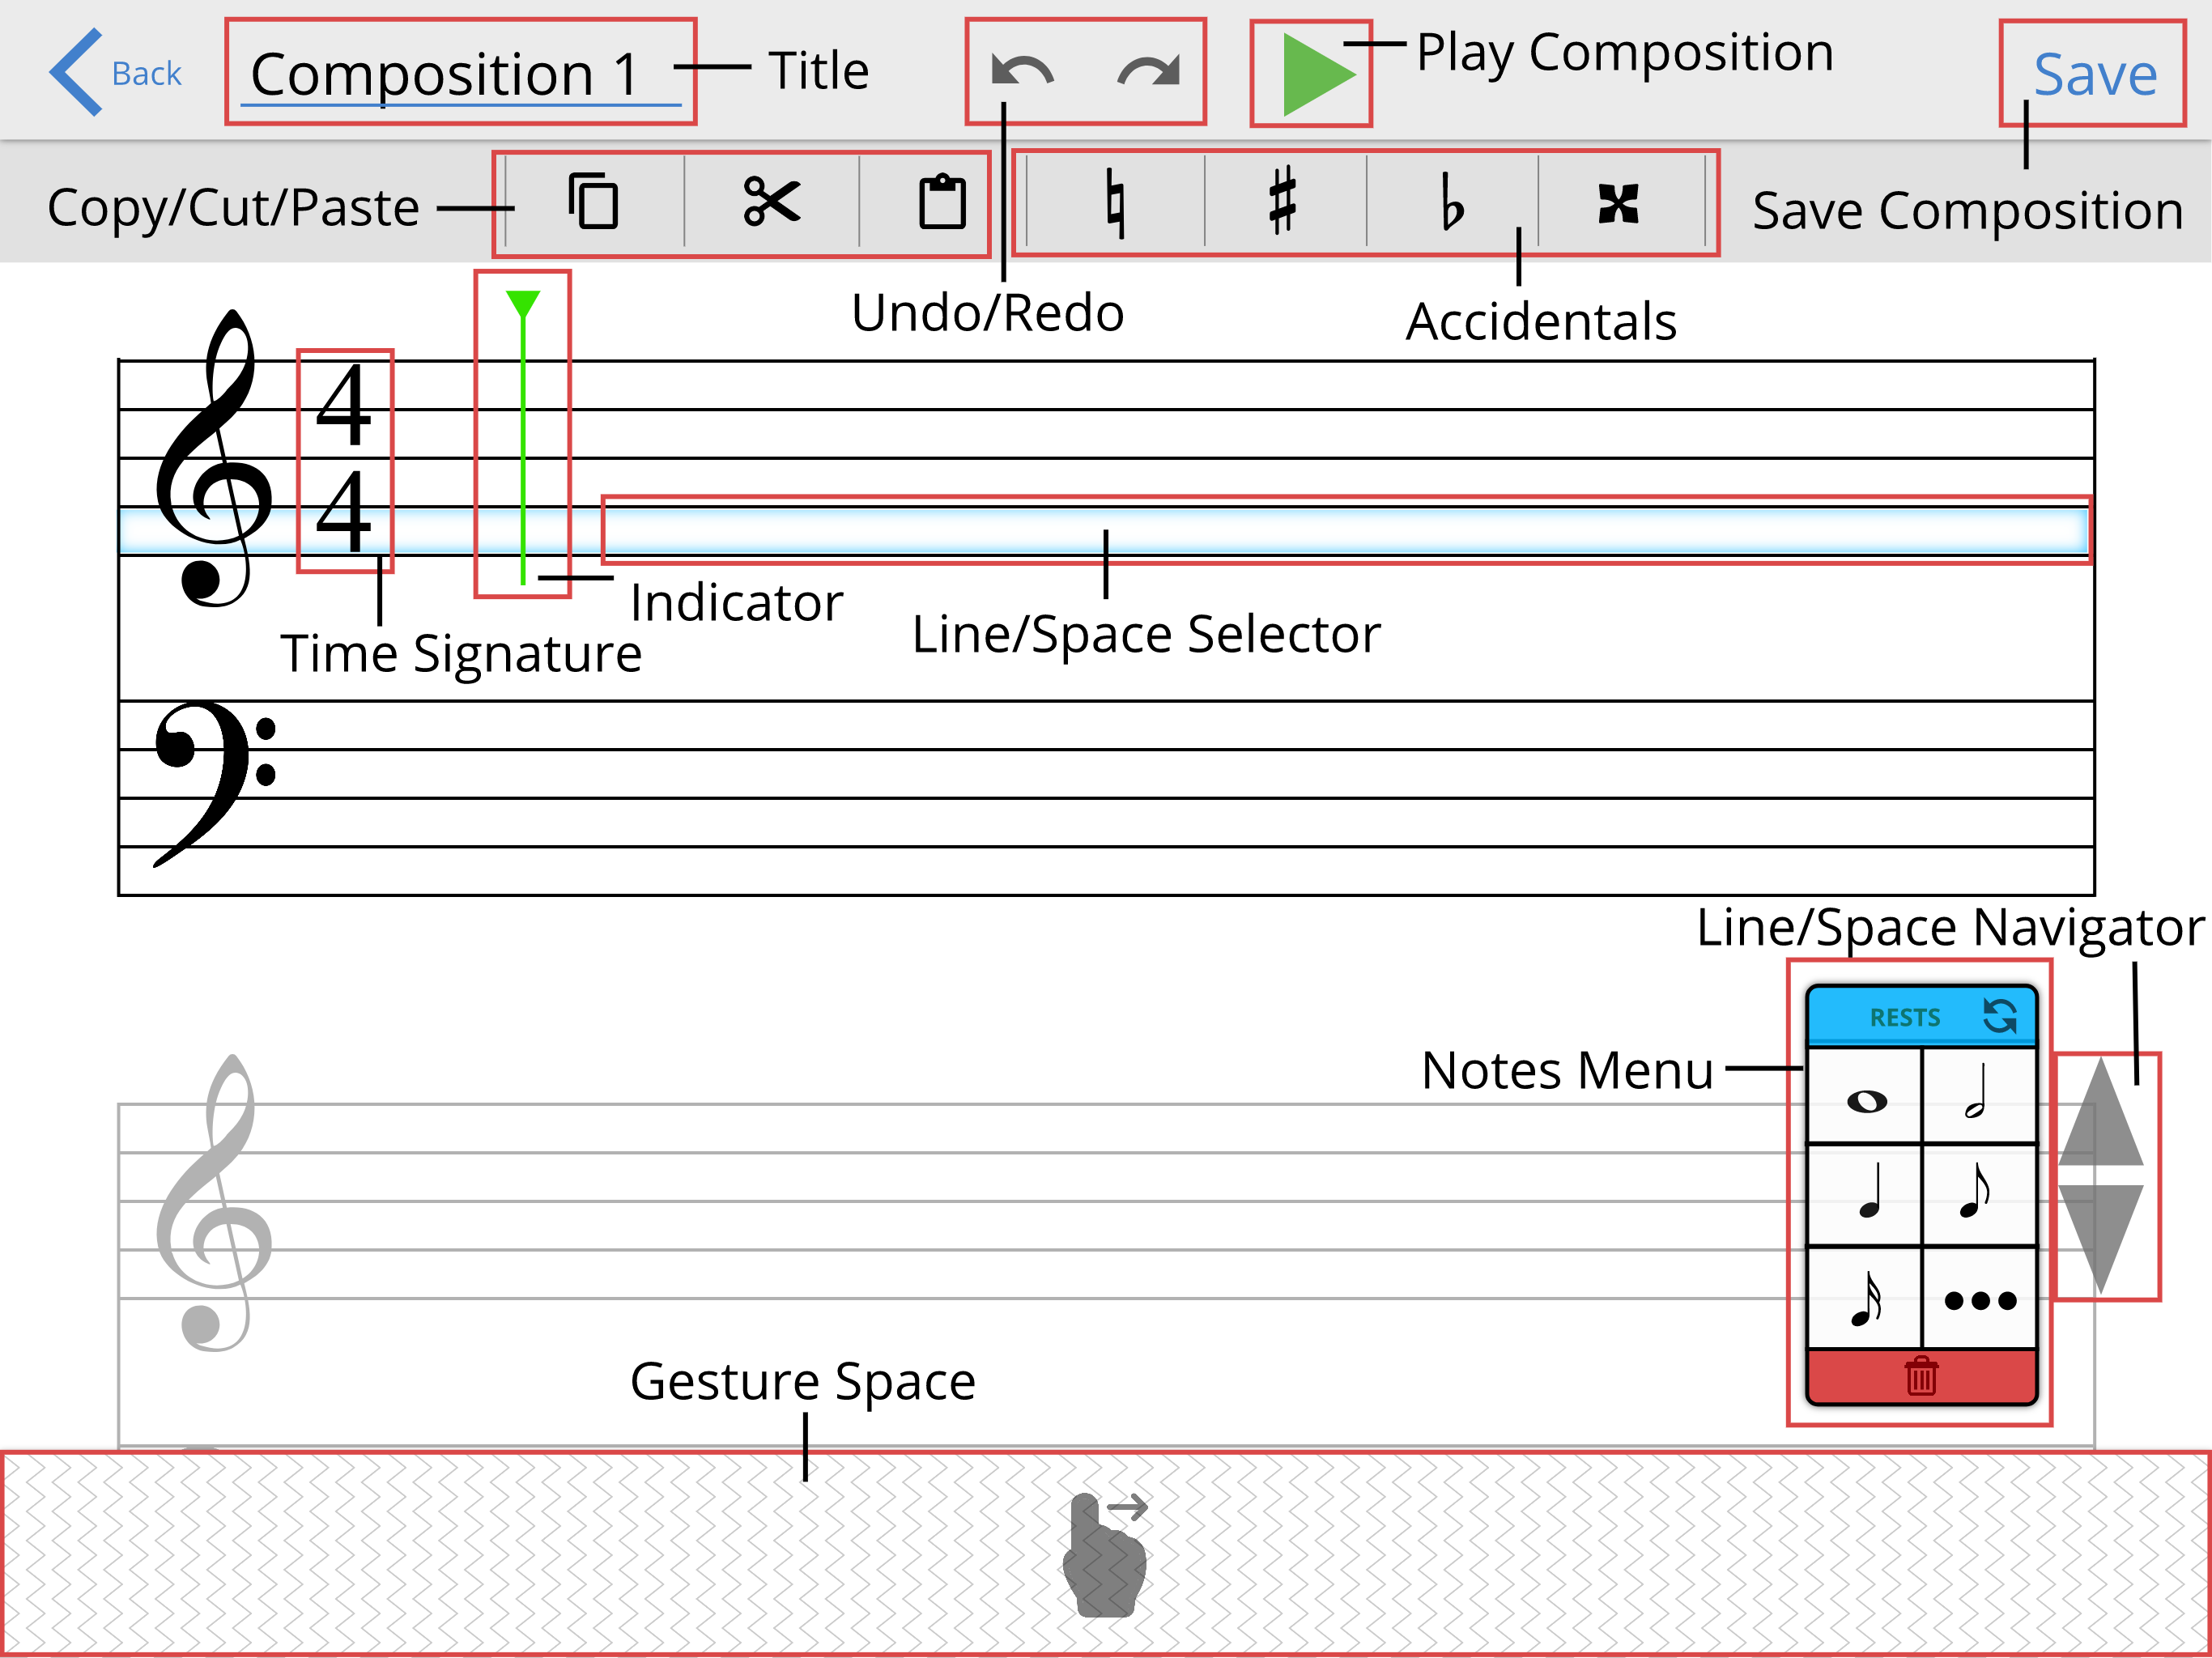
\includegraphics[scale=0.45]{Editor}
    \caption{Editor Screen.}
    \label{fig:editor}
\end{figure}

\subsubsection{Zooming and Panning}
To zoom out on the editor, the user must use the pinch in gesture (Figure \ref{fig:pinch-in}) and to zoom in, the user must use the pinch out gesture (Figure \ref{fig:pinch-out}). To pan the editor, the user must do a 2 finger drag gesture.

\begin{figure}[H]
	\centering
	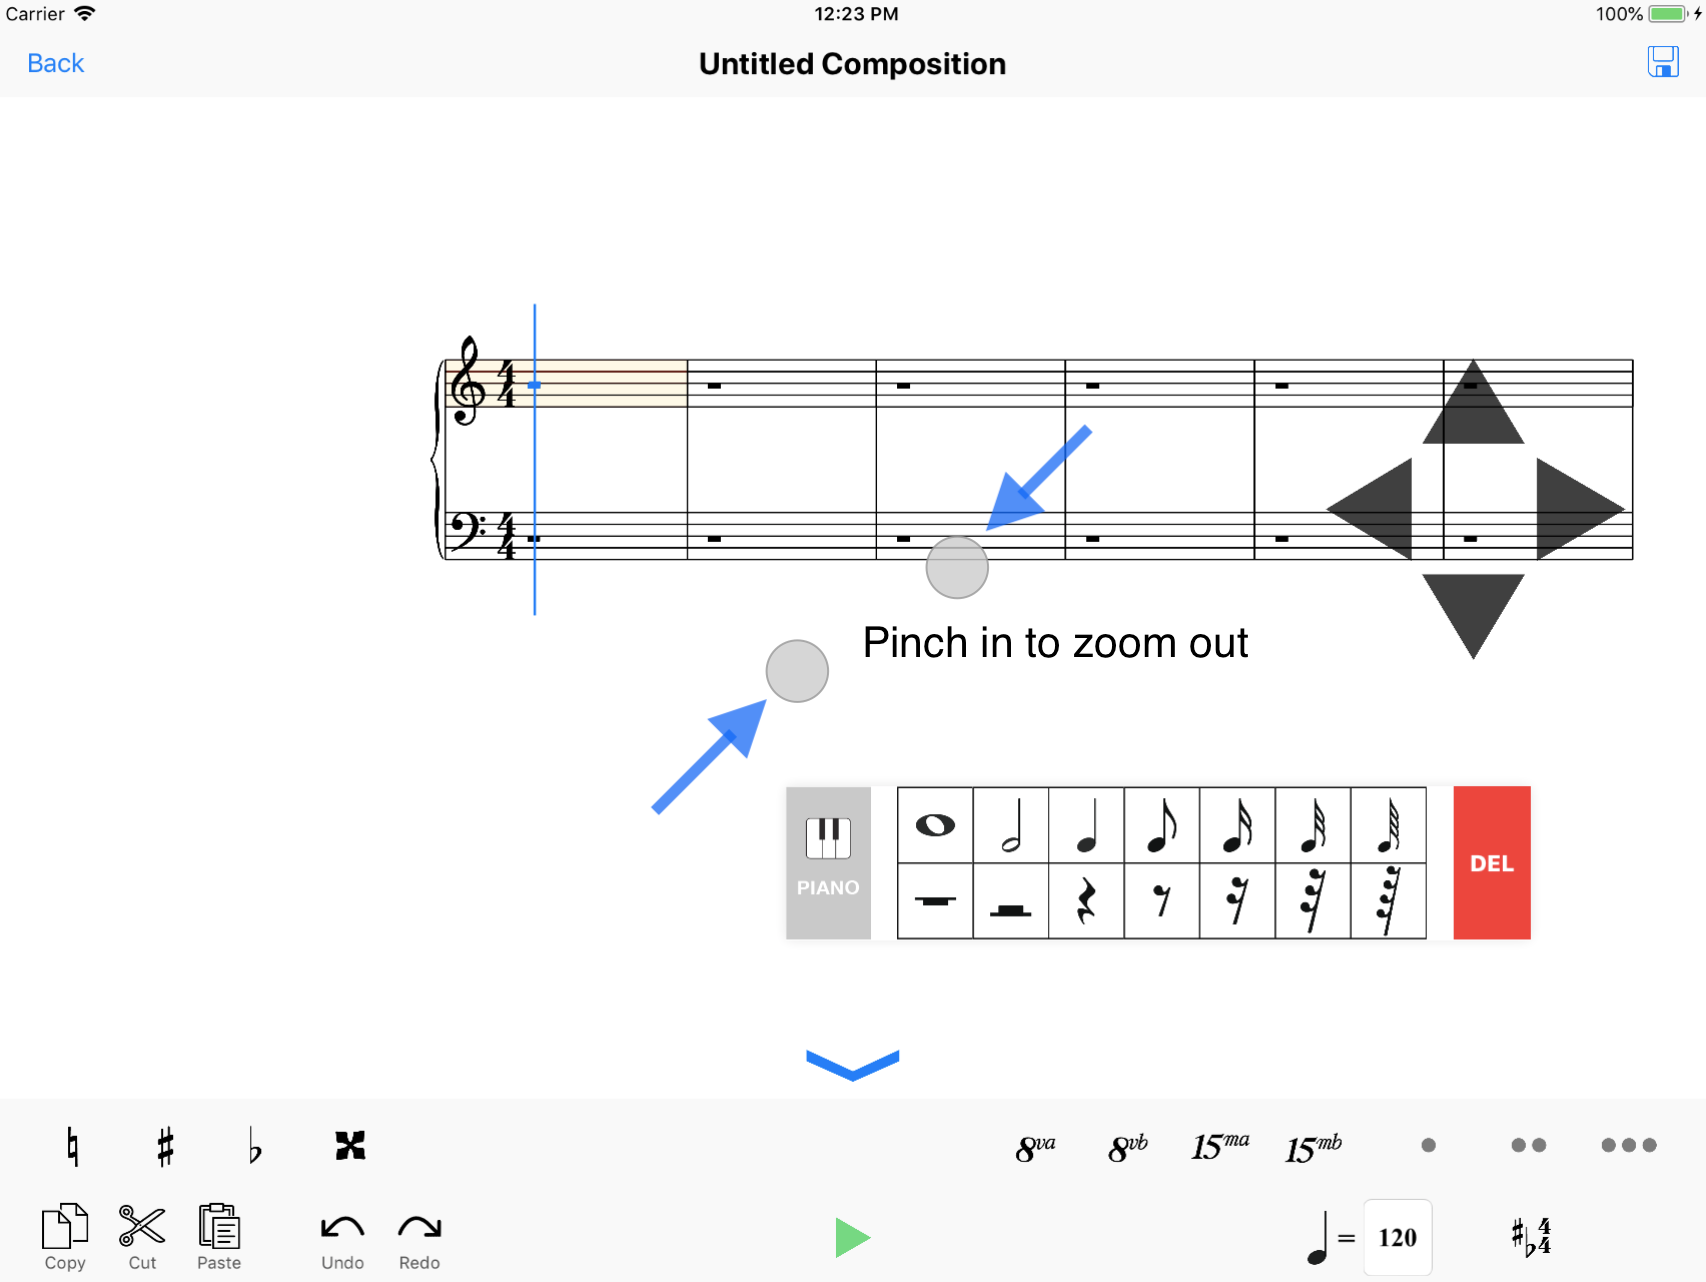
\includegraphics[scale=0.4]{Pinch_In}
    \caption{Pinch in to zoom out.}
    \label{fig:pinch-in}
\end{figure}

\begin{figure}[H]
	\centering
	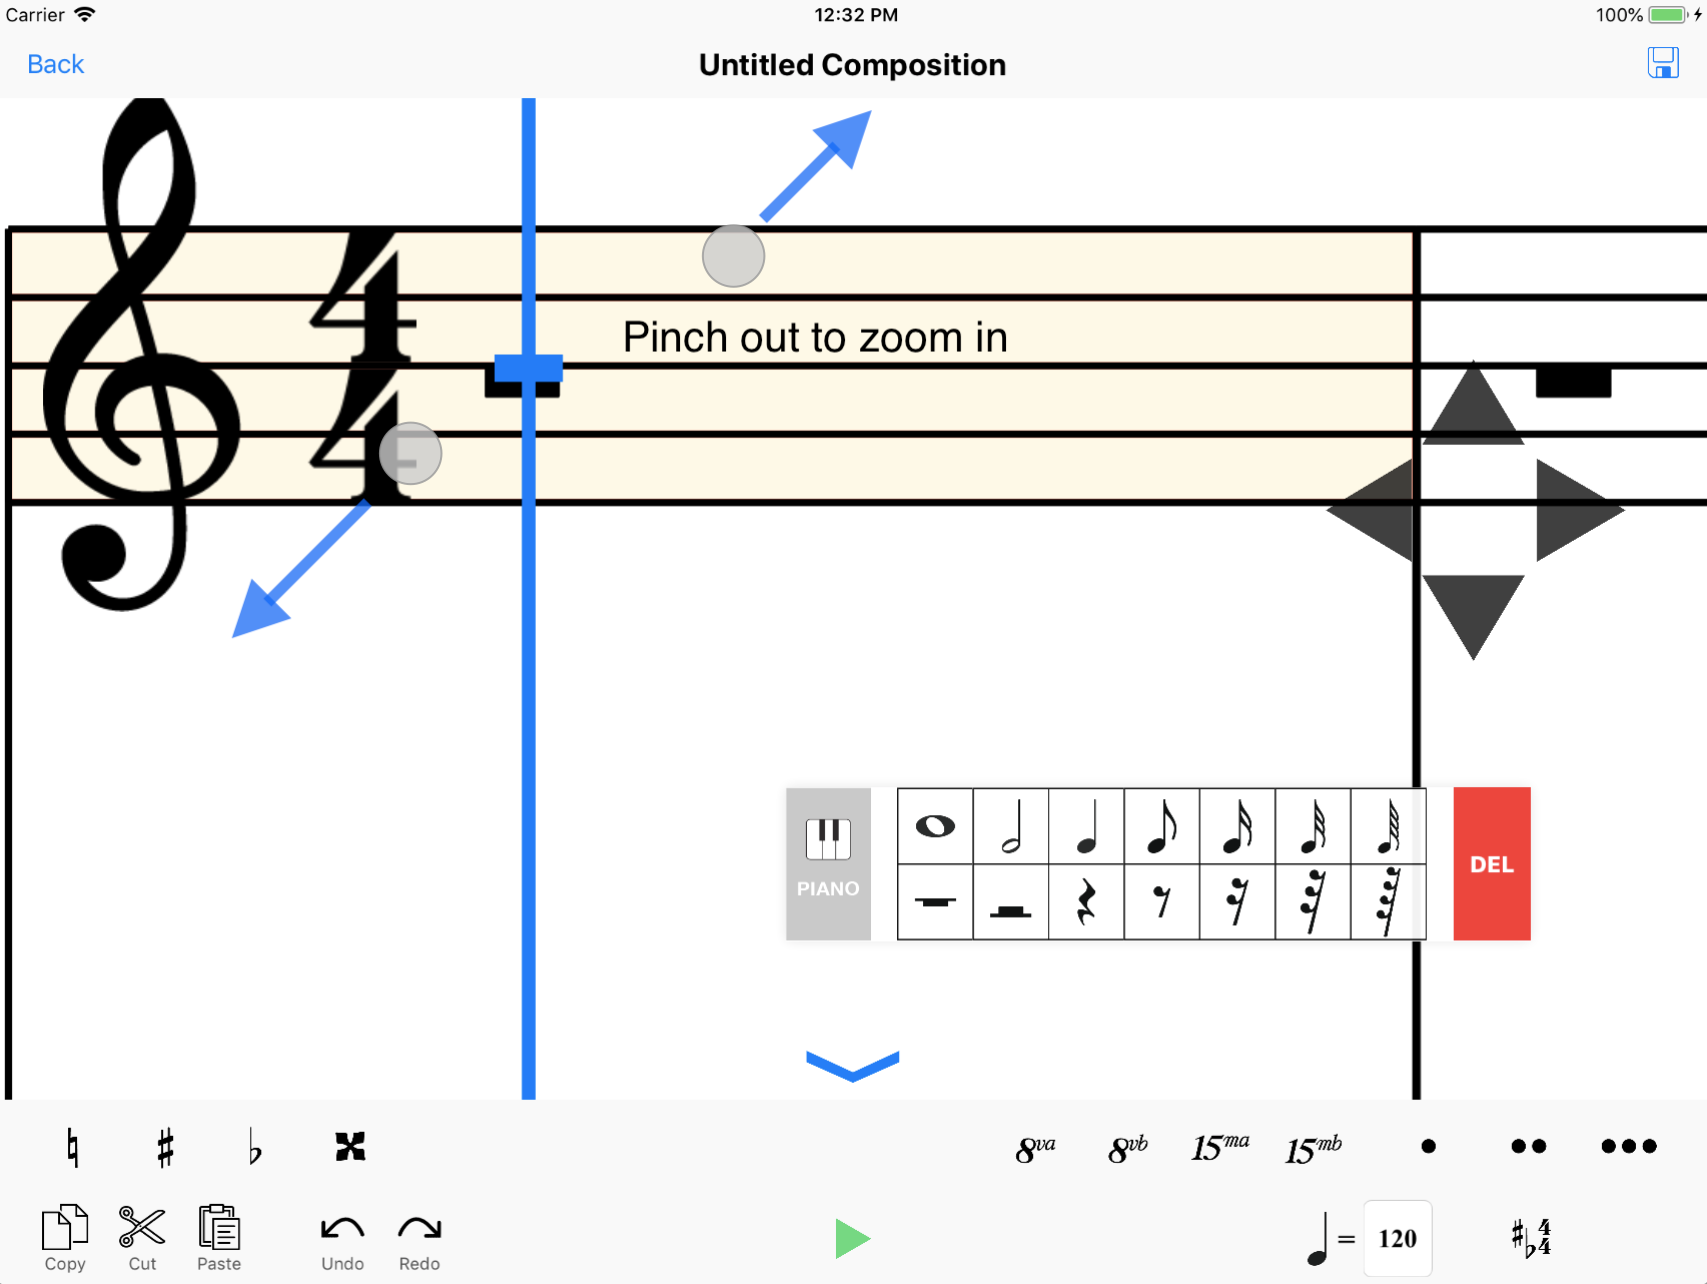
\includegraphics[scale=0.4]{Pinch_Out}
    \caption{Pinch out to zoom in.}
    \label{fig:pinch-out}
\end{figure}

\begin{figure}[H]
	\centering
	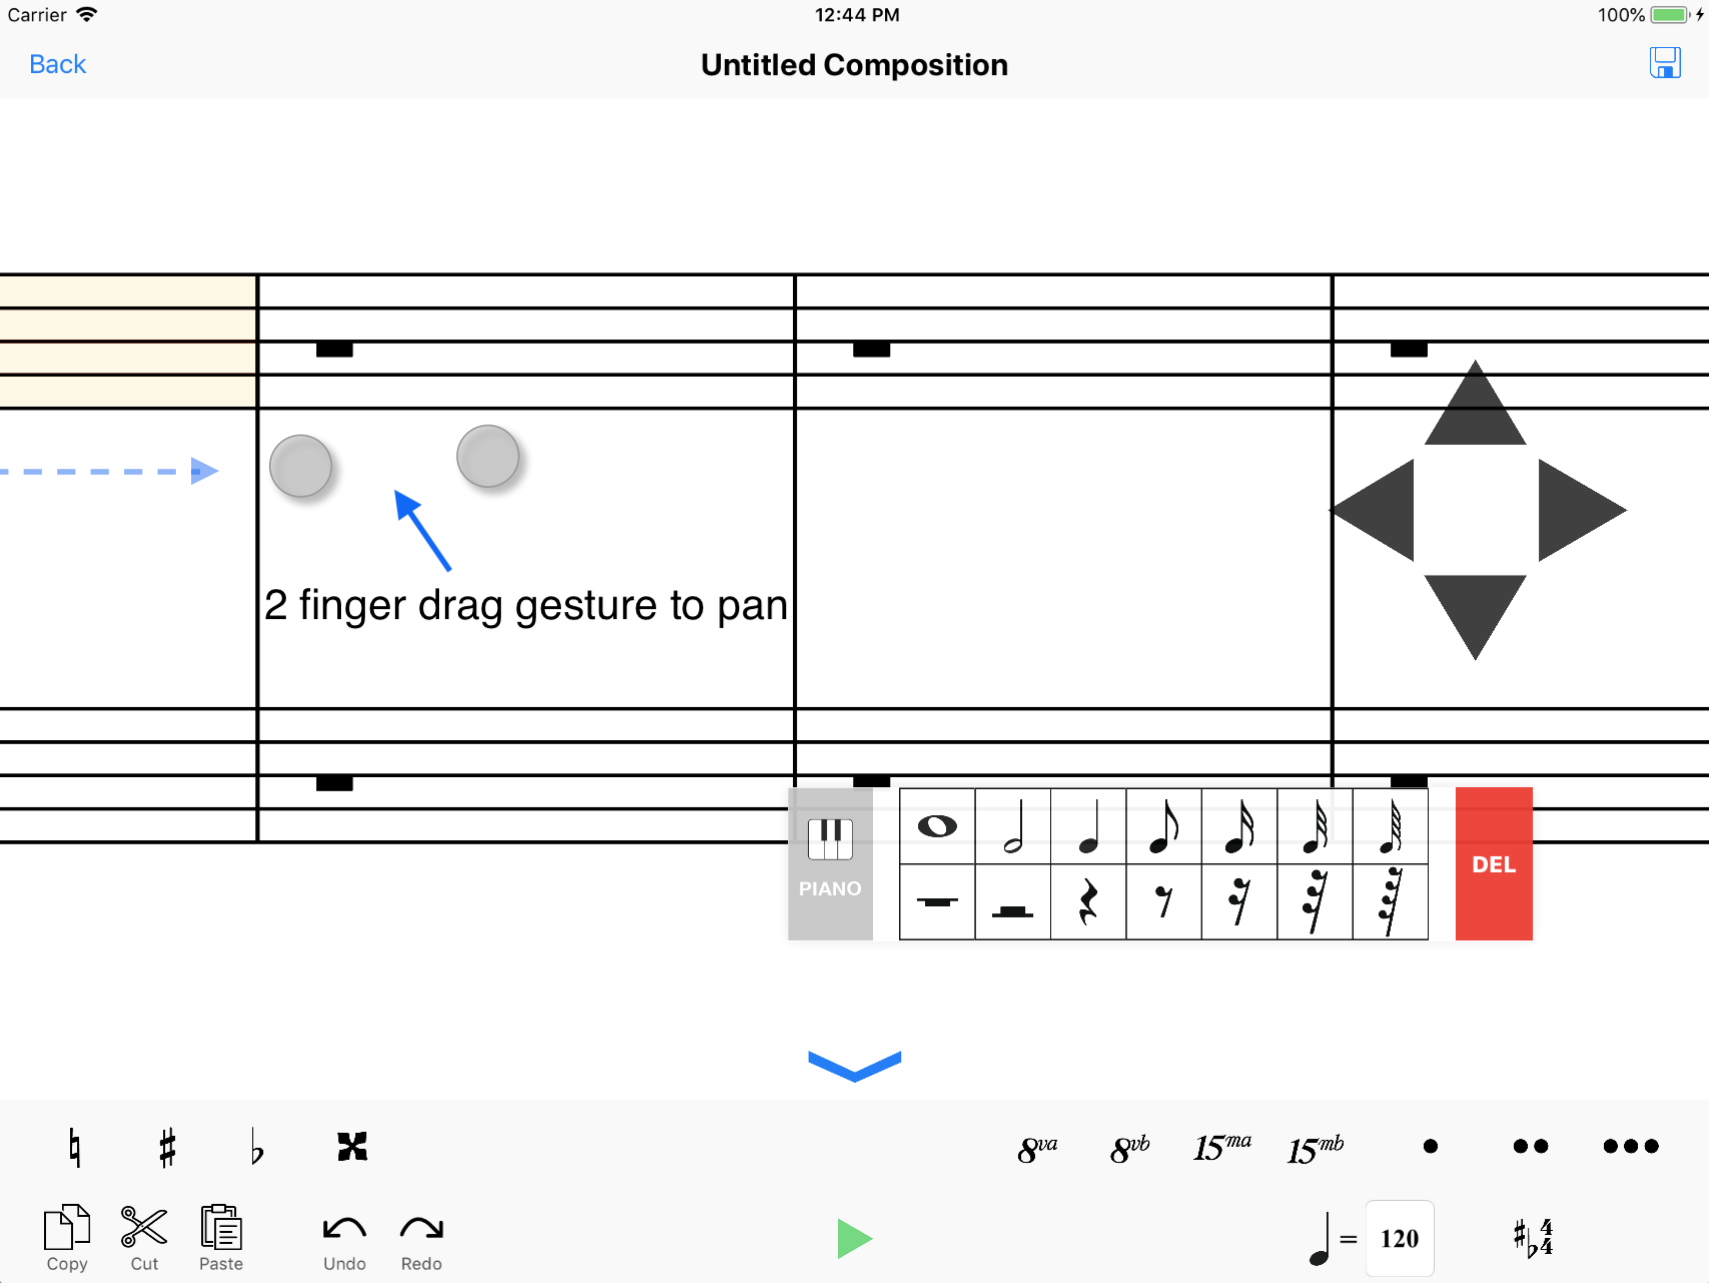
\includegraphics[scale=0.4]{Pan}
    \caption{Two finger drag gesture to pan.}
    \label{fig:pan}
\end{figure}

\subsubsection{Moving the Controls}
The controls in the editor such as the arrow controls and the notation controls are draggable views which allow the user to move them around for flexibility through a 1 finger drag gesture (Figure \ref{fig:move-controls}).

\begin{figure}[H]
	\centering
	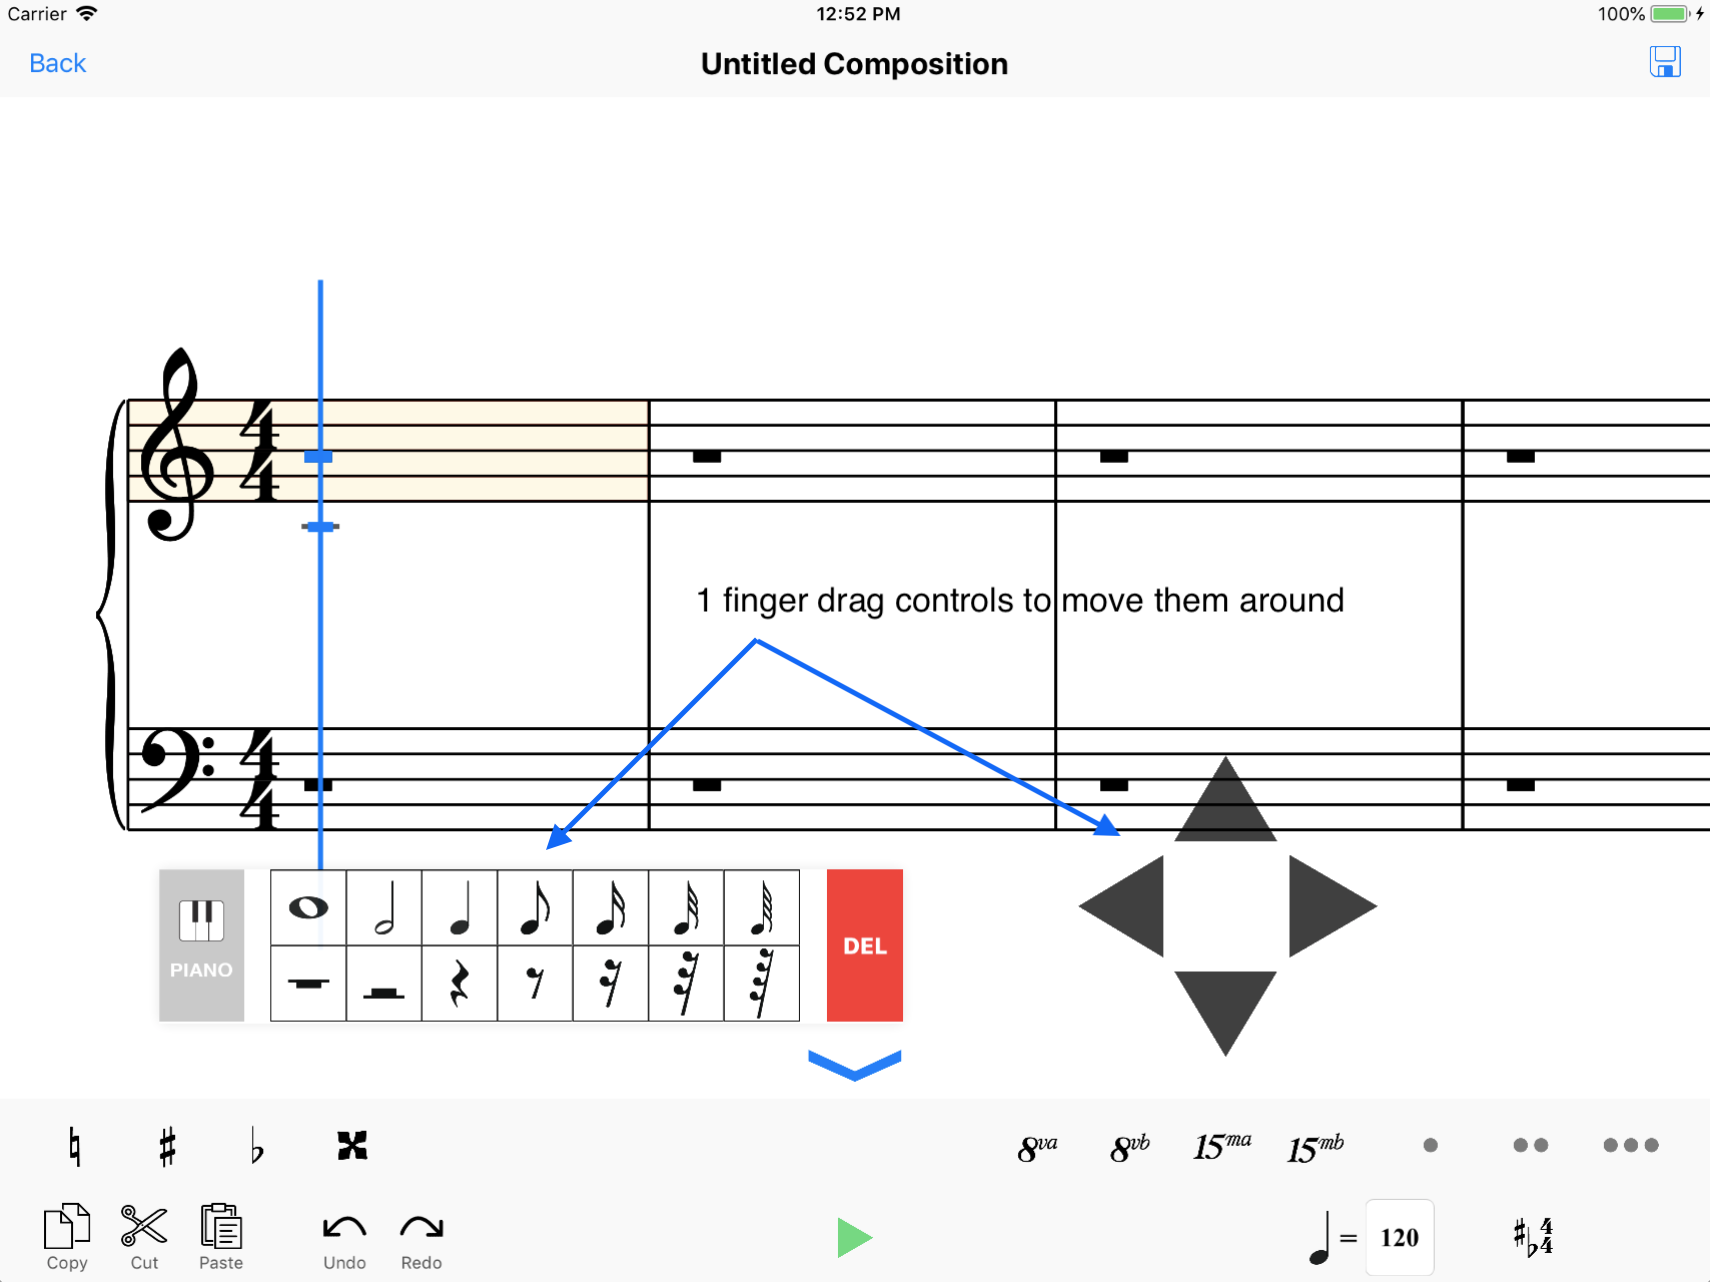
\includegraphics[scale=0.4]{Move_Controls}
    \caption{One finger drag gesture to move controls.}
    \label{fig:move-controls}
\end{figure}

\subsubsection{Renaming a Composition}
Initially, the title of a new composition is set to "Untitled Composition", and the user may edit it by tapping on the title text above in the application toolbar. 

\begin{figure}[H]
	\centering
	
\includegraphics[scale=0.7]{Renaming}
    \caption{Renaming a composition.}
    \label{fig:renaming}
\end{figure}

\subsubsection{Moving the Cursor}
The blue cursor indicates where the next note or rest will be placed, and it also indicates the selected measure and the selected note or rest. There are currently three ways on how the user may move the blue cursor in the editor. The first way is through the use of the arrow controls. Tapping on the up or down arrow keys will change the pitch of the cursor either higher or lower by a half step (Figure \ref{fig:move-arrow-up}). Tapping on the left and right arrow keys, on the other hand, will move the selection of the cursor either to the previous or next note (Figure \ref{fig:move-arrow-right}). The second way of moving the cursor is by dragging it. Upon dragging the cursor, the horizontal line will elongate which indicates that the cursor is already being dragged by the user and also for the user to easily see the current location of the cursor (Figure \ref{fig:cursor-drag}). The third way is by tapping on a location in the editor. Doing so will automatically move the cursor on the tapped location (Figure \ref{fig:cursor-tap}).

\begin{figure}[H]
	\centering
	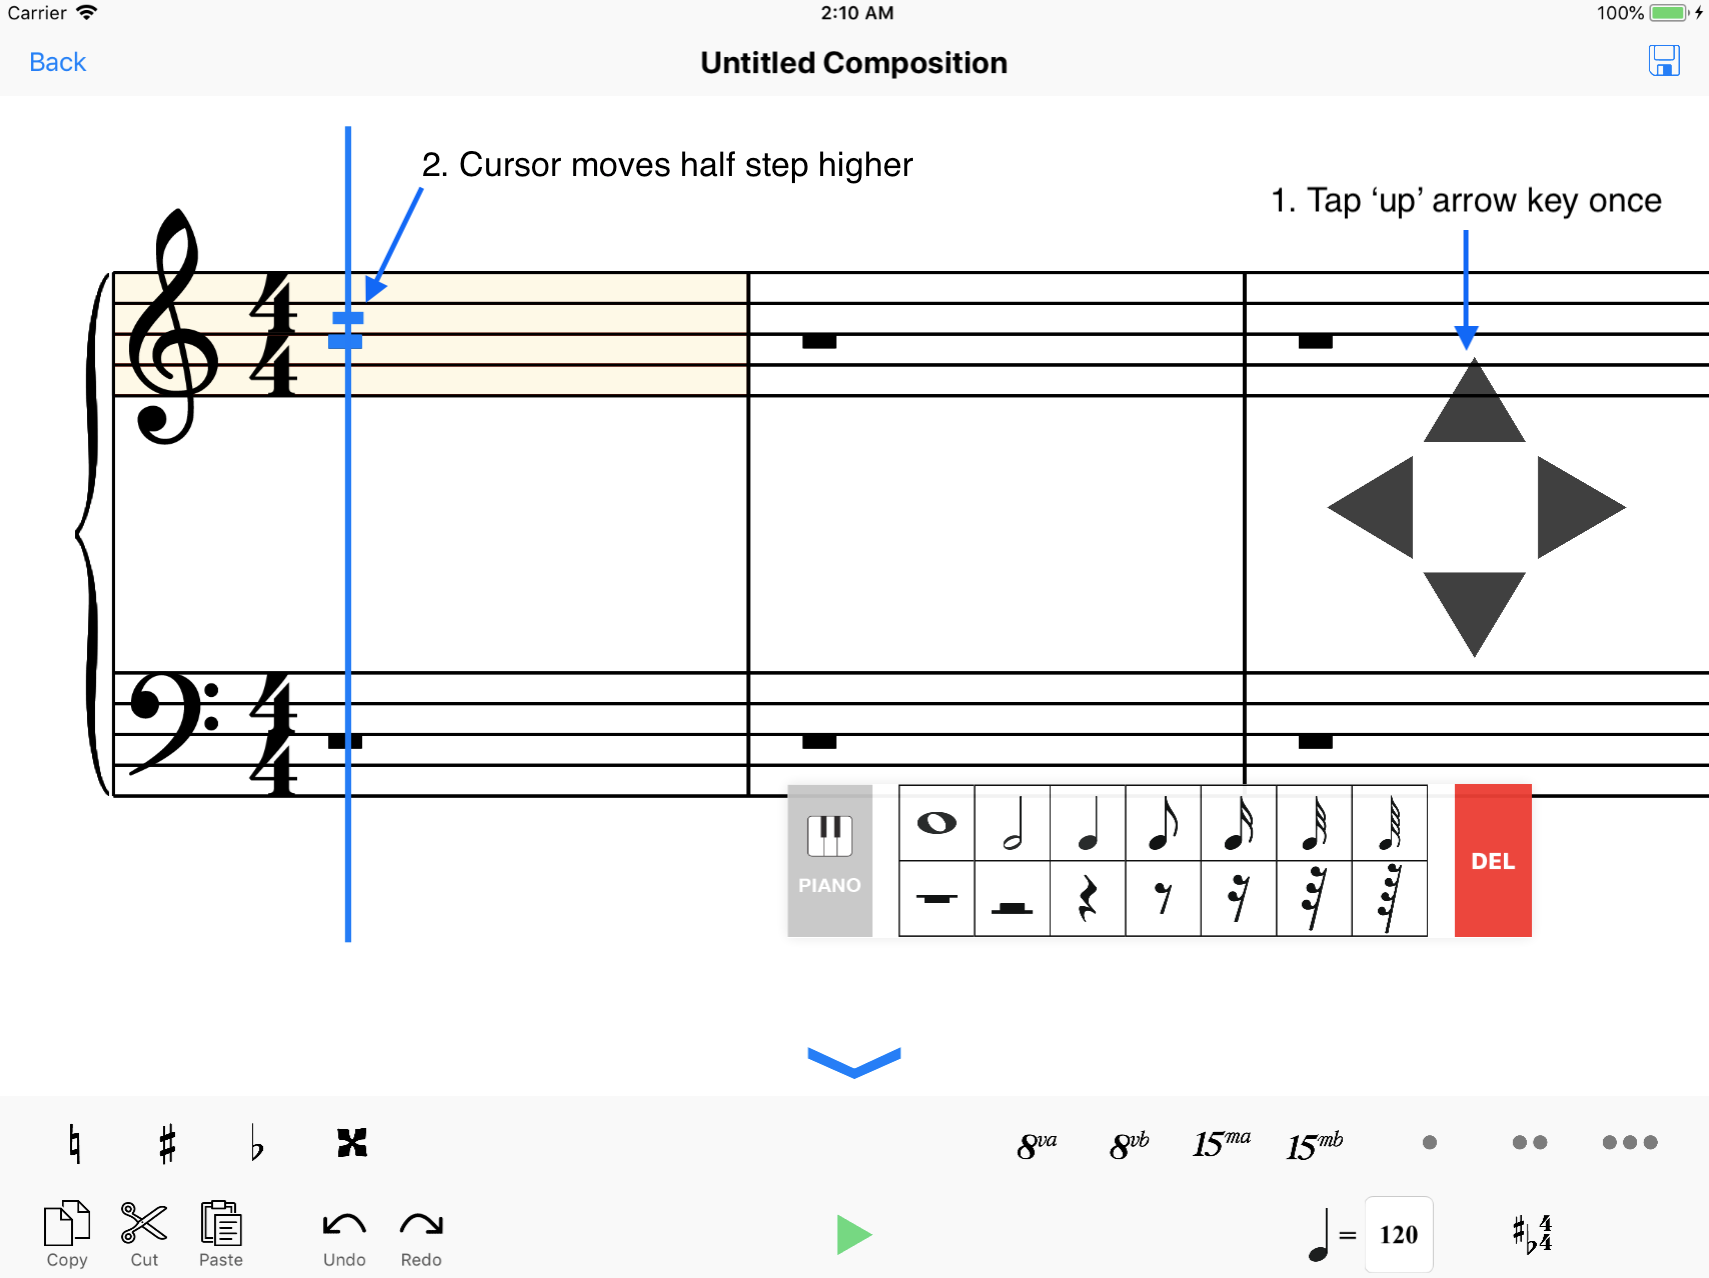
\includegraphics[scale=0.5]{Move_Arrow_Up}
    \caption{Move cursor by a half step higher.}
    \label{fig:move-arrow-up}
\end{figure}

\begin{figure}[H]
	\centering
	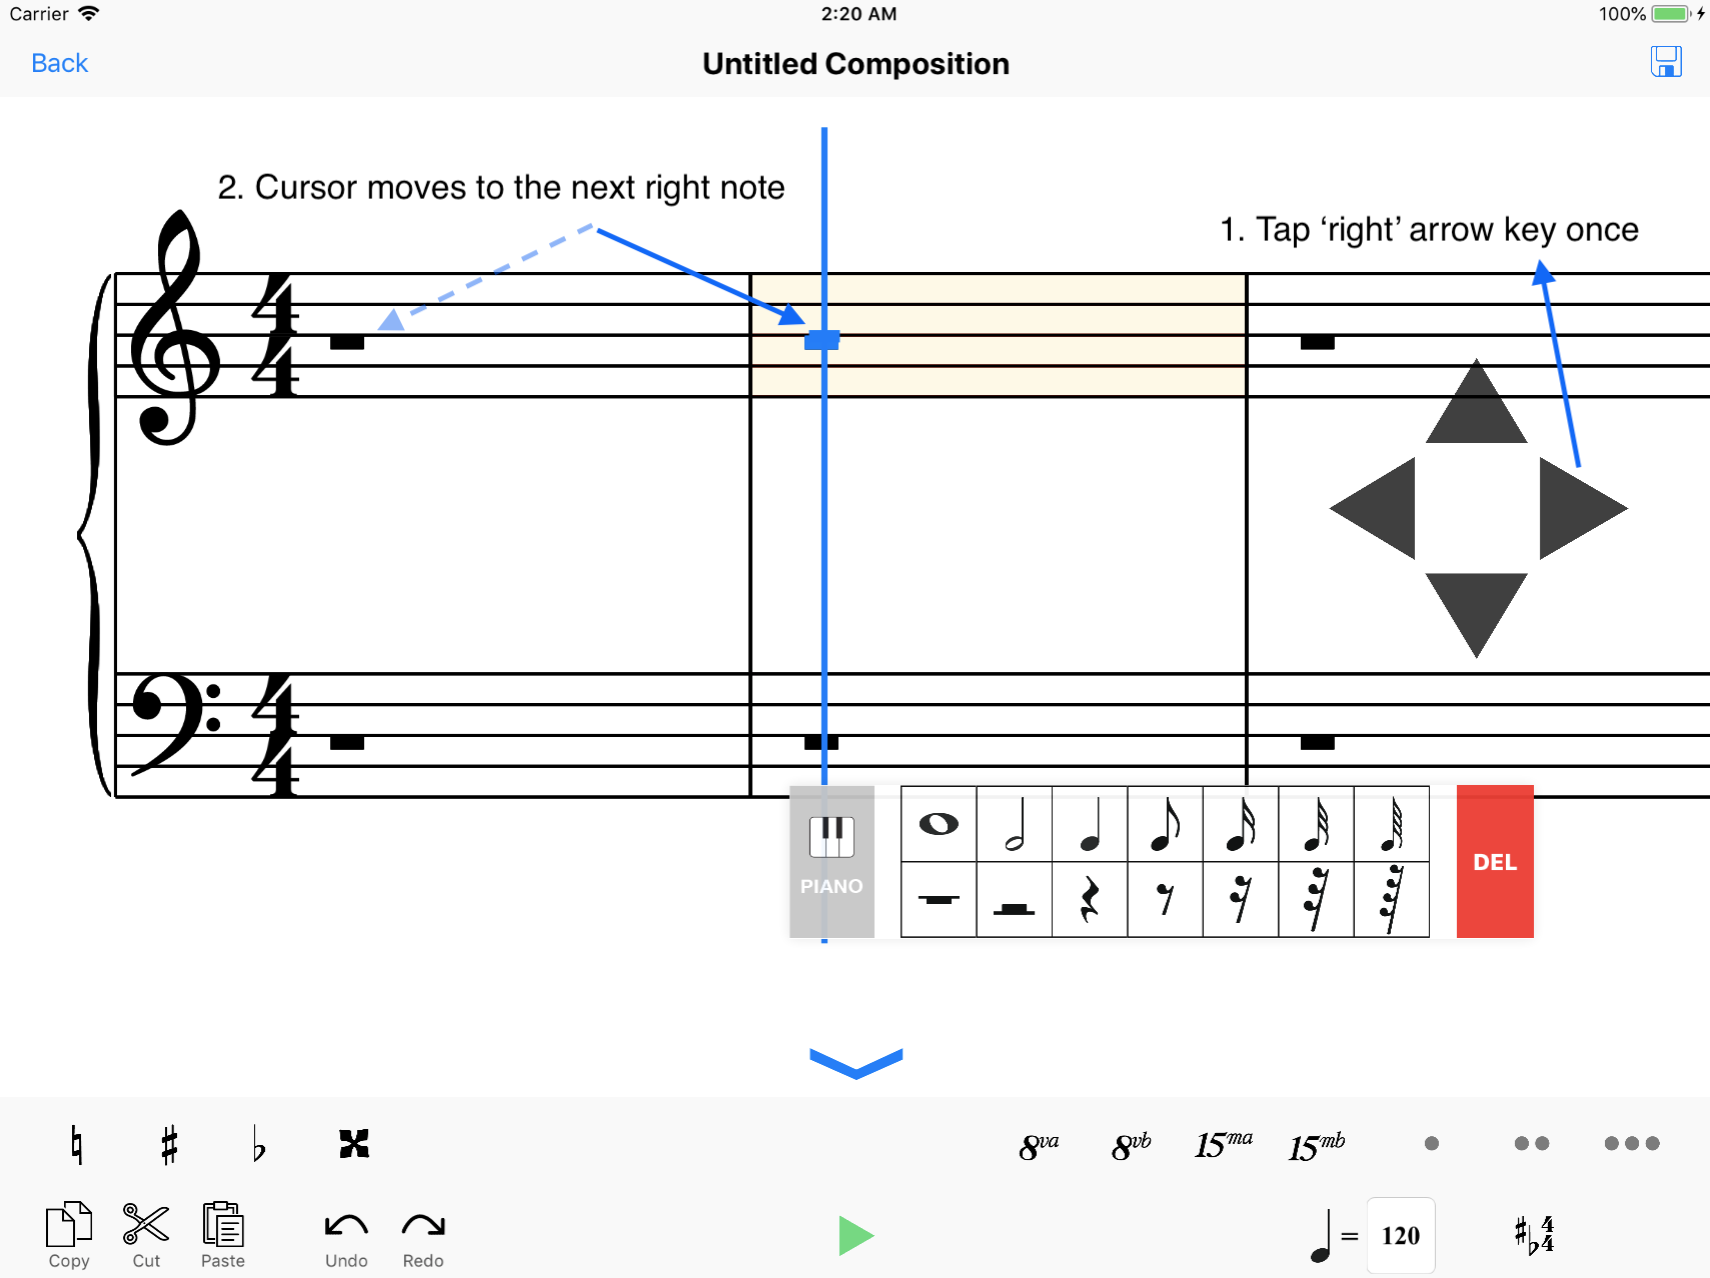
\includegraphics[scale=0.4]{Move_Arrow_Right}
    \caption{Move cursor next note to the right.}
    \label{fig:move-arrow-right}
\end{figure}

\begin{figure}[H]
	\centering
	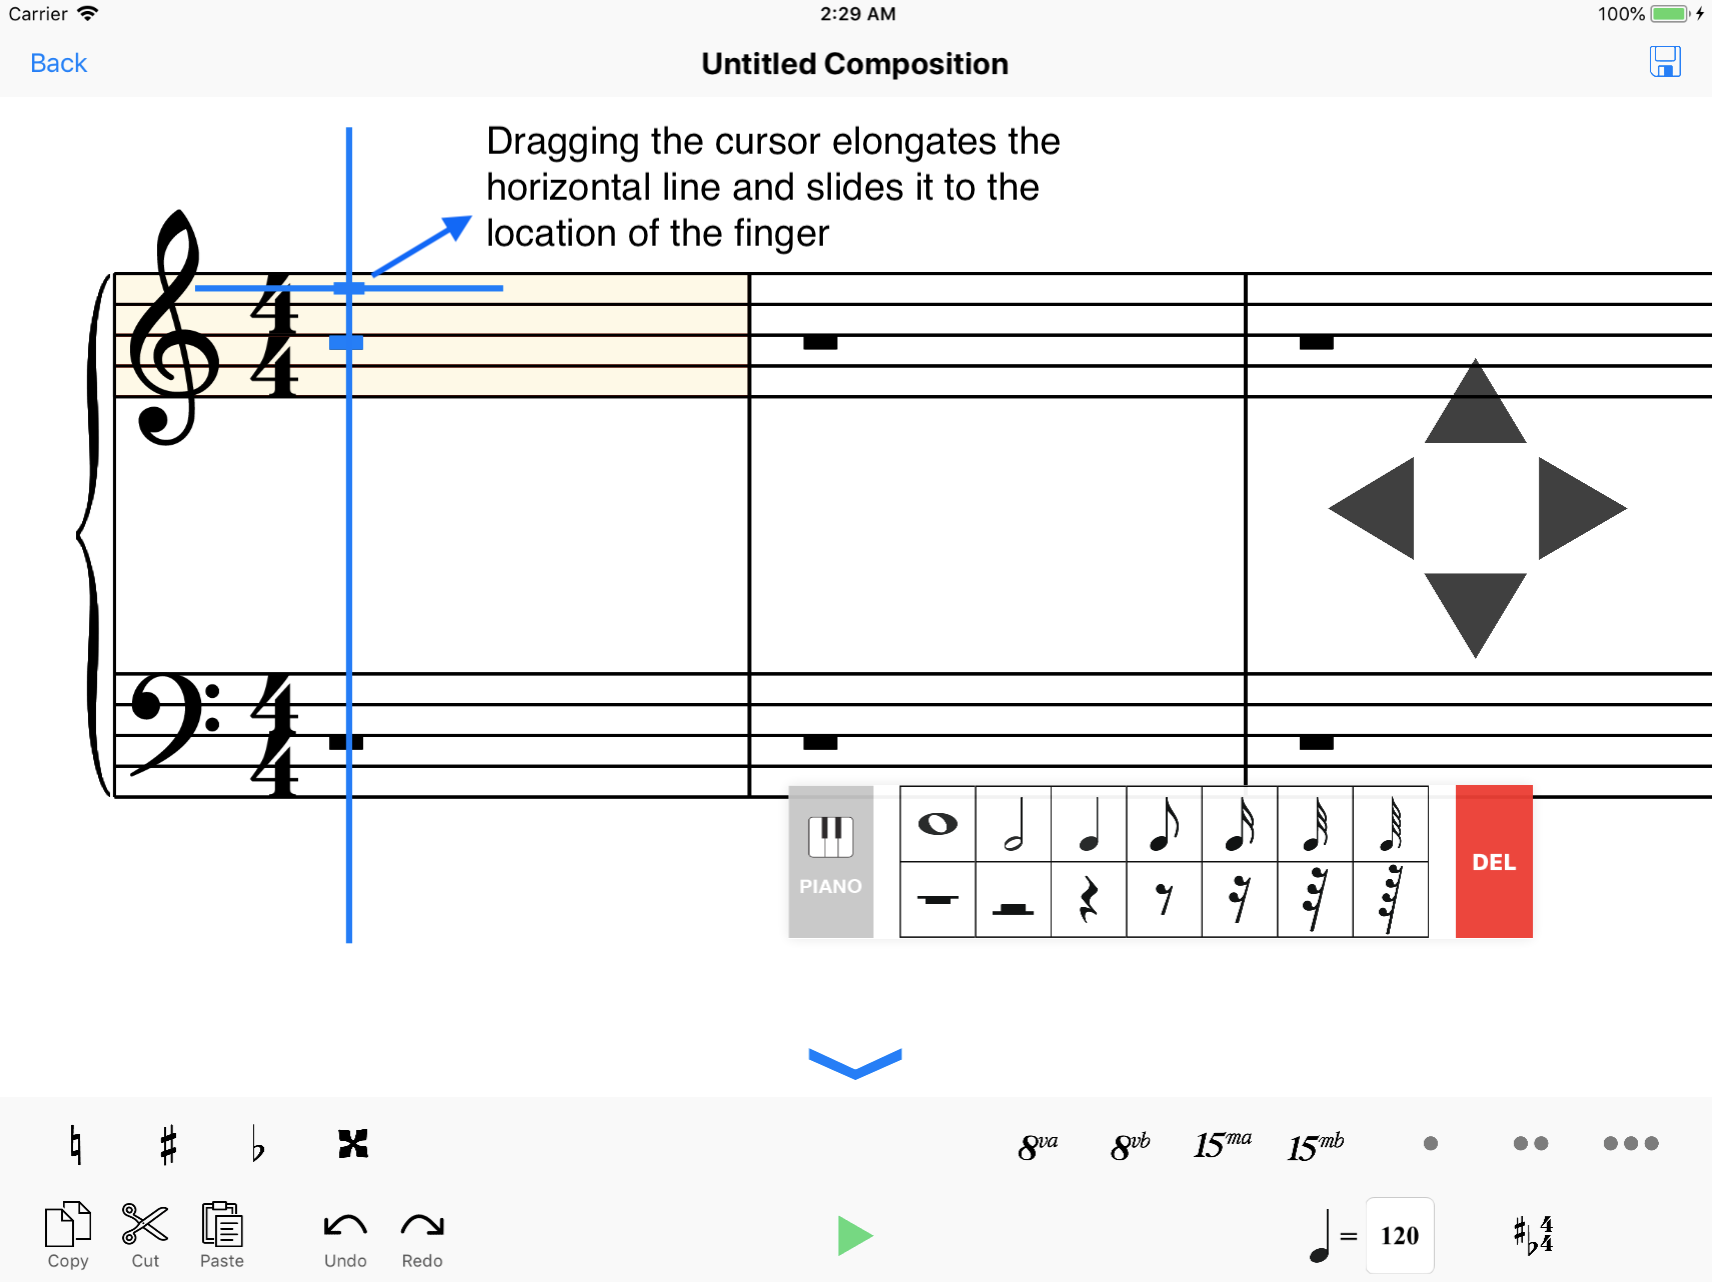
\includegraphics[scale=0.4]{Cursor_Drag}
    \caption{Dragging a cursor.}
    \label{fig:cursor-drag}
\end{figure}

\begin{figure}[H]
	\centering
	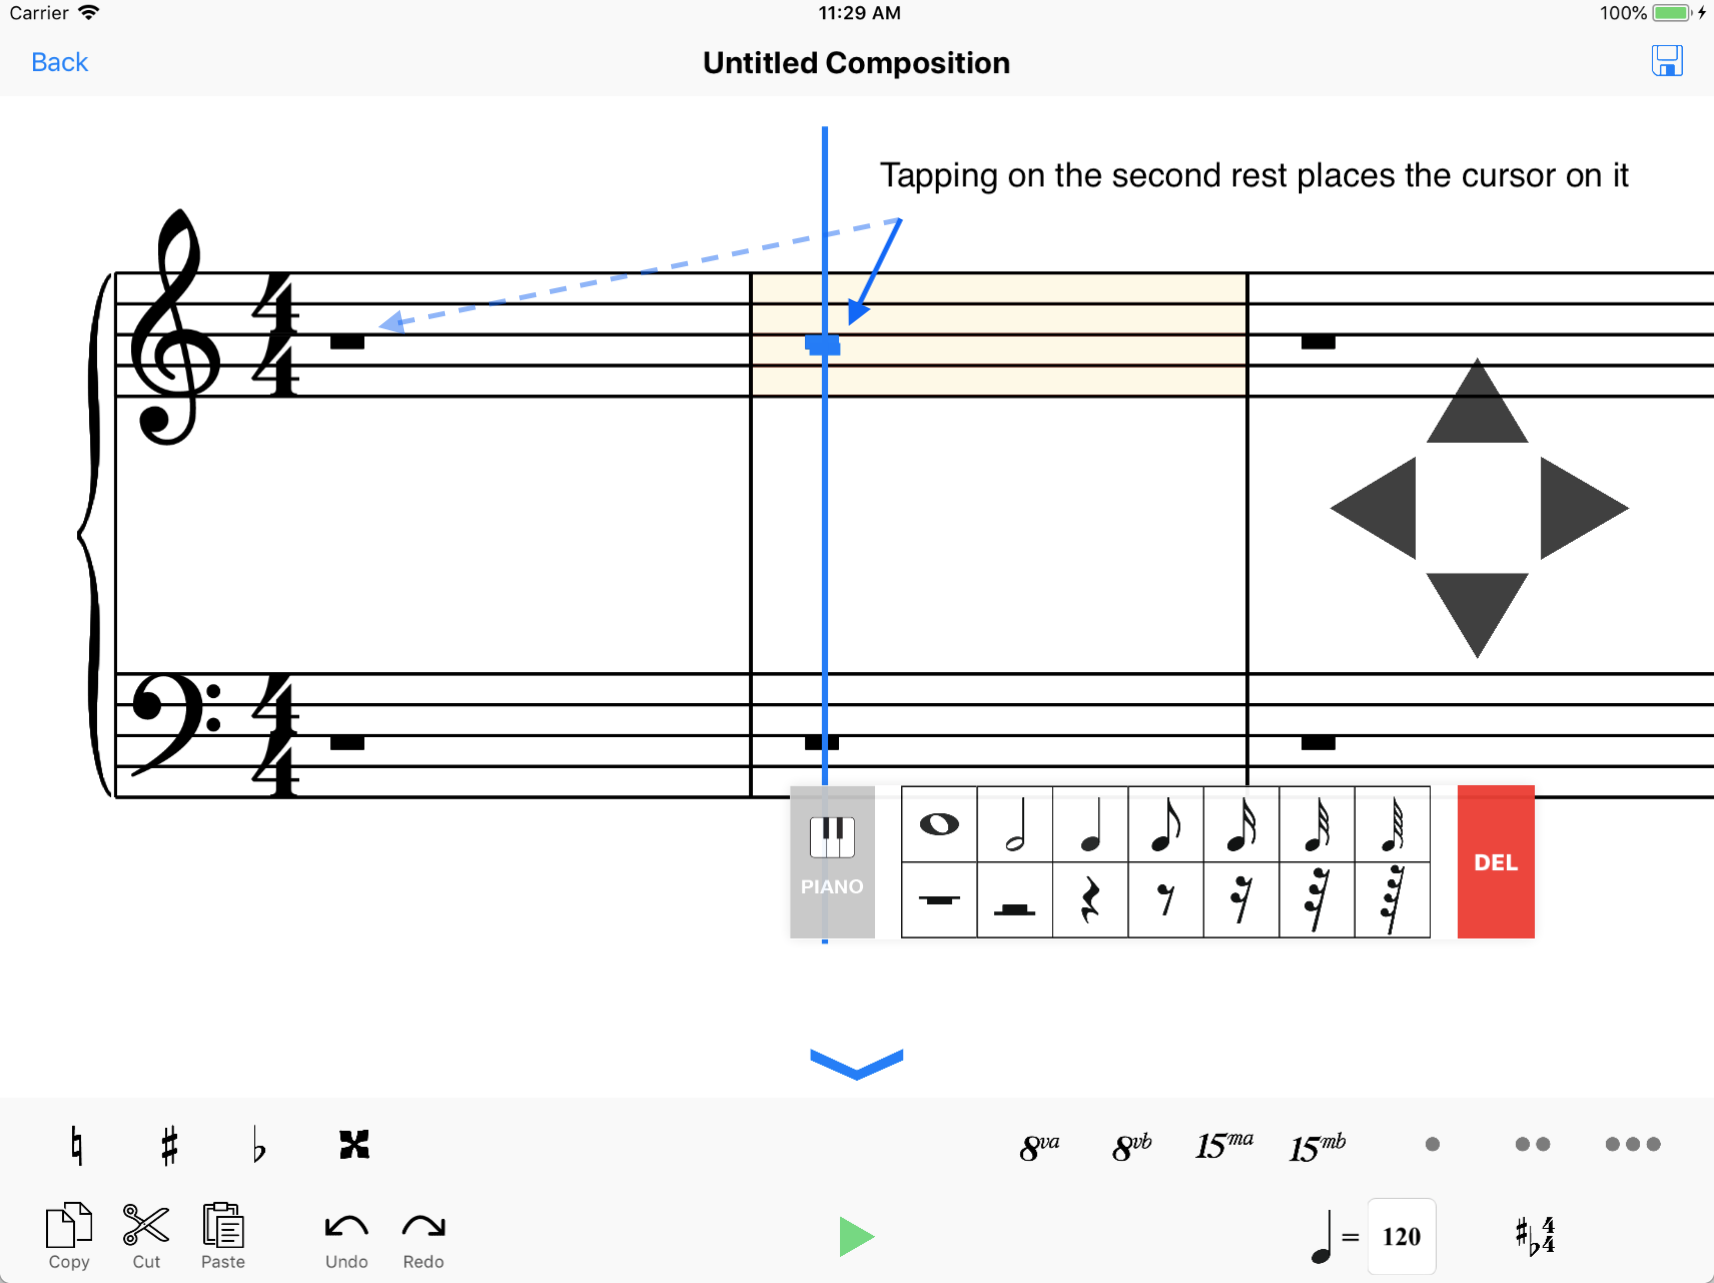
\includegraphics[scale=0.4]{Tap_Cursor}
    \caption{Tap on a location on the editor to move the cursor to it.}
    \label{fig:cursor-tap}
\end{figure}

\subsubsection{Selecting Notes}
A blue highlight on a note or rest indicates that it is currently selected. When a cursor is in the same x-axis with a single note or rest, that note or rest is selected and the user may perform different actions on it such as transpose, edit, or delete (Figure \ref{fig:selected-rest}).

\begin{figure}[H]
	\centering
	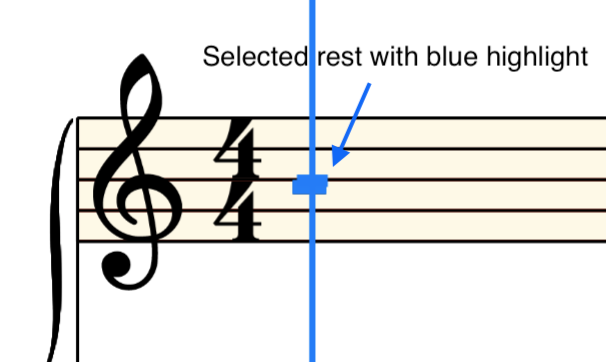
\includegraphics[scale=0.8]{Selected_Rest}
    \caption{Selected rest with blue highlight.}
    \label{fig:selected-rest}
\end{figure}

For selecting multiples notes or rests, the user must do a 1 finger drag gesture in a diagonal direction to bring out the rectangle selector which indicates the area it is currently selecting (Figure \ref{fig:drag-selection}).

\begin{figure}[H]
	\centering
	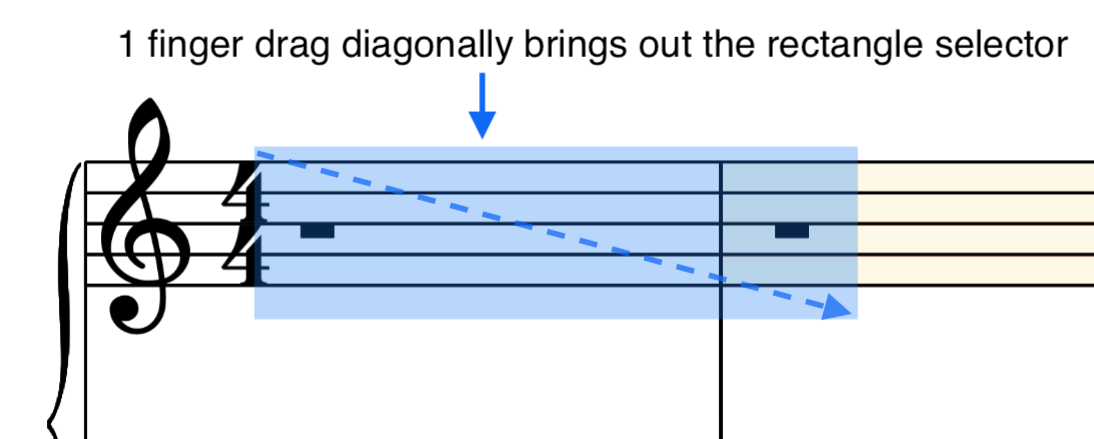
\includegraphics[scale=0.7]{Drag_Selection}
    \caption{1 finger drag diagonally brings out the rectangle selector.}
    \label{fig:drag-selection}
\end{figure}

When the user releases the drag gesture, the rectangle will select the notes it encompassed. Additionally, when more than one rest or note is selected using the drag gesture, it will bring out the transform view which allows the user to transpose, retrograde-inverse, and place a tie or a slur on the selected notes or rests if the rules apply. In the case of Figure \ref{fig:multiple-selected}, the retrograde-inverse and tie or slur buttons are disabled.

\begin{figure}[H]
	\centering
	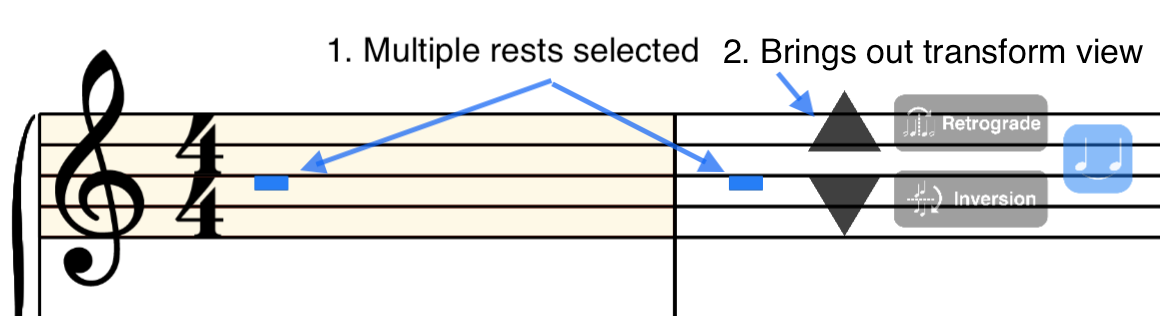
\includegraphics[scale=0.7]{Multiple_Selected}
    \caption{Multiple rests selected with blue highlight and brings out transform view.}
    \label{fig:multiple-selected}
\end{figure}

\subsubsection{Adding a Note or Rest}
Initially, upon creating or opening a composition, the blue cursor automatically selects the first note or rest in the first measure of the composition (Figure \ref{fig:editor}). To add a note or a rest, simply tap on a note type in the notation controls in the editor screen and the note will automatically be added on the location of the blue cursor (Figure \ref{fig:add-note-rest}).

\begin{figure}[H]
	\centering
	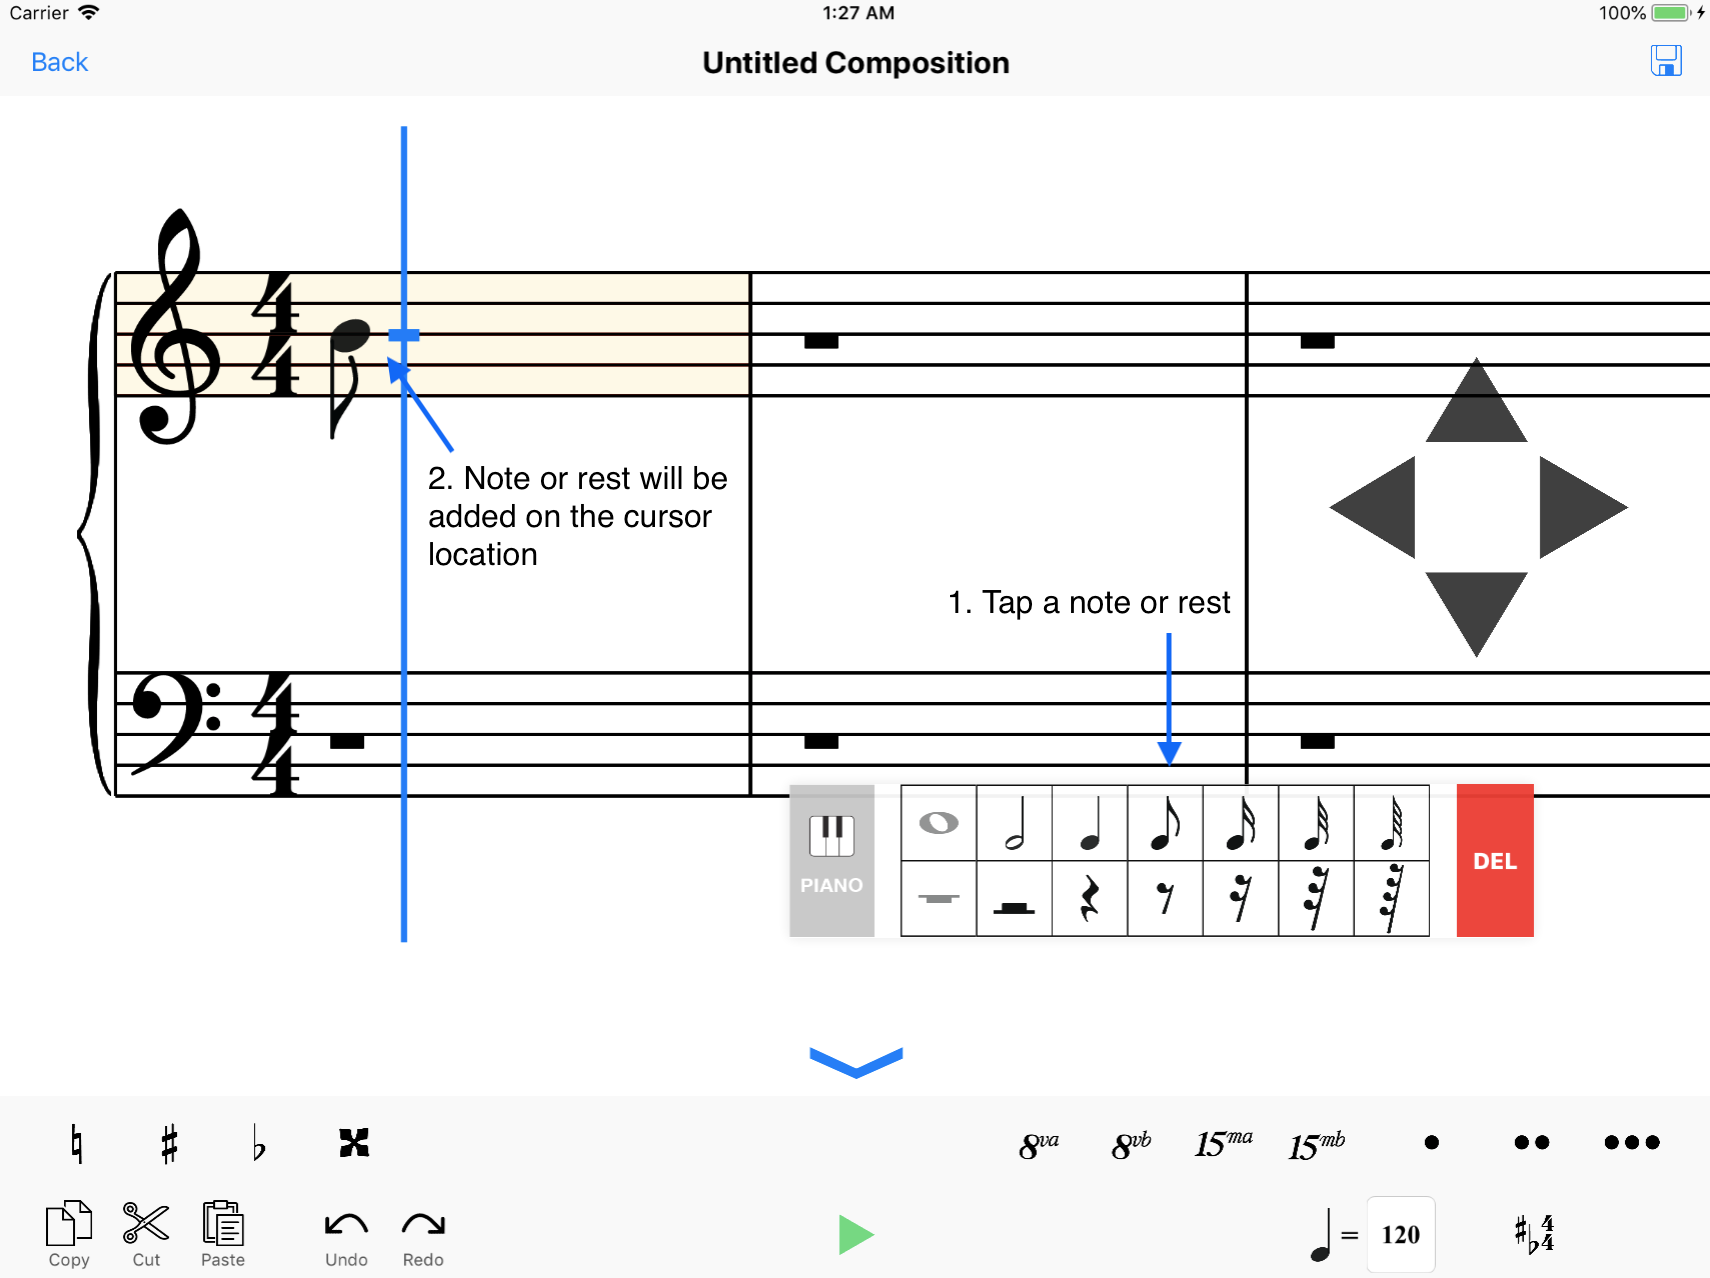
\includegraphics[scale=0.5]{Add_Note_or_Rest}
    \caption{Adding a note or rest.}
    \label{fig:add-note-rest}
\end{figure}

\subsubsection{Adding Polyphony}
To add polyphony, the user must place the cursor above or below an existing note and add a note using the same note type with the existing note.

\begin{figure}[H]
	\centering
	\includegraphics[scale=0.5]{Polyphonic}
    \caption{Adding polyphony.}
    \label{fig:polyphony}
\end{figure}

\subsubsection{Editing Notes}
To edit a note or a group of notes, the user must select the notes that needs editing and tap on the new note type in the notation controls to change the selected notes (Figure \ref{fig:edit-note}).

\begin{figure}[H]
	\centering
	\includegraphics[scale=0.5]{Edit_Note}
    \caption{Editing notes.}
    \label{fig:edit-note}
\end{figure}

\subsubsection{Deleting Notes}
To delete a note or a group of notes, the user must select the notes that needs to be deleted and tap on the delete button in the notation controls to delete the selected notes (Figure \ref{fig:delete-notes}).

\begin{figure}[H]
	\centering
	\includegraphics[scale=0.5]{Delete_Notes}
    \caption{Deleting notes.}
    \label{fig:delete-notes}
\end{figure}

\subsubsection{Transposing a Note or a Group of Notes}
To transpose a note or a group of notes, the user must select the notes that needs to be transposed to show the transpose buttons. Upon selecting the notes, the user may tap on the up or down arrow keys beside the selected notes to transpose them half step higher or lower, respectively (Figure \ref{fig:transposing}).

\begin{figure}[H]
	\centering
	\includegraphics[scale=0.5]{Transposing}
    \caption{Transposing notes.}
    \label{fig:transposing}
\end{figure}

\subsubsection{Retrograde - Inversion}
Retrograde - inversion can be performed only if there are more than one note selected. The transform view beside the selected notes will appear upon selecting notes and the retrograde and inverse buttons will be enabled allowing the user to tap either of them (Figure \ref{fig:r-i}).

\begin{figure}[H]
	\centering
	\includegraphics[scale=0.5]{Retrograde_Inverse}
    \caption{Performing a retrograde or inversion on a group of notes.}
    \label{fig:r-i}
\end{figure}

\subsubsection{Adding Ties or Slurs}
Ties or slurs could be added by selecting more than one note. The transform view beside the selected notes will appear and the tie or slur button will be enabled allowing the user to add a tie or slur on the selected notes. A tie will will be added if the selected notes are all the same pitch, on the other hand, a slur will be added if at least one of the selected notes has a different pitch. Additionally, if a user transposes a note that has a tie or a slur, it automatically changes the type depending whether the connection of all the notes have the same pitch or not (Figure \ref{fig:ties-slur}).

\begin{figure}[H]
	\centering
	\includegraphics[scale=0.5]{Tie_Slur}
    \caption{Adding ties or slurs.}
    \label{fig:ties-slur}
\end{figure}

\subsubsection{Adding and Removing Note Accidentals, Ottava, and Dots}
The accidental buttons are located in the bottom menu of the editor. The behavior of adding and removing accidentals are similar on how the toggling of font types in word processors work. To explain further, an example would be two selected notes that initially do not have any accidentals. After tapping an accidental from the bottom menu with the two notes selected, it would change the type of accidental of all the notes selected. Selected notes with the same accidentals would highlight the accidental button with blue in the bottom menu to show that it could be toggled or tapped again to remove the accidentals in all the notes that are selected (Figure \ref{fig:add-accidental-notes}). In this example, the sharp icon is only added on the first note because the selected notes have the same pitch and the same accidental, but both notes really have a sharp accidental. This is so because of the rules of music notation.

\begin{figure}[H]
	\centering
	\includegraphics[scale=0.5]{Add_Accidental_Notes}
    \caption{Adding accidental on multiple notes.}
    \label{fig:add-accidental-notes}
\end{figure}

Another case would be when a note has a sharp and another note does not have an accidental. When both notes are selected, and the user taps on any accidental, it will change all the selected notes to the tapped accidental (Figure \ref{fig:change-accidental-notes}).

\begin{figure}[H]
	\centering
	\includegraphics[scale=0.5]{Change_Accidental_Notes}
    \caption{Changing accidental on multiple notes with different accidentals.}
    \label{fig:change-accidental-notes}
\end{figure}

Removing accidentals, on the other hand, works by selecting a note with an accidental and tapping the same accidental again. When a single note with accidental is selected, the corresponding accidental button type would highlight blue in the bottom menu and the user may tap it to remove the accidental on the selected note (Figure \ref{fig:remove-note-accidental}).

\begin{figure}[H]
	\centering
	\includegraphics[scale=0.5]{Remove_Note_Accidental}
    \caption{Removing a note accidental.}
    \label{fig:remove-note-accidental}
\end{figure}

There is an alternative way of placing accidentals. This is done by tapping on any accidental button where there is no selected note. When an accidental button is highlighted and no note is selected, all notes that are added will automatically have the accidental selected. To unselect an accidental type, simply place the cursor where there is no note or rest again and tap the highlighted accidental button (Figure \ref{fig:alt-accidental}).

\begin{figure}[H]
	\centering
	\includegraphics[scale=0.5]{Alt_Accidental}
    \caption{Alternative accidental input.}
    \label{fig:alt-accidental}
\end{figure}

The same behavior is implemented for adding and removing ottava and dots.

\subsubsection{Copying, Cutting, and Pasting Notes or Rests}
To copy or cut notes, the user must select the notes first and then tap on the copy or cut button in the bottom menu. After copying or cutting the notes, the user may then tap on the paste button to paste the notes on the location of the cursor (Figure \ref{fig:copy-cut-paste}).

\begin{figure}[H]
	\centering
	\includegraphics[scale=0.5]{Copy__Cut__Paste}
    \caption{Copying, cutting, and pasting notes.}
    \label{fig:copy-cut-paste}
\end{figure}

\subsubsection{Undoing and Redoing Actions}
To undo or redo an action, the user must tap on the undo or redo button in the bottom menu (Figure \ref{fig:undo-redo}).

\begin{figure}[H]
	\centering
	\includegraphics[scale=0.8]{Undo_Redo}
    \caption{Undoing or Redoing actions.}
    \label{fig:undo-redo}
\end{figure}

\subsubsection{Changing the Tempo}
There are two ways of changing the tempo of a composition. The first way is by tapping on the tempo icon in the bottom right part of the menu, and the slider will appear allowing the user to slide it to the left or to the right whilst increasing or decreasing the tempo, respectively (Figure \ref{fig:tempo-slider}). Tapping anywhere outside the tempo slider would hide it.

\begin{figure}[H]
	\centering
	\includegraphics[scale=0.8]{Change_Tempo1}
    \caption{Changing the tempo using a slider.}
    \label{fig:tempo-slider}
\end{figure}

The second way of changing the tempo is by simply tapping on the textbox beside the tempo icon which allows the user to type in the desired tempo (Figure \ref{fig:tempo-type}).

\begin{figure}[H]
	\centering
	\includegraphics[scale=0.8]{Change_Tempo2}
    \caption{Changing the tempo by typing in the textbox.}
    \label{fig:tempo-type}
\end{figure}

\subsubsection{Changing Time Signature and Key Signature}
To change the time signature and key signature of the composition, the user must tap on the time / key signature button (Figure \ref{fig:tim-sig-btn}) on the bottom right part of the menu.

\begin{figure}[H]
	\centering
	\includegraphics[scale=1]{Time_Sig_Btn}
    \caption{Time / Key Signature Button.}
    \label{fig:tim-sig-btn}
\end{figure}

After tapping the time / key signature button, a menu will appear which lets the user set both the time signature and key signature (Figure \ref{fig:tim-sig-menu}). To edit the time signature, the user may tap on one of the preset buttons which will set the values of the number of beats and beat duration automatically. Alternatively, the user may may manually enter the values for the number of beats and beat duration by tapping on their corresponding textboxes. Upon saving the changes of the new time signature, the notes inside the measures that are affected by the change will automatically readjust their location depending on the newly set time signature. In changing the key signature, the user may tap on one of the circular buttons for the key signature. After saving, changes will also affect the notes inside the affected measures.

\begin{figure}[H]
	\centering
	\includegraphics[scale=0.5]{Time_Sig_Menu}
    \caption{Time / Key Signature Menu.}
    \label{fig:tim-sig-menu}
\end{figure}

\subsubsection{Using the Keyboard for Note Input}
The application does not only allow users to add notes through the notation controls, but there is also an alternative way to add notes through the virtual keyboard. To activate the keyboard input, the user must tap on the keyboard button in the left side of the notation controls which brings out the virtual keyboard interface (Figure \ref{fig:keyboard}). After activating the keyboard input, the user may tap on a note type in the notation controls to change the type of note that will be added when pressing a key in the keyboard. Upon pressing a key in the keyboard, the note will be added on the location of the cursor with the corresponding pitch that was pressed on the keyboard and also the selected note type from the notation controls. To deactivate the keyboard input, the user must simply tap on the keyboard button again to hide the keyboard interface and go back to the original method of input.

\begin{figure}[H]
	\centering
	\includegraphics[scale=0.5]{Keyboard}
    \caption{Keyboard input.}
    \label{fig:keyboard}
\end{figure}

\subsubsection{Playing the Composition}
To play the composition, the user must simply tap on the play button on the bottom menu. Playback starts on the currently selected measure and note. The currently selected measure is the measure highlighted with yellow (Figure \ref{fig:play}).

\begin{figure}[H]
	\centering
	\includegraphics[scale=0.5]{Play}
    \caption{Playing the composition.}
    \label{fig:play}
\end{figure}

\subsubsection{Saving the Composition}
To save the composition, the user must simply tap on the save button in the upper right corner of the toolbar (Figure \ref{fig:save}).

\begin{figure}[H]
	\centering
	\includegraphics[scale=2]{Save}
    \caption{Saving the composition.}
    \label{fig:save}
\end{figure}

\subsubsection{Hiding and Showing the Bottom Menu}
To hide the bottom menu, the user must simply tap the arrow facing down on top of the bottom menu (Figure \ref{fig:hide}). To show it back again, the user must tap the arrow key facing up (Figure \ref{fig:show}).

\begin{figure}[H]
	\centering
	\includegraphics[scale=0.5]{Hide}
    \caption{Hiding the bottom menu.}
    \label{fig:hide}
\end{figure}

\begin{figure}[H]
	\centering
	\includegraphics[scale=0.5]{Show}
    \caption{Showing the bottom menu.}
    \label{fig:show}
\end{figure}

\section{Experiment Design}

This chapter will describe the user stories and use cases that will be highlighted in the testing of the application. The intended users for the application will be expert composers who have at least 7 years of experience with composing music and amateur composers who have less than 7 years of experience composing music. These users should also have a basic knowledge of musical terms and are able to read and write musical notation. The details on the testing to be conducted on these users will also be discussed in this chapter.

\subsection{User Stories}
The user stories of the system will be focused on the main functions of the application and will highlight each specific need that the user has for the system. These user stories came from the users, representing the tasks that they need to perform on musical composition applications. These are created with the context that the system will run on a mobile platform with the mode of interaction mainly being touch gestures. 

\begin{enumerate}
\item As a user, I want to be able to create a blank composition, so that I can start my work
\item As a user, I want to be able to name my composition, so that I can differentiate it from my other compositions
\item As a user, I want to be able to save my composition, so that I can come back to it later
\item As a user, I want to be able to view all my saved compositions in a list, so that I can keep track of everything
\item As a user, I want to be able to open a saved composition so that I can perform more actions on it
\item As a user, I want to be able export my composition in a format that I can open in the composition application I use on my laptop
\item As a user, I want to be able to delete a composition, so I can discard compositions I do not work on anymore
\item As a user, I want to be able to add a chord progression in my composition, so that I do not need to individually add notes that belong to a progression
\item As a user, I want to be able to place a note in my composition, so that I can create my composition
\item As a user, I want to be able to select a single note, so that I can perform actions on it
\item As a user, I want to be able to change the pitch class of a note in my composition, so that I can make adjustments to my composition
\item As a user, I want to be able to change the type of a note in my composition, so that I can make the sound longer or shorter
\item As a user, I want to be able to erase a note in my composition, so that I can make space for other notes in my composition
\item As a user, I want to be able to highlight a group of notes in my composition, so that I can perform actions on the group
\item As a user, I want to be able to erase a highlighted group of notes in my composition, so that I can make space faster for other notes I'd like to place in my composition
\item As a user, I want to be able to place a rest in my composition, so I can have pauses in my composition
\item As a user, I want to be able to select a rest, so that I can perform actions on that rest
\item As a user, I want to be able to change the type of rest, so that I can change the length of pauses
\item As a user, I want to be able to highlight a group of rests, so that I can perform actions on the group of rests
\item As a user, I want to be able to erase a rest in my composition, so that I can make space for other rests or notes
\item As a user, I want to be able to change a rest in my composition, so that I can make adjustments to my composition
%\item As a user, I want to be able to move the position of a note in my composition, so that I can move that note to a better position
%\item As a user, I want to be able to move the position of a highlighted group of notes in my composition, so that I can reposition multiple notes at a time to a better position
\item As a user, I want to be able to hear the sound of the note I just added, so that I know I've added the correct sounding note
\item As a user, I want to be able to listen to a highlighted section of my composition, so that I can hear just a segment of my piece
\item As a user, I want to be able to listen to my whole composition, so that I can hear it as a whole
\item As a user, I want to be able to perform a swipe gesture that will generate a succession of notes based on the orientation of my gesture and my current composition because I'm interested in knowing what series of notes match my current composition
\item As a user, I want to be able to manipulate the generated series of notes, because the generated series of notes just needs a little bit more adjustments before I accept it into my composition
\item As a user, I want to be able to discard the series of notes generated by the application after a swipe gesture, so I do not have to delete them one by one
\item As a user, I want to be able to confirm the addition of the series of notes given by the application after a swipe gesture, so I can create my composition quickly
\item As a user I want to be able to undo an action or a series of actions, so that I can undo an unintended action or series of unintended actions quicker
\item As a user I want to be able to redo an action or a series of actions, so that I can redo an intended action or a series of intended actions quicker
\item As a user, I want to be able to reposition the menu because I want to place it where it is not an obstacle for me while composing
\item As a user, I want to be able to set the time signature of my composition
\item As a user, I want to be able to see the details of a single note, so that I can know the specifications of the note
\item As a user, I want to be able to see the details of a selected group of notes, so that I can know the specification of the selected group of notes
\item As a user, I want to be able to see the details of the generated series of notes like the pitch and type so that I can know what notes the system has generated after a gesture
\item As a user, I want to be able to set the clef of my composition
\item As a user, I want to be able to set the key signature of my composition
\item As a user, I want to be able to set the time signature of my composition
\item As a user, I want to be able to copy a highlighted group of notes and/or rests, so that I can copy a recurring segment in my composition
\item As a user, I want to be able to cut a highlighted group of notes and/or rests, so that I can copy a segment of my composition while at the same time making space for more notes
\item As a user, I want to be able to paste the copied or cut group of notes and/or rests onto my composition, so that I do not need to add a recurring segment in my composition manually all the time
%\item As a user, I want to be able to move the position of a rest, so that I can move that rest to a better position
%\item As a user, I want to be able to move the position of a selected group of rests, so that I can move multiple rests at a time to a better position
\item As a user, I want to be able to add accidentals to my notes, so that I can control the pitch of my notes
\item As a user, I want to be able to transpose a highlighted group of notes, so that I do not need to individually change the pitch of each note
\item As a user, I want to be able to perform retrograde inversion on a single note, so that I do not have to move it manually to invert it
\item As a user, I want to be able to perform retrograde inversion on a group of notes, so that I do not need to invert each note individually

\end{enumerate}

\subsection{User Test Plan}

The objective of the tests will be to determine if the interaction and design of the system augments the user experience of the composer while interacting with Flow. The functionality will also be closely monitored to see if there are glitches or bugs that require additional fixes in the development side. These bugs or glitches will warrant an intervention from the researchers during the testing.

The tests will be conducted in an environment where audio and visual disturbances are at a minimum. This is to ensure that the researchers are able to analyze clear audio and video data from the recording devices used during the testing. This is also to ensure that the tester is not disutbred during the testing. The setups used accross all the user tests are 4 kinds of Flow system prototpyes, 1 created using a prototyping tool called InVision, and 3 coded in Swift; 2 kinds of commercially available notation applications in the App Storem, Notion and Komp; and the traditional form of composition which is using music sheets and writing materials. Notation softwares and the Flow prototypes will be launched on a mobile platform, namely an IPad tablet.

Before starting the test, testers will be given a consent form. If they agree with the terms and continue with the testing, the tasks indicated in Section \ref{sec:tasks} will be done for each test setup (indicated in Section \ref{sec:test-setups}) that is appropriate. Before the start of the test where the tester start to accomplish tasks or use cases for the test setup, they will be given a brief description of the objectives of the study along with overview of the tasks or use cases. 

The researchers will be collecting quantitative and qualitative data. There will be tasks that the testers will be asked to accomplish, during iteration 1 and 2, after those tasks, data will be collected through an online form open after testing. During iteration 3 and 4, data will be collected during each use case through an online form. There will be video recording of the testers face and hand movements to be analyzed by the researchers during the testing. After the testing, for iteration 1 and 2, testers are then asked to answer a questionnaire to evaluate the quality of the application, and for iteration 3 and 4, testers are given a brief interview about their thoughts on each of the setups and the application.

During the first two (2) iterations, five (5) subjects of both genders aged 18-40 were recruited through snowball sampling method to take part in the data collection and testing. These subjects were categorized into two (2) user groups based on musical composition experience: amateur, and experienced. For the third iteration, fifteen (15) subjects of the same demographics took part in the testing. In the last iteration, ten (10) subjects took part. 

\subsection{Test Setups}
\label{sec:test-setups}

The setups between the preliminary testing and the subsequent testing were different. This was made so because the main goal of the preliminary testing was to gather feedback on the interaction design and help improve the system while it was still being developed. Other applications did not matter as much and were only used to gain insight on their interactions and how they could be used to improve the system. Although the goal of the subsequent tests were still to gather feedback and improve the system, they were also made to compare the system against similar musical composition applications. 

\subsubsection{Preliminary Testing Setups}

The test setups are meant to observe how existing methods of composition work and how their interactions could be used in Flow. The tasks enumerated in Section \ref{sec:preliminary-tasks} will be used in each test setup whenever possible since some tasks can only be accomplished within a specific setup. 

There will be 3 different test setups to be used during user testing namely:

\begin{enumerate}
\item Tester composing using music sheets
\item Tester composing using Komp
\item Tester composing using Flow
\end{enumerate}

The first setup simulates the traditional way of musical composition. This is through music sheets and a writing instrument. Traditional music sheets will be provided by the researchers as well as a choice of using a pen or pencil for writing musical elements. The composers are free to use as much music sheets as they want for drafting and experimenting with their composition as long as the time and resources provided by the researchers allow them.

The second setup will be through an existing mobile application for iOS platforms, komp. Since the method of input in komp is similar to writing in music sheets, this setup will mainly be done to see how the interaction for traditional musical composition will work when applied to mobile devices. The researchers expect this setup to have similar results with the first setup and any data collected in this setup will be used to evaluate Flow.

The third setup will be focused on the composer using the developed system, Flow. During the early periods of testing, a mid-fidelity InVision prototype will be used as a substitute. Using this prototype, the only task that the composer will be able to do is to explore the application. The main goal of this is to develop and improve the interaction design of the application. One a high-fidelity prototype has been developed, all tasks will be performed in the testing.

\subsubsection{Subsequent Testing Setups}

In the subsequent tests, Flow was compared against other musical notation applications. For each setup, the users had to go through the use cases listed in \ref{sec:use-cases} and perform the tasks outlined in \ref{sec:subsequent-tasks}. Note that these setups were given in random order and that the application developed by the researchers was not disclosed to prevent bias.

\begin{enumerate}
\item Tester composing using Notion
\item Tester composing using komp
\item Tester composing using Flow
\end{enumerate}

The first setup makes use of what is said to be the most popular musical notation application for mobile. For the second setup, komp is retained from the preliminary testing so that users can experience a traditional method of notation while on the iPad. The last setup makes use of the system developed by the researchers.

\subsubsection{Use Cases}
\label{sec:use-cases}

For the subsequent test setups, the testers had to go perform use cases. These use cases were an attempt to simulate different musical composition scenarios. 

\begin{enumerate}
    \item Compose a familiar song (Twinkle Twinkle Little Star/Happy Birthday)
    \item Compose from scratch
    \item Modify a composition (Ode to Joy/Amazing Grace)
\end{enumerate}

\subsection{Tasks}
\label{sec:tasks}

Similar to the test setups, the tasks differed greatly between the preliminary testing and subsequent testing. Tasks were generalized in the subsequent testing to make it easier for the testers to compare the different applications.

\subsubsection{Preliminary Testing Tasks}
\label{sec:preliminary-tasks}

Some tasks may be omitted in different test setups when a crucial function to carry out the task is unavailable. During the final task, testers are encouraged to speak aloud their concerns and opinions regarding the application.

For the first iteration, there will be 4 tasks for each of the setups with 1 special task for the setup using Flow:
\begin{enumerate}
\item Add a Note
\item Add a Series of Notes
\item Change a Note
\item Special Task - Delete a Series of Notes
\item Compose for 3 Minutes
\end{enumerate}

For the second iteration, there will be 7 tasks for each of the setups setups and 3 additional special tasks for the setup using Flow:
\begin{enumerate}
\item Add notes to fill 2 measures
\item Change Time Signature to 3/4
\item Special Task - Empty one measure
\item Special Task - Empty composition
\item Add enough notes to fill 2 measures in 2 staffs
\item Add an accidental to 2 notes
\item Remove placed accidentals 
\item Change Key Signature
\item Special Task - Replace a group of notes with a single note
\item Create or recreate a composition (Exactly 4 measures)
\subitem Twinkle Twinkle Little Star
\subitem Canon in D
\subitem Ode to Joy 
\end{enumerate}

\subsubsection{Subsequent Testing Tasks}
\label{sec:subsequent-tasks}

Since one of the goals of the subsequent tests was to compare how the interaction was against similar applications, the tasks were greatly simplified and generalized. Testers were also allowed to perform the tasks in any order they wanted and as much repititions it took for them to get acquainted with the specific task or action. These tasks were repeated for each of the use cases mentioned in \ref{sec:use-cases}.

\begin{enumerate}
  \item Select/highlight notes/chords
  \item Add notes/chords
  \item Edit notes/chords
  \item Delete notes/chords
  \item Cut, copy, or paste notes/chords
  \item Undo/redo an action
  \item Play the composition
\end{enumerate}
\end{comment}


%!TEX root = main.tex

\chapter{Results and Analysis}

	This chapter discusses the quantitative and qualitative results of the testing from the several iterations. The analysis of the results and improvements made in accordance to those results are also discussed in this chapter.			

	\section{Usability Testing Results}
		This section provides an overview of the results across all iterations. Note that questions for iteration 3 and 4 were different from that of iteration 1 and 2. Despite having different questions, all answers are on a scale of 1 - 4, 1 (Never, Strongly Disagree, or Very Difficult) being the lowest, and 4 (Frequently, Strongly Agree, or Very Easy) being the highest. 

		\subsection{Iteration 1} 

			\begin{table}[!htpb]
			  \centering
			  \captionof{table}{Feature Scores per Tester for Iteration 1} \label{tab:results-features-it1}
			  \begin{tabular}{|p{5cm}|R{.7cm}|R{.7cm}|R{.7cm}|R{.7cm}|R{.7cm}|R{1.5cm}|}
			  	\hline
			  	\textbf{Feature} & \textbf{T1} & \textbf{T2} & \textbf{T3} & \textbf{T4} & \textbf{T5} & \textbf{Average} \\ \hline
				Add a Note															& 3.0 & 2.3 & 2.5 & 3.3 & 3.0 & 2.8 \\ \hline 
				Edit a Note 															& 2.5 & 1.5 & 3.0 & 1.8 & 2.0 & 2.2 \\ \hline
				Delete a Note 														& 2.8 & 3.0 & 2.3 & 2.0 & 1.5 & 2.3 \\ \hline
				Move Indicator/Cursor 										& 3.0 & 3.8 & 3.3 & 4.0 & 4.0 & 3.6 \\ \hline
				Move Line/Space Selector 									& 3.3 & 2.5 & 2.8 & 4.0 & 4.0 & 3.3 \\ \hline
				Highlight/Select a Group of Notes 						& 2.8 & 2.5 & 3.3 & 2.5 & 1.3 & 2.5 \\ \hline
				Edit a Highlighted/Selected Group of Notes 		& 3.0 & 2.8 & 2.0 & 2.0 & 1.3 & 2.2 \\ \hline
				Delete a Highlighted/Selected Group of Notes 	& 3.0 & 2.5 & 3.3 & 1.0 & 1.0 & 2.2 \\ \hline
			  \end{tabular}
			\end{table}

			From the data gathered and analyzed, a clear difference in respondent sentiment was observed from features that needed note selection versus those that did not. This can be observed in the edit and delete features which had the lowest scores on average. All of these features required the selection feature. Most of the respondents were not able to figure out and correctly execute the gesture for selection which was a two-finger drag, which caused some of the poor usability scores given to those features. Although it is common for mobile applications to use one-finger drag to scroll, the results suggest otherwise. It was found that the gesture for highlighting (two-finger drag) would have felt more natural if it was switched with the scroll gesture (one-finger drag). Hence, for the second iteration, the gestures for these interactions were switched (see Figure \ref{fig:highlight}).

			\begin{figure}[h]
				\centering
				\includegraphics[scale=0.25]{figures/before-after-highlight.png}
			    \caption{The highlight interaction before and after changes were made due to the user testing. The new interaction uses only one (1) finger.}
			    \label{fig:highlight}
			\end{figure}

			Other than the note selection feature, respondents have expressed that most of the features worked well and felt comfortable to use. Although it was not like how they would regularly write music (i.e. pen and paper), Flow's method of composing was easy to learn and get used to. Majority liked the ease of using the cursor/indicator because they can simply tap on the location they want or use the arrow keys when they want to be accurate.

		\subsection{Iteration 2}
			\begin{longtable}{|p{5cm}|R{.7cm}|R{.7cm}|R{.7cm}|R{.7cm}|R{.7cm}|R{1.5cm}|}
			  \caption{Feature Scores per Tester for Iteration 2} \label{tab:results-features-it2} \\ 
			  	\hline
			  	\textbf{Feature} & \textbf{T1} & \textbf{T2} & \textbf{T3} & \textbf{T4} & \textbf{T5} & \textbf{Average} \\ \hline
				Add a Note 																							& 3.0 & 4.0 & 3.8 & 3.5 & 3.3 & 3.5 \\ \hline
				Delete a Note 																						& 3.5 & 1.8 & 4.0 & 2.5 & 4.0 & 3.2 \\ \hline
				Edit a Note 																							& 3.3 & 3.8 & 4.0 & 2.8 & 4.0 & 3.6 \\ \hline
				Move Position Indicator/Cursor 															& 3.8 & 3.0 & 4.0 & 3.3 & 3.8 & 3.6 \\ \hline
				Move Line/Space Selector 																	& 2.3 & 3.0 & 3.8 & 4.0 & 3.8 & 3.4 \\ \hline
				Highlight/Select a Group of Notes 														& 3.5 & 4.0 & 4.0 & 3.5 & 4.0 & 3.8 \\ \hline
				Edit a Highlighted/Selected Group of Notes 										& 4.0 & 1.8 & 4.0 & 4.0 & 4.0 & 3.6 \\ \hline
				Delete a Highlighted/Selected Group of Notes 									& 4.0 & 4.0 & 4.0 & 4.0 & 4.0 & 4.0 \\ \hline
				Scrolling																								& 3.3 & 3.8 & 3.5 & 3.0 & 3.8 & 3.5 \\ \hline
				Change Time Signature 																		& 3.3 & 1.8 & 3.5 & 3.5 & 3.8 & 3.2 \\ \hline
				Change Key Signature 																		& 3.5 & 4.0 & 3.0 & 3.0 & 4.0 & 3.5 \\ \hline
				Add an Accidental to a Note 																& 4.0 & 4.0 & 4.0 & 3.0 & 4.0 & 3.8 \\ \hline
				Remove an Accidental to a Note 														& 2.0 & 1.3 & 4.0 & 1.8 & 4.0 & 2.6 \\ \hline
				Zooming 																								& 3.3 & 3.3 & 4.0 & 3.0 & 4.0 & 3.5 \\ \hline
				Cut/Copy/Paste a Single Note 															& 4.0 & 2.0 & 4.0 & 1.0 & 4.0 & 3.0 \\ \hline
				Cut/Copy/Paste a Highlighted/Selected Group of Notes 					& 3.8 & 1.8 & 3.0 & 1.0 & 4.0 & 2.7 \\ \hline
				Select a Single Note 																			& 3.5 & 4.0 & 4.0 & 3.0 & 4.0 & 3.7 \\ \hline
				Add an Accidental to a Highlighted/Selected Group of Notes 			& 3.3 & 3.0 & 4.0 & 2.0 & 4.0 & 3.3 \\ \hline
				Remove an Accidental on a Highlighted/Selected Group of Notes 	& 2.0 & 2.5 & 3.0 & 2.0 & 4.0 & 2.7 \\ \hline
				Music Playback 																					& 4.0 & 4.0 & 4.0 & 4.0 & 4.0 & 4.0 \\ \hline
			\end{longtable}

			Iteration 2 added some design revisions incorporating the data from the results of iteration 1. The most notable change would be the completely different gesture interaction for highlighting multiple notes. This change resulted in a highlight interaction that not only uses less fingers, but is also less prone to errors. The new interaction influenced most of the results for features involving multiple note selection. Features that scored the lowest like \textit{Edit a Note} and \textit{Delete a Highlighted/Selected Group of Notes} in the first iteration (see Table \ref{tab:results-features-it1} items 2 and 8) scored higher in iteration 2 (see Table \ref{tab:results-features-it2} items 7 and 8). Surprisingly enough, the \textit{Delete a Highlighted/Selected Group of Notes} got the highest score amongst all features aside from the \textit{Music Playback} feature. Again, this can be attributed to the improved highlight and selection interaction. Although a bit subtle, the delete button was also improved during this iteration. Its color was changed to red and it was moved from the bottom of the notation menu to its right side to give it more space. 

			New features were also added in the iteration 2 testing. Given that it was only the first time these were tested, some scored low and were found to need improvement. An example would be the implementation of \textit{Change Time Signature} and \textit{Change Key Signature} (see Table \ref{tab:results-features-it2} items 10 and 11). Both features were quite similar to each other because they utilized a slide interaction. However, the problem with sliders, especially the one for the time signature, was that they had a tendency to be imprecise. This was frustrating for the composers because just slight finger movements would already change the value. If they had a specific value in mind, they needed to be extremely precise and careful when setting the value. On the other hand, the key signature slider was easier, but it only showed a few values at a time so it was sometimes hard for them to find the key signature they wanted. For the succeeding iterations, the menu was changed to allow for easier changing of the time and key signature (see Figure \ref{fig:time-key-signature}).

			\begin{figure}[H]
				\centering
				\includegraphics[scale=0.28]{figures/before-after-tsmenu}
			    \caption{The time and key signature menu before and after changes were made due to the user testing. The revised time signature menu adds buttons for the common time signatures and also allows users to input any valid time signature they want. The revised key signature menu is now radial and follows the circle of fifths.}
			    \label{fig:time-key-signature}
			\end{figure} 

			Although not included in the questionnaire, the transposition interaction was also found to need improvement. In the prototype, users can tap on the up or down arrow keys to instantly transpose the selected notes to a higher or lower pitch respectively. It was observed that this was sometimes confusing and not easy to find. The confusion happened mainly because the users' assumption was that the arrow key was only used to move the cursor and not the notes. They would eventually be able to figure out after some messing around, but this still needed to be improved. Hence, in the succeeding iteration a menu was added containing the transpose arrow keys and other modifiers that would only appear when a user highlights a set of notes (see Figure \ref{fig:transpose}. This not only made it more obvious, but also saved space by only showing the necessary buttons when needed.

			\begin{figure}[h]
				\centering
				\includegraphics[scale=0.25]{figures/before-after-transpose}
			    \caption{The transpose interaction before and after changes were made due to the user testing. The new transpose interaction adds a menu containing separate transpose arrow keys as well as additional modifiers.}
			    \label{fig:transpose}
			\end{figure}

			The \textit{Cut/Copy/Paste} interactions also received some quite low scores (see Table \ref{tab:results-features-it2} items 15 and 16). The main problem with the interaction was the lack of feedback when pressed. The buttons were a bit small and the users had a hard time knowing whether or not they already pressed the button because they could not see any feedback. For the next iteration, the buttons were made a bit bigger and given more space apart. Toast notifications were also added once they successfully executed a cut or copy. 

			The feature that received the lowest score for this iteration was \textit{Remove an Accidental on a Highlighted/Selected Group of Notes}. A lot of the composers said they felt that the buttons were too small and hard to press. However, the main problem with the feature was that the buttons were set up to follow music theory. In music theory, when a sharp is added to a note, it needs to be naturalized to remove the sharp. This was also the logic behind the accidentals in the prototype. When a note has a sharp, the user would have to press the naturalize button to remove it. Unfortunately, this was not obvious to the amateur users. They expected it to be similar to making a text bold or italicized in word processors. What they commonly did was when a note had a sharp, they would press the sharp button again to remove it. Since the buttons were not set up to follow it, nothing would happen and they thought that the buttons did not work. Expert composers, however, did not have a problem using this feature. When asked why they were able to figure it out easily, they mentioned that they just followed music theory. To suit both types of users, the prototype in the succeeding iterations also allowed users to press the accidental button again to remove an already placed accidental aside from the original method of removing accidentals.

		\subsection{Iteration 3} % (fold)
		\label{sub:iteration_3}
		
			\begin{landscape}				
				\begin{longtable}{|p{3.5cm}|R{.7cm}|R{.7cm}|R{.7cm}|R{.7cm}|R{.7cm}|R{.7cm}|R{.7cm}|R{.7cm}|R{.7cm}|R{.7cm}|R{.7cm}|R{.7cm}|R{.7cm}|R{.7cm}|R{.7cm}|R{1.5cm}|}
					\caption{Feature Scores per Tester for Iteration 3} \label{tab:results-features-it3} \\
					  	\hline
					  	\textbf{Feature} & \textbf{T1} & \textbf{T2} & \textbf{T3} & \textbf{T4} & \textbf{T5} & \textbf{T6} & \textbf{T7} & \textbf{T8} & \textbf{T9} & \textbf{T10} & \textbf{T11}& \textbf{T12} & \textbf{T13} & \textbf{T14} & \textbf{T15} & \textbf{Average} \\ \hline
						
					  	Select or highlight notes/chords 		& 4.0 & 4.0 & 3.5 & 4.0 & 3.5 & 3.0 & 3.5 & 4.0 & 3.5 & 3.0 & 4.0 & 4.0 & 4.0 & 3.5 & 3.5 & 3.7 \\ \hline
						Add notes/chords 							& 4.0 & 4.0 & 3.5 & 4.0 & 3.0 & 3.0 & 4.0 & 3.5 & 4.0 & 3.0 & 4.0 & 4.0 & 4.0 & 4.0 & 4.0 & 3.7 \\ \hline
						Edit notes/chords 							& 4.0 & 4.0 & 3.0 & 4.0 & 2.0 & 2.5 & 3.5 & 2.0 & 2.5 & 3.0 & 4.0 & 4.0 & 3.5 & 4.0 & 3.0 & 3.3 \\ \hline
						Delete notes/chords 						& 4.0 & 4.0 & 4.0 & 4.0 & 3.0 & 2.5 & 4.0 & 3.5 & 3.0 & 3.0 & 4.0 & 4.0 & 4.0 & 4.0 & 4.0 & 3.7 \\ \hline
						Cut, copy, or paste notes/chords 	& 1.0 & 4.0 & 4.0 & 4.0 & 3.5 & 3.0 & 1.5 & 3.5 & 4.0 & 3.0 & 4.0 & 3.5 & 4.0 & 4.0 & 3.0 & 3.3 \\ \hline
						Undo/redo an action 						& 4.0 & 3.0 & 3.5 & 4.0 & 3.5 & 4.0 & 4.0 & 3.5 & 4.0 & 4.0 & 4.0 & 4.0 & 4.0 & 4.0 & 4.0 & 3.8 \\ \hline
						Music Playback 								& 1.0 & 4.0 & 3.0 & 4.0 & 3.0 & 3.5 & 3.0 & 3.0 & 3.0 & 3.5 & 2.0 & 4.0 & 3.0 & 3.0 & 3.0 & 3.1 \\ \hline

				\end{longtable}
			\end{landscape}

			\begin{comment}
				Changes for iteration 3:

					Written about:
						Menu shows all options, just disables them when not needed
						Revised show menu button
						Transpose hovered notes, not just selected
						Moved menu to bottom
						Input from keyboard
						Moved piano button


					Playback from the start of cursor
					Playback shows current note/rest playing
					
					Draggable cursor

			\end{comment}

			The problems that were found in iteration 2 were solved in iteration 3. In iteration 2, the overall edit feature only had a score of 3.2 (see Table \ref{tab:common-samples-it2} item 3). But for the same testers in iteration 3, the average score increased to 3.6 (see Table \ref{tab:common-samples-it3} item 3) while for all testers, the average score is 3.3 (see Table \ref{tab:results-features-it3} item 3). From the observed qualitative results, adding and removing accidentals were now easier for the testers. The separate transpose button also made the transpose feature clearer for them. Most of the issues with this iteration however, came from the placing and visibility of the other features. 

			Since a lot of the testers from iteration 2 expressed their opinion that the menu felt a bit cramped and the buttons a bit small, a separate menu was created and placed at the bottom of the screen. This menu contained modifiers like the accidentals and dots. This menu's visibility could be toggled using show/hide buttons. However, one issue that was observed was that the show button was not that obvious. Because of this, some users were not able to access the other modifiers because they were not able to see the menu. This was solved for the next iteration by revising the show button. 

			Another issue with the bottom menu was that it split the focus of the users. Since there was now a menu at the top and a menu at the bottom, some users had a harder time finding specific functions. Their initial instinct was to first look at the bottom menu so it added extra load just to find the top menu functions like cut, copy, or paste. For the next iteration, the top menu was moved to the bottom so users would only have to look in one segment (see Figure \ref{fig:before-after-menu}). 

			\begin{figure}[h]
				\centering
				\includegraphics[scale=0.28]{figures/before-after-menu}
			    \caption{The menus before and after changes were made due to the user testing. The top menu was moved to the bottom as well so users would only have to look in one area of the screen.}
			    \label{fig:before-after-menu}
			\end{figure}

			It was also mentioned that for iteration 3, a new menu containing the transpose arrow keys and modifiers like retrograde and slur was added. To prevent cramming the screen, this menu was only made to show when needed which was when users highlighted a group of notes. The problem with this was that users did not usually follow that line of thinking. They did not highlight first then select the modifier, they expected it to be the other way around. For example, they wanted to create a slur, they would try to find the button first then pick notes to slur after. This resulted in them thinking that those functions were not available. For the next iteration, the menu was no longer hidden. It always showed even when just hovering on a note but disabled the modifiers that were not valid. 

			Iteration 3 also added a keyboard so users can try out melodies before inputting them on the digital sheet. However, users also expressed that they wanted to be able to input from the keyboard so it was added for iteration 4. However, it was also observed that some users were not able to find the button that showed the keyboard. Although it had a button at the bottom menu, it was not that obvious to the users since they were focused on the notation controls menu. The button was then moved beside the notations menu for the next iteration (see Figure \ref{fig:before-after-pianobtn}). 

			\begin{figure}[h]
				\centering
				\includegraphics[scale=0.25]{figures/before-after-pianobtn.png}
			    \caption{The show/hide piano button before and after changes were made due to the user testing. The piano button was moved beside the notations menu to make it easier to find.}
			    \label{fig:before-after-pianobtn}
			\end{figure}

			From the quantitative results, it can be seen that the music playback scored the lowest. This happened because of two reasons: (1) the playback always started from the first measure, and (2) the playback did not show the current note/rest that was playing. Observations made during the tests showed that the composers would usually place the cursor at the measure where they wanted to start playing from. They would be surprised to find out that the playback always started from the first measure, regardless of the cursor placement. This feature was incorporated in iteration 4 to reduce the tediousness when writing a long composition. Another issue related to the playback was that it only showed the current measure that was playing and not the current note/rest. This was also added for iteration 4 to reduce confusion and to make it easier to find the notes/rests they need to change in case they want to modify the melody (see Figure \ref{fig:before-after-playback}). 

			\begin{figure}[h]
				\centering
				\includegraphics[scale=0.25]{figures/before-after-playback.png}
			    \caption{The music playback before and after changes were made due to the user testing. The playback was improved to also show the current note/rest that is playing.}
			    \label{fig:before-after-playback}
			\end{figure}

		% subsection iteration_3 (end)

		\subsection{Iteration 4} % (fold)
		\label{sub:iteration_4}

			 \begin{landscape}				
				\begin{longtable}{|p{3.5cm}|R{.7cm}|R{.7cm}|R{.7cm}|R{.7cm}|R{.7cm}|R{.7cm}|R{.7cm}|R{.7cm}|R{.7cm}|R{.7cm}|R{.7cm}|R{1.5cm}|}
					\caption{Feature Scores per Tester for Iteration 4} \label{tab:results-features-it4} \\
					  	\hline
					  	\textbf{Feature} & \textbf{T1} & \textbf{T2} & \textbf{T3} & \textbf{T4} & \textbf{T5} & \textbf{T6} & \textbf{T7} & \textbf{T8} & \textbf{T9} & \textbf{T10} & \textbf{T11} & \textbf{Average} \\ \hline

					  	Select or highlight notes/chords 		& 3.0 & 1.3 & 4.0 & 3.7 & 4.0 & 3.7 & 3.7 & 3.3 & 3.0 & 4.0 & 4.0 & 3.4 \\ \hline
						Add notes/chords 							& 2.7 & 2.3 & 4.0 & 2.7 & 3.0 & 3.0 & 4.0 & 3.3 & 2.7 & 4.0 & 4.0 & 3.2 \\ \hline
						Edit notes/chords 							& 2.7 & 2.7 & 3.7 & 2.7 & 2.3 & 2.3 & 3.7 & 3.3 & 3.0 & 4.0 & 2.3 & 3.0 \\ \hline
						Delete notes/chords 						& 4.0 & 3.0 & 4.0 & 4.0 & 3.3 & 2.7 & 4.0 & 3.3 & 1.7 & 3.7 & 4.0 & 3.4 \\ \hline
						Cut, copy, or paste notes/chords 	& 3.3 & 1.0 & 3.7 & 3.7 & 4.0 & 2.0 & 4.0 & 3.3 & 2.7 & 3.0 & 1.3 & 2.9 \\ \hline
						Undo/redo an action 						& 4.0 & 3.3 & 4.0 & 4.0 & 3.7 & 3.0 & 4.0 & 4.0 & 1.7 & 4.0 & 4.0 & 3.6 \\ \hline
						Music Playback 								& 3.0 & 2.3 & 2.0 & 2.7 & 3.7 & 4.0 & 3.0 & 4.0 & 1.0 & 2.3 & 4.0 & 2.9 \\ \hline

				\end{longtable}
			\end{landscape} 

			In iteration 4, majority of the testers were experts, hence the somewhat low scores. A lot of them felt that Flow was a bit lacking in terms of features and modifiers, which was understandable given that not all musical notation modifiers were implemented to give focus to the interaction. However, some did enjoy the method of interaction, specifically the presence of the cursor, and commented that it was straightforward and easy to understand immediately. 

		
		% subsection iteration_4 (end)

	\section{Comparative Analysis} % (fold)
	\label{sec:comparative_analysis}

		The five (5) testers present in iteration 1 and 2 were also present in iteration 3. This was done to allow an analysis of common samples and see if there was an improvement in the user experience for these testers. Tables \ref{tab:common-samples-it1}, \ref{tab:common-samples-it2}, and \ref{tab:common-samples-it3} show the scores given by these testers for similar features from iteration 1, 2, and 3 respectively. Note that for iteration 1 and 2, since the features were more specific, similar features were grouped into a more general description of the feature to match that of iteration 3. The average of the scores from the similar features was the score used for the general feature.

		\begin{table}[!htpb]
		  \centering
		  \captionof{table}{Common Samples Feature Scores for Iteration 1} \label{tab:common-samples-it1}
		  \begin{tabular}{|p{3cm}|R{.7cm}|R{.7cm}|R{.7cm}|R{.7cm}|R{.7cm}|R{.8cm}|R{.8cm}|R{.8cm}|R{.8cm}|}
		  	\hline
		  	\textbf{Feature} & \textbf{T1} & \textbf{T2} & \textbf{T3} & \textbf{T4} & \textbf{T5} & \begin{math}\bm{\mu}\end{math} & \textbf{Min} & \textbf{Max} & \begin{math}\bm{\sigma}\end{math} \\ \hline

		  	Select or highlight notes/chords 	& 3.0 & 3.1 & 3.1 & 3.5 & 2.9 & 3.1 & 2.9 & 3.5 & 0.2 \\ \hline
			Add notes/chords 						& 3.0 & 2.5 & 3.0 & 3.3 & 2.3 & 2.8 & 2.3 & 3.3 & 0.4 \\ \hline
			Edit notes/chords 						& 2.8 & 2.5 & 1.6 & 1.9 & 2.1 & 2.2 & 1.6 & 2.8 & 0.5 \\ \hline
			Delete notes/chords 					& 2.9 & 2.8 & 1.3 & 1.5 & 2.8 & 2.2 & 1.3 & 2.9 & 0.8 \\ \hline
			

		  \end{tabular}
		\end{table}

		\begin{table}[!htpb]
		  \centering
		  \captionof{table}{Common Samples Feature Scores for Iteration 2} \label{tab:common-samples-it2}
		  \begin{tabular}{|p{3cm}|R{.7cm}|R{.7cm}|R{.7cm}|R{.7cm}|R{.7cm}|R{.8cm}|R{.8cm}|R{.8cm}|R{.8cm}|}
		  	\hline
		  	\textbf{Feature} & \textbf{T1} & \textbf{T2} & \textbf{T3} & \textbf{T4} & \textbf{T5} & \begin{math}\bm{\mu}\end{math} & \textbf{Min} & \textbf{Max} & \begin{math}\bm{\sigma}\end{math} \\ \hline

		  	Select or highlight notes/chords 	& 3.8 & 3.9 & 3.6 & 3.3 & 3.2 & 3.6 & 3.2 & 3.9 & 0.3 \\ \hline
			Add notes/chords 						& 3.3 & 3.8 & 3.5 & 4.0 & 3.0 & 3.5 & 3.0 & 4.0 & 0.4 \\ \hline
			Edit notes/chords 						& 4.0 & 3.8 & 2.6 & 2.7 & 3.1 & 3.2 & 2.6 & 4.0 & 0.6 \\ \hline
			Delete notes/chords 					& 4.0 & 4.0 & 3.3 & 2.9 & 3.8 & 3.6 & 2.9 & 4.0 & 0.5 \\ \hline
			

		  \end{tabular}
		\end{table}

		\begin{table}[H]
		  \centering
		  \captionof{table}{Common Samples Feature Scores for Iteration 3} \label{tab:common-samples-it3}
		  \begin{tabular}{|p{3cm}|R{.7cm}|R{.7cm}|R{.7cm}|R{.7cm}|R{.7cm}|R{.8cm}|R{.8cm}|R{.8cm}|R{.8cm}|}
		  	\hline
		  	\textbf{Feature} & \textbf{T1} & \textbf{T2} & \textbf{T3} & \textbf{T4} & \textbf{T5} & \begin{math}\bm{\mu}\end{math} & \textbf{Min} & \textbf{Max} & \begin{math}\bm{\sigma}\end{math} \\ \hline

		  	Select or highlight notes/chords 	& 3.5 & 4.0 & 3.5 & 4.0 & 4.0 & 3.8 & 3.5 & 4.0 & 0.3 \\ \hline
			Add notes/chords 						& 3.5 & 4.0 & 4.0 & 4.0 & 4.0 & 3.9 & 3.5 & 4.0 & 0.2 \\ \hline
			Edit notes/chords 						& 3.0 & 4.0 & 3.0 & 4.0 & 4.0 & 3.6 & 3.0 & 4.0 & 0.5 \\ \hline
			Delete notes/chords 					& 4.0 & 4.0 & 4.0 & 4.0 & 4.0 & 4.0 & 4.0 & 4.0 & 0.0 \\ \hline

		  \end{tabular}
		\end{table}

		Shown in Table \ref{tab:summarized-common-samples} and Figure \ref{fig:common-samples-line} are the per feature summarized scores from the common samples. It can be observed that each feature increases in its average rating per iteration. This can imply an increase in the user experience for the common samples. The greatest increase however, comes from iteration 1 to iteration 2, with a total increase of 3.6 and an average increase of 0.9. For iteration 2 to iteration 3, it was only a 1.4 total increase and an average increase of 0.4 but is still an improvement. 

		\begin{table}[H]
		  \centering
		  \captionof{table}{Summarized Common Samples Feature Scores from Iteration 1 - 3} \label{tab:summarized-common-samples}
		  \begin{tabular}{|p{4cm}|R{.7cm}|R{.7cm}|R{.7cm}|R{.7cm}|R{1.5cm}|R{1.5cm}|}
		  	\hline
		  	\textbf{Feature} & \textbf{I1} & \textbf{I2} & \textbf{I3} & \begin{math}\bm{\mu}\end{math} & \textbf{I2 - I1} & \textbf{I3 - I2} \\ \hline

		  	Select or highlight notes/chords 	& 3.1 & 3.6 & 3.8 & 3.5 & 0.5 & 0.2 \\ \hline
			Add notes/chords 						& 2.8 & 3.5 & 3.9 & 3.4 & 0.7 & 0.4 \\ \hline
			Edit notes/chords 						& 2.2 & 3.2 & 3.6 & 3.0 & 1.1 & 0.4 \\ \hline
			Delete notes/chords 					& 2.2 & 3.6 & 4.0 & 3.3 & 1.4 & 0.4 \\ \hline
		  	
		  \end{tabular}
		\end{table}

		\begin{figure}[H]
			\centering
			\frame{\includegraphics[scale=0.7]{figures/line-chart}}
		    \caption{Line chart showing the summarized common samples feature scores from iteration 1 to iteration 3.}
		    \label{fig:common-samples-line}
		\end{figure} 

		The feature with the greatest increase from iteration 1 to iteration 3 is the delete function. It started as one of the features with the lowest score in iteration 1 at only 2.2 and ended up as the feature with the highest score in iteration 3 at a perfect 4.0, having a total increase of 1.8 points. This can be attributed to the several improvements made to the interaction of the delete feature. In iteration 1, users would have to use the highlight feature to delete, even if it was just a single note/rest. With the changes made to the highlight interaction and allowing users to delete when the cursor is pointed on the note/rest, the experience of deleting and even editing improved for the users. The delete feature was still further improved for iteration 3 by allowing users to delete even when the cursor is not exactly pointed on the note/rest, as long as the cursor is on the same x-coordinate and staff as the note. 

		% Compare the alpha level you chose (i.e. 0.05) to the p-value in the output. If the p-value in the output is smaller than the alpha level you chose, reject the null hypothesis.

		Since there were also some new testers introduced in iteration 3, it would also be possible to compare these ``isolates'' with the common samples. Tables \ref{tab:compare-cs-is} and \ref{tab:compare-i3-is} show the comparison of the scores from the common samples (across all iterations and iteration 3 only) versus the isolates. A two-way t-test was also performed with the null hypothesis being the two having a mean of zero (0) or having no significant difference, and with the alpha set to 0.05.

		Notice that in Table \ref{tab:compare-cs-is}, the case where the average scores across all iterations were used in comparison to the scores given by the isolates, the isolates had higher scores in all features. This is mainly because of the lower scores from the previous two iterations. A lot of improvements were needed, hence they pulled down the scores for the common samples across all iterations. However, the opposite is true when only the scores from iteration 3 are compared with the scores from the isolates. This was likely to happen since the common samples already had experience using the application beforehand and knew what to expect while the isolates were entirely new to the application. In both cases, the p-value is less than the alpha, which means that the null hypothesis is rejected and that there is a significant difference. 

		\begin{table}[H]
		  \centering
		  \captionof{table}{Comparison of the Common Samples Across All Iterations versus the Isolates from Iteration 3} \label{tab:compare-cs-is}
		  \begin{tabular}{|p{5cm}|R{2.5cm}|R{2.5cm}|}
		  	\hline
		  	\textbf{Feature} & \textbf{Common Samples} & \textbf{Isolates} \\ \hline

		  	Select or highlight notes/chords 			& 3.49 & 3.60 \\ \hline
			Add notes/chords 								& 3.40 & 3.65 \\ \hline
			Edit notes/chords 								& 3.01 & 3.10 \\ \hline
			Delete notes/chords 							& 3.27 & 3.50 \\ \hline

			\begin{math}\bm{\mu}\end{math} 		& 3.29 & 3.46 \\ \hline
			\begin{math}\bm{\sigma}\end{math} 	& 0.21 & 0.25 \\ \hline

			\textbf{alpha} 										& \multicolumn{2}{r|}{0.05} \\ \hline
		  	\textbf{p-value} 									& \multicolumn{2}{r|}{0.01} \\ \hline
		  \end{tabular}
		\end{table}

		\begin{table}[H]
		  \centering
		  \captionof{table}{Comparison of the Common Samples from Iteration 3 versus the Isolates from Iteration 3} \label{tab:compare-i3-is}
		  \begin{tabular}{|p{5cm}|R{2.5cm}|R{2.5cm}|}
		  	\hline
		  	\textbf{Feature} & \textbf{Iteration 3} & \textbf{Isolates} \\ \hline

		  	Select or highlight notes/chords 			& 3.80 & 3.60 \\ \hline
			Add notes/chords 								& 3.90 & 3.65 \\ \hline
			Edit notes/chords 								& 3.60 & 3.10 \\ \hline
			Delete notes/chords 							& 4.00 & 3.50 \\ \hline

			\begin{math}\bm{\mu}\end{math} 		& 3.83 & 3.46 \\ \hline
			\begin{math}\bm{\sigma}\end{math} 	& 0.17 & 0.25 \\ \hline

			\textbf{alpha} 										& \multicolumn{2}{r|}{0.05} \\ \hline
		  	\textbf{p-value} 									& \multicolumn{2}{r|}{0.01} \\ \hline
		  \end{tabular}
		\end{table}

		% Here
		The scores from the common samples may also be compared with the scores from the control group from iteration 4. Like the isolates, the control group is also made up of composers who have never used the application before, but this time, majority of them are experts. Table \ref{tab:compare-cs-cg} shows their comparison against the scores from the common samples across all iterations while Table \ref{tab:compare-i3-cg} shows their comparison against the scores from the common samples in iteration 3 only. Similar to the isolates, a two-way t-test was also performed with the null hypothesis being the two having a mean of zero (0) or having no significant difference, and with the alpha set to 0.05.

		It is not surprising to see that in both cases, the control group had the lower score on average. Given that most of the testers were experts, they had higher expectations and were a lot more strict in rating the application. A lot of them also felt Flow lacked in the number of features and modifiers it offered, hence the somewhat low scores, especially with the edit feature. Notice that for the common samples across all iterations versus the control group, the p-value was higher than the alpha, which means there is no significant difference between the two. On the other hand, when only the iteration 3 scores from the common samples are compared with the control group, the p-value is lower than the alpha hence there is a significant difference between them. 

		\begin{table}[H]
		  \centering
		  \captionof{table}{Comparison of the Common Samples Across All Iterations versus the Control Group from Iteration 4} \label{tab:compare-cs-cg}
		  \begin{tabular}{|p{5cm}|R{2.5cm}|R{2.5cm}|}
		  	\hline
		  	\textbf{Feature} & \textbf{Common Samples} & \textbf{Control Group} \\ \hline

		  	Select or highlight notes/chords 			& 3.49 & 3.37 \\ \hline
			Add notes/chords 								& 3.40 & 3.17 \\ \hline
			Edit notes/chords 								& 3.01 & 2.87 \\ \hline
			Delete notes/chords 							& 3.27 & 3.40 \\ \hline

			\begin{math}\bm{\mu}\end{math} 		& 3.29 & 3.20 \\ \hline
			\begin{math}\bm{\sigma}\end{math} 	& 0.21 & 0.24 \\ \hline

			\textbf{alpha} 										& \multicolumn{2}{r|}{0.05} \\ \hline
		  	\textbf{p-value} 									& \multicolumn{2}{r|}{0.16} \\ \hline
		  \end{tabular}
		\end{table}

		\begin{table}[H]
		  \centering
		  \captionof{table}{Comparison of the Common Samples from Iteration 3 versus the Control Group from Iteration 4} \label{tab:compare-i3-cg}
		  \begin{tabular}{|p{5cm}|R{2.5cm}|R{2.5cm}|}
		  	\hline
		  	\textbf{Feature} & \textbf{Iteration 3} & \textbf{Control Group} \\ \hline

		  	Select or highlight notes/chords 			& 3.80 & 3.37 \\ \hline
			Add notes/chords 								& 3.90 & 3.17 \\ \hline
			Edit notes/chords 								& 3.60 & 2.87 \\ \hline
			Delete notes/chords 							& 4.00 & 3.40 \\ \hline

			\begin{math}\bm{\mu}\end{math} 		& 3.83 & 3.20 \\ \hline
			\begin{math}\bm{\sigma}\end{math} 	& 0.17 & 0.24 \\ \hline

			\textbf{alpha} 										& \multicolumn{2}{r|}{0.05} \\ \hline
		  	\textbf{p-value} 									& \multicolumn{2}{r|}{0.00} \\ \hline
		  \end{tabular}
		\end{table}

		Lastly, the testers were also asked to rate the usability of the three (3) applications they used through a scale of 1 - 4 with 4 being the highest. The scores were to be expected as a lot of people commented that Notion was the application they liked using the most because of its completeness. They said that they felt like Notion would be able to create a full piece hence they would almost always rate it the highest. However, when it came to the input method, a lot mentioned that they found Flow to be the easiest. They would often say that the only problem they had with Flow was that it lacked features to become a full musical composition application, but in terms of interaction, it was very good. Komp was last mainly because of its input. Although a lot of them liked its concept of writing as you would on a physical music sheet, it did not work too well and would often cause frustration for its users. 


		\begin{table}[!htpb]
		  \centering
		  \captionof{table}{Application Usability Scores} \label{tab:app-usability-scores}
		  \begin{tabular}{|p{3cm}|R{1cm}|R{1cm}|R{1cm}|R{1cm}|}
		  	\hline
		  	\textbf{Application} & \begin{math}\bm{\mu}\end{math} & \begin{math}\bm{\sigma}\end{math} & \textbf{Min} & \textbf{Max} \\ \hline

		  	Flow 	& 3.0 & 0.7 & 2.0 & 4.0 \\ \hline
		  	Notion 	& 3.6 & 0.7 & 2.0 & 4.0 \\ \hline 
		  	Komp 	& 1.9 & 0.8 & 1.0 & 3.0 \\ \hline
			
		  \end{tabular}
		\end{table}

	
	% section comparative_analysis (end)




\appendix                         %-- used to specify appendices
%!TEX root = main.tex
%%%%%%%%%%%%%%%%%%%%%%%%%%%%%%%%%%%%%%%%%%%%%%%%%%%%%%%%%%%%%%%%%%%%%%%%%%%%%%%%%%%%%%%%%%%%%%%%%%%%%%
%
%   Filename    : appendix_A.tex 
%
%   Description : This file is one of the appendices. 
%                 
%%%%%%%%%%%%%%%%%%%%%%%%%%%%%%%%%%%%%%%%%%%%%%%%%%%%%%%%%%%%%%%%%%%%%%%%%%%%%%%%%%%%%%%%%%%%%%%%%%%%%%

\chapter{Research Ethics Forms}
\label{sec:appendixa}

\chapter{Turnitin Similarity Report}
\label{sec:appendixb}

% \chapter{Data Collection Artifacts}
% \label{sec:appendixc}

\chapter{Design Artifacts}
\label{sec:appendixd}

\section{Affinity Diagram}

\newpage
\section{User Personas}
\label{sec:user-personas}

\begin{wrapfigure}{l}{0.5\textwidth}

  \begin{center}
    \includegraphics[width=0.48\textwidth]{mary_persona}
  \end{center}
\end{wrapfigure}


Mary: The Amateur \newline

\begin{itemize}
\item 18 years old
\item Started composing as a hobby when she was 16 years old
\item 2nd Year undergraduate student
\item Currently taking up a Bachelor in Music degree program
\item Passing grades during her 1st Year
\end{itemize}

"Its such a hassle to write notes on music sheets. Its hard to keep track which are the drafts."

"I haven't found any app like Finale in the app store."

Mary lives in a dorm with 3 other people and has her own laptop and tablet. She uses both of these devices to do her work in any place.

Mary mostly uses music sheets when she needs to compose music for assignments. She usually uses her laptop for research and the tablet as a substitute when she doesn't feel like bringing her laptop.

Mary has passing marks in her courses. She experiences difficulty getting high grades because she has a hard time looking for inspiration and ideas. She also easily gets tired writing, revising, and finalizing her compositions on paper.

She is knowledgeable in using Sibelius on her laptop and has started to learn Finale due to her professors urging her to use it. She appreciates how these kinds of applications reduce the steps in some repetitive or tedious processes in composing music. \newline

\begin{wrapfigure}{l}{0.5\textwidth}
  \begin{center}
  
    \includegraphics[width=0.48\textwidth]{warren_persona}
  \end{center}
\end{wrapfigure}

Warren: The Experienced \newline

\begin{itemize}
\item 34 years old
\item 10 years of composing music professionally
\item Music teacher in a high school
\item Loves classical music
\item Music fundamentalist
\item Wants his students to be more engaged in music and appreciate the art form
\item Faculty for 5 years
\end{itemize}

"Music is a way to truly express yourself"

"I want to share my passion in music to my pupils"

Warren is currently a faculty member of a private high school that pays him enough that he can make a living and support his family.

Warren has been teaching for 5 years. He has been involved in organizing the curriculum in the school. He has always believed that music as an art form is timeless and should be learned by everyone.

He wants his students to appreciate music as much as he does. He shares the works of Beethoven and Mozart, which are his favorites, to his class.

% He wants his students to appreciate music since years of hard work from various authors like Beethoven and Mozart have devoted their whole lives to the art. 

He often observes students using their mobile devices in school. During class, he's made it clear that the usage of cellphones is restricted. However, he understands the potential of these mobile devices as tools for musical composition.

% He often observes students being too distracted with their devices in school. During class, he's made it clear that the usage of cellphones is restricted. Though, he can see the usefulness of the technology for research and some classes in his school has integrated e-learning.

He is experienced in using Finale but still uses music sheets during occasions where he cannot use his laptop or is still sketching. He has been wondering whether there is a viable mobile alternative to using music sheets. \newline

% He's been wondering if these technologies can be used for teaching music but he's on the fence about it because students might not experience music fully.



\begin{wrapfigure}{l}{0.5\textwidth}
  \begin{center}
    \includegraphics[width=0.48\textwidth]{winston_persona}
  \end{center}
\end{wrapfigure}

Winston: The Veteran \newline

\begin{itemize}
\item 62 Years Old
\item 40 years of experience in composing music professionally
\item Composes music for different companies and artists
\item Mentors up and coming composers
%\item Active in international conferences about the field of Music
\item Married for 35 years
\item Has experienced the numerous shifts of popularity between music genres
\end{itemize}

"Music has always been a part of everyone's lives" 

"I wonder whats next the next big thing that can change music" 

Warren always reads on music-related news and enjoys doing research on topics that concern music. He writes his findings and his thoughts on his blog. He has lived through several shifts in mainstream music and has studied the change agent in every shift. 

He has been able to adjust and make a living from these hobbies. He has always been able to make music that matched what was popular at the time. He fully accepts that music changes for every new generation of artists and composers.

He is waiting for the next big thing that can happen for music, always prepared to make the needed adjustments to stay in the game. He is no stranger to using technology like Finale or Sibelius to compose his pieces.

\begin{comment}
\chapter{Resource Persons}
\label{sec:appendixf}

\newcommand{\resperson}[4]{\textbf{#1} \\ #2 \\ #3 \\ \url{#4}\vspace{0.5em}\\}

\resperson{Mr. Jordan Aiko Deja}{Adviser}{College of Computer Studies\\De La Salle University-Manila}{jordan.deja@dlsu.edu.ph}
\\
\resperson{Dr. Rafael Cabredo}{Chair, Software Technology Department}{College of Computer Studies\\De La Salle University-Manila}{rafael.cabredo@dlsu.edu.ph}

\end{comment}

\chapter{Literature Map}
\label{sec:appendixe}


\begin{sidewaysfigure}[h]
    %\centering
	\includegraphics[scale=0.26]{literature_map}
    \caption{Literature map.}
    \label{fig:literature-map}
\end{sidewaysfigure}

\chapter{Initial Results}
\label{sec:appendixf}

\begin{longtable}{|p{5cm}|p{6cm}|p{1.5cm}|}
\caption{Motor Module} \label{tab:motor-module} \\
\hline

Attribute & Attribute Description & Value \\ \hline

PECK-FITTS-COEFF & b coefficient in Fitts's equation for PECK movements. & 0.075 \\ \hline

DEFAULT-TARGET-WIDTH & Effective width, in degrees visual angle, of targets with undefined widths. & 1.0 \\ \hline

MIN-FITTS-TIME & Minimum movement time for an aimed [Fitts's] movement. & 0.1  \\ \hline

MOTOR-BURST-TIME & Minimum time for any movement. & 0.05 \\ \hline

MOTOR-INITIATION-TIME & Time to initiate a motor movement. & 0.05 \\ \hline

MOTOR-FEATURE-PREP-TIME & Time to prepare a movement feature. & 0.001 \\ \hline

\end{longtable}

\begin{longtable}{|p{5cm}|p{6cm}|p{1.5cm}|}
\caption{Imaginal Module} \label{tab:imaginal-module} \\
\hline

Attribute & Attribute Description & Value \\ \hline

IMAGINAL-DELAY & Time in seconds to respond to an imaginal request & 0.2 \\ \hline

\end{longtable}

\begin{longtable}{|p{5cm}|p{6cm}|p{1.5cm}|}
\caption{Temporal Module} \label{tab:temporal-module} \\
\hline

Attribute & Attribute Description & Value \\ \hline

TIME-NOISE & Temporal noise & 0.015 \\ \hline

TIME-MASTER-START-INCREMENT & Temporal start interval & 0.011 \\ \hline

TIME-MULT & Temporal multiplier & 1.1 \\ \hline

RECORD-TICKS & Record each time increment as a buffer event & T \\ \hline

\end{longtable}
              %-- includes LaTeX source file for Appendix A
                                                 %-- your job: **CREATE/EDIT** your own source file for the appendices
%\include{appendix_B}
%\include{appendix_C}


%\bibliographystyle{apacite}       %-- specified APA style for bibliograpy
                                  %-- more details about APA style citation can be found in www.ctan.org/tex-archive/biblio/bibtex/contrib/apacite/

                                  %-- bibliographic entries are handled via bibtex; refer to www.bibtex.org for more details


\bibliography{references}       %-- the file "myreferences.bib" is a sample bibliography (bib) from SIGGRAPH 
                                  %-- your job: **CREATE/EDIT** your own bibliography file  

\end{document}

